\documentclass[12pt,oneside]{book}
\usepackage[brazil]{babel}
\usepackage[utf8]{inputenc}
\usepackage[T1]{fontenc}

%\usepackage{DejaVuSerif}		% Fonte do texto

%%%%%%%%%%%%%%%%%%%%% PACOTES USADOS PARA FAZER A CAPA
%

\usepackage[a4paper,bottom=2cm]{geometry} % geometry/margins of page
\savegeometry{origin}
\geometry{rmargin=2cm,lmargin=2cm}% for the title page
\usepackage{multicol}		% multicolumn environments
\usepackage{tikz}			% used for the 'logo' (remove if unwanted)
\usepackage{subfig}			% Usada para alinhar o logo da capa
\usepackage{enumitem}        % Usado para personalizar o ambiente de enumeração
%
%%%%%%%%%%%%%%%%%%%%%%


%\usepackage{imakeidx}\makeindex
\usepackage{amsmath,amsthm,amssymb,color}
\usepackage[Lenny]{fncychap} % Usado para decorar Headers and footers
%
%
\usepackage{mathrsfs}
\usepackage{hyperref}

\usepackage{ccicons} % Pacote usado para Inclusão de ícone de copyright

% Retira a enumeração dos Capítulos
\def\numberline#1{}






% Muda de Chapter ou Capítulos para Aulas
\addto\captionsbrazil{\renewcommand{\chaptername}{Aula}}




%%%%%%%%%%%%% INICIO - Alguns Comandos Úteis
\newcommand{\C}{\mathbb{C}}
\newcommand{\R}{\mathbb{R}}
\newcommand{\Q}{\mathbb{Q}}
\newcommand{\Z}{\mathbb{Z}}
\newcommand{\N}{\mathbb{N}}
\renewcommand{\P}{\mathbb{P}}
\newcommand{\F}{\mathcal{F}}



\newtheorem{teorema}{Teorema}[chapter]
\newtheorem{proposicao}[teorema]{Proposição}
\newtheorem{lema}[teorema]{Lema}
\newtheorem{corolario}[teorema]{Corolário}
\newtheorem{definicao}[teorema]{Definição}
\newtheorem{observacao}[teorema]{Observação}
\newtheorem{exemplo}[teorema]{Exemplo}
\newtheorem{exercicio}[teorema]{Exercício}
%
\renewenvironment{proof}[1][Demonstração]
{\noindent\textbf{#1. \ }}{\hspace{\stretch{1}}\rule{1ex}{1ex}}
%


% operadores matemáticos
\DeclareMathOperator{\e}{e}
\DeclareMathOperator{\vol}{vol}
\DeclareMathOperator{\Id}{Id}
\DeclareMathOperator{\Graf}{Graf}
\DeclareMathOperator{\intt}{int}
\DeclareMathOperator{\sen}{sen}
\renewcommand{\ker}{Nuc}
\DeclareMathOperator{\supp}{supp}

%%%%%%%%%%%%% FIM    - Alguns Comandos Úteis



%   Comandos para gerar texto em cores
\definecolor{Red}{cmyk}{0,1,1,0}
\def\red{\color{Red}}
\definecolor{Blue}{cmyk}{1,1,0,0}
\def\blue{\color{Blue}}
\definecolor{White}{cmyk}{0,0,0,0}
\def\white{\color{White}}
%  



% Novos Comandos
\newcommand{\tn}{\textnormal}



















% Begin document
% ---------------
\begin{document}

%%%%%%%%%%%%%%%%%%  Capa
\frontmatter 
%%%% Este arquivo não deve ser compilado
%%%% Ele possui as informações necessárias 
%%%% para fazer a capa das notas de aulas
%
%
%
\begin{titlepage}			% environment specially for titlepages

\begin{center}				% center everything on the titlepage

	% title	
	{\fontsize{16mm}{11mm}
		\selectfont
		\textbf{Probabilidade} 
		\\[0.3cm]
		\textbf{e}
		\\[0.3cm] 
		\textbf{Teoria da Medida} 
		}

	\vspace{60mm}				% vertical spacing


	% subtitle 1
	{\fontsize{14pt}{14pt}\selectfont
		\textbf{Notas de Aula}
		}
	
	\vspace{7pt}				% vertical spacing	


	% subtitle 2	
	{\fontsize{14pt}{14pt}\selectfont
		\textbf{Julho / 2014}
		}
	
	\vfill						% vertical spacing	





%%%%%%%%%%%%%%%%%%%%%% BEGIN Authors
%%	\begin{multicols}{3}		% start two column layout
%%
%%	% author 1 (left)
%%	{\fontsize{12pt}{12pt}\selectfont
%%		\textbf{\MakeUppercase{Josimar Aguirre}}
%%		}
%%		MAT/UnB
%%	\columnbreak				% switch over to second column
%%
%%
%%	% author 2 (midle)
%%	{\fontsize{12pt}{12pt}\selectfont
%%		\textbf{\MakeUppercase{Eduardo Antonio}}
%%		}
%%		MAT/UnB
%%	\columnbreak				% switch over to second column
%%
%%
%%	% author 3 (left)
%%	{\fontsize{12pt}{12pt}\selectfont
%%		\textbf{\MakeUppercase{Leandro Cioletti}}
%%		}
%%		MAT/UnB	
%%	\end{multicols}				% end two column layout
%%%%%%%%%%%%%%%%%%%%%%  END Authors





%%%%%%%%%%%%%%%%%%%%  Logomarca
	\vspace{10mm}				% vertical spacing	
	\begin{figure}[h]            % Logo da UnB
		\centering
			\subfloat{\includegraphics[scale=1.0]{Figuras/logo-unb.pdf}}
			\subfloat{\raisebox{0.15cm}{\fontsize{25pt}{20pt}\selectfont \ UnB}}
	\end{figure} 

\end{center}
\end{titlepage}
\loadgeometry{origin}% restore the orign margin setting

%%%%%%%%%%%%%%%%%%%%

\noindent
{\huge Autores/Colaboradores:}

\bigskip
\noindent
Josimar Aguirre
\\
Eduardo Antonio
\\
Leandro Cioletti
\\
Thiago Sousa
\\
Roberto Vila Gabriel


\vfill
{\fontsize{14pt}{14pt}\selectfont
	\noindent
   \textbf{Probabilidade e Teoria da Medida:\\ Notas de Aula Julho de 2014}
   \footnote{
   		\ccbyncsa\ Este texto est\'a licenciado sob a
   		\\ 
   		\textbf{Licen\c{c}a Creative Commons Atribui\c{c}\~ao-N\~aoComercial-CompartilhaIgual 3.0 Brasil}
   		\href{http://creativecommons.org/licenses/by-nc-sa/3.0/br/deed.pt\_BR}
   		{\textit{http://creativecommons.org/licenses/by-nc-sa/3.0/br/deed.pt\_BR}}.
   	}
 }






%%%%%%%%%%%%%%%%%%%%  Índice
\tableofcontents
\addtocontents{toc}{~\hfill\textbf{Página}\par}



% Cria o ambiente de Lista de Exercicios
% Não numerado e com a decoração igual ao
% das Aulas - Isto é na verdade apenas uma
% modificação do chapter*
\makeatletter

\ChNameVar{\fontsize{14}{16}\usefont{OT1}{phv}{m}{n}\selectfont}
\ChNumVar{\fontsize{60}{62}\usefont{OT1}{ptm}{m}{n}\selectfont}
\ChTitleVar{\Huge\bfseries\rm}
\ChRuleWidth{1pt}


\renewcommand{\DOTIS}[1]{%

\settowidth{\px}{\CNV\FmN{Lista de Exerc\'icios}}
    \addtolength{\px}{2pt}
    \settoheight{\py}{\CNV\FmN{Lista de Exerc\'icios}}
    \addtolength{\py}{1pt}

    \settoheight{\pyy}{\CNoV\thechapter}
    \addtolength{\pyy}{-2pt}
    \setlength{\myhi}{\pyy}
    \addtolength{\myhi}{-1\py}
    \par
    \parbox[b]{\textwidth}{%
    \rule[\py]{\RW}{\myhi}%
    \hskip -\RW%
    \rule[\pyy]{\px}{\RW}%
    \hskip -\px%
    \raggedright%
    \CNV\FmN{Lista de Exerc\'icios}\space\CNoV %
    \hskip1pt%
    \mghrulefill{\RW}%
    \rule{\RW}{\pyy}\par\nobreak%
    \vskip -\baselineskip%
    \vskip -\pyy%
    \hskip \mylen%
    \mghrulefill{\RW}\par\nobreak%
    \vskip \pyy}%
    \vskip -2\p@}
\makeatother
%









 
%%%%%%%%%%%%%%%%%%%% Conteúdo das aulas    
\mainmatter 





% Aula 1 
\chapter[Aula 1]{Conjuntos e Limite de Sequências de Conjuntos}
\chaptermark{}

  
\section{Teoria Básica de Conjuntos}

Nesta seção são introduzidos alguns fatos básicos da teoria
conjuntos. O ponto de vista adotado aqui é o da 
``teoria ingênua de conjuntos'' e não temos objetivos de discutí-la do ponto 
vista axiomático.


Em geral, vamos trabalhar em um espaço que será denotado 
por $\Omega$. Assim, operações de conjuntos serão sempre 
consideradas com relação a este espaço. 
A coleção de todos os subconjuntos de $\Omega$ será 
denotada por $\mathcal{P}(\Omega)\equiv \{A: A\subset \Omega\}$ e 
será chamado de conjunto das partes de $\Omega$.
Em geral, usaremos as letras maiúsculas $A,B$ e etc$\ldots$ para denotar
um subconjunto arbitrário de $\Omega$. Quando quisermos nos referir
a uma coleção de subconjuntos de $\Omega$ usaremos letras maiúsculas 
caligráficas como $\mathcal{A}, \mathcal{B}$ e etc. Finalmente,
usaremos, na maioria das vezes, a notação $\omega\in\Omega$ 
para denotar um ponto do espaço $\Omega$.



O complementar de um conjunto $A$ ou simplesmente complemento de $A$ 
será denotado por $A^{c}\equiv \{w \in \Omega; w \notin A\}$. 
Se $T$ é um conjunto de índices arbitrários e 
para cada $t\in T$ temos que $A_t\subset \Omega$ então 
a interseção e união dos conjuntos $A_t$'s sobre a coleção
$T$ são dados, respectivamente, por 
\[ 
\bigcap_{t \in T}{A_t}
= 
\{ w \in \Omega:\  \ w \in A_t,\ \forall t \in T\}.
\]
e
\[
\bigcup_{t \in T}{A_t}
= 
\{ w \in \Omega:\ w \in A_t,\ \text{para algum}\ t \in T \}.
\]
%
%
%
Se $A \cap B = \emptyset$, dizemos que $A$ e $B$ são disjuntos.
De maneira mais geral, uma família de conjuntos 
$\{A_t\}_{t\in T}$ é dita mutuamente disjunta (ou dois a dois disjunta) 
se $A_i \cap A_j = \emptyset$ para todo $i,j\in T$ com $i\neq j$. 
Por questão de simplicidade vamos usar 
a notação 
\[
	\bigsqcup_{t \in T} A_t
\]
para indicar a união de uma 
família $\{A_t\}_{t\in T}$ de conjuntos
mutuamente disjunta.

\bigskip
\noindent
\textbf{Observação}. 
Alguns autores usam simplesmente a notação $AB$ 
para indicar a interseção $A\cap B$. 
\bigskip


Vamos usar as notações $A \setminus B$ ou $A-B$
para denotar o conjunto diferença entre $A$ e $B$,
que é definido por $A\setminus B\equiv  A \cap B^c$.
É importante observar que em geral, 
$A - B \neq B - A$.
Outra operação, entre conjuntos, que vamos 
considerar com frequência é 
a diferença simétrica entre dois conjuntos $A$ e $B$. 
Esta operação é definida por 
$A\triangle B = (A \setminus B) \cup (B\setminus A).$
Segue da comutatividade da união, 
que a diferença simétrica é uma operação comutativa,
isto é,  $A\triangle B = B\triangle A$.
Por último, vamos convencionar que 
$\emptyset^c = \Omega$ e $\Omega^c = \emptyset$.




\begin{exercicio}[Associatividade] 
Mostre que para quaisquer subconjuntos $A,B$ e $C$ 
de $\Omega$ valem as seguintes igualdades:
\begin{enumerate}
	\item $(A\cup B)\cup C= A \cup ( B \cup C)$.
	\item $(A\cap B)\cap C= A \cap ( B \cap C)$.
\end{enumerate}
\end{exercicio}






\begin{exercicio}[Leis de de Morgan] 
Sejam $I$ um conjunto arbitrário de índices
e $A_i\subset \Omega$ para todo $i\in I$. Mostre que
as seguintes igualdades são válidas:
\begin{enumerate}
\item 
$
\left( \displaystyle\bigcup_{i \in I}{A_i} \right)^c 
= 
\displaystyle\bigcap_{i \in I}{{A_i}^c}
$.
\vspace*{0.3cm}
\item
$
\left( \displaystyle\bigcap_{i \in I}{A_i} \right)^c 
= 
\displaystyle\bigcup_{i \in I}{A_i^c}
$.
%
\end{enumerate}
\end{exercicio}





\begin{exercicio}[Distributiva] 
Sejam $I$ um conjunto arbitrário de índices, 
$B\subset \Omega$ e $A_i\subset \Omega$ para todo $i\in I$. 
Mostre que as seguintes igualdades são válidas:
%
\begin{enumerate}
\item 
$
B \cap \left( \displaystyle\bigcup_{i \in I}{A_i} \right) 
= 
\displaystyle\bigcup_{i \in I}{(B\cap A_i)} 
$.
%
\vspace*{0.3cm}
\item
$
B \cup \left( \displaystyle\bigcap_{i \in I}{A_i} \right) 
= 
\displaystyle\bigcap_{i \in I}{(B\cup A_i)} 
$.
\end{enumerate}
%
\end{exercicio}







\begin{definicao}[Função Indicadora]\label{def-funcao-indicadora}
	Seja $A \subseteq \Omega$. 
	A função indicadora \index{Função!Indicadora} 
	de $A$ é a função $1_A: \Omega \to \R$ definida por 
	\[
		1_A(w) =
			\begin{cases}
				1, & \text{se}\ w \in A; \\
				0, & \text{caso contrário.}
			\end{cases}
	\]
\end{definicao}








\begin{observacao} 
	Da definição de função indicadora, podemos mostrar facilmente 
	as seguintes relações,
	as quais serão importantes ao longo do texto
	\begin{enumerate}
		\item 
		$1_A \leqslant 1_B \Leftrightarrow A \subseteq B$.

		\item
		$1_{A^c}= 1- 1_A$.
\end{enumerate}
\end{observacao}







\section{Limite de Conjuntos}

Nesta seção queremos introduzir uma noção de 
convergência de conjuntos. 
A definição de convergência que vamos dar
abaixo é baseada em algumas ideias da noção 
de limite de uma sequência de números reais. 
Esta ideia consiste
em definir limites superior e inferior de uma
sequência de conjuntos e dizer que uma sequência 
de conjuntos converge para um determinado conjunto
se os limites superior e inferior coincidem.
De maneira mais precisa, 
seja $\{A_n\}_{n\in\mathbb{N}}$ uma sequência 
arbitrária de subconjuntos de $\Omega$ 
e para cada $n\in\mathbb{N}$ fixado considere
os seguintes conjuntos: 
\[
\inf \limits_{k\geqslant n} A_k 
	\equiv 
	\displaystyle\bigcap_{k=n}^{\infty}{A_k}
\qquad\text{e}\qquad
\sup \limits_{k\geqslant n} A_k 
	\equiv 
	\displaystyle\bigcup_{k=n}^{\infty}{A_k}.
\]
Os conjuntos limite inferior e superior da sequência 
$\{A_n\}_{n\in\mathbb{N}}$ são definidos, respectivamente,
por
\[
	\liminf \limits_{n \to \infty} A_n 
	\equiv 
	\displaystyle\bigcup_ {n\geqslant 1} 
		\left(\displaystyle\bigcap_{k=n}^{\infty}{A_k} \right)
\qquad\text{e}\qquad
	\limsup \limits_{n \to \infty} A_n 
	\equiv 
	\displaystyle\bigcap_ {n\geqslant 1} 
		\left(\displaystyle\bigcup_{k=n}^{\infty}{A_k} \right).
\]






\begin{definicao}[Limite de uma Sequência de Conjuntos]
	Seja $\{A_n\}_{n\in\mathbb{N} }$  uma sequência de conjuntos.
	Se existe um conjunto $A$ tal que 
	\[
		\liminf \limits_{n \to \infty} A_n 
		= 
		A
		=
		\limsup \limits_{n \to \infty} A_n, 
	\]	
	então dizemos que a sequência de conjuntos 
	$\{A_n\}_{n\in\mathbb{N}}$ tem limite $A$  
	e usamos a seguinte notação para indicar este fato 
	$\lim \limits_{n \to \infty} A_n = A$.
\end{definicao}



Abaixo apresentamos um lema que caracteriza os 
conceito de limite inferior e superior em 
termos de funções tomando valores no 
conjunto dos números reais. Esta caracterização 
é também muito útil para que possamos interpretar
de maneira intuitiva ambos conjuntos.  


\begin{lema}\label{lema-caracterizacao-limsup-liminf}
Seja $\{A_n\}_{n\in\mathbb{N}}$ uma sequência de subconjuntos de $\Omega$.
Então as seguintes igualdades são válidas:
\begin{enumerate}
\item 
$
\begin{aligned}[t]
\displaystyle
\limsup_{n\to\infty} A_n 
&=
	\{ w \in \Omega:
		\ w \in A_n\ \mathrm{para\ infinitos\ valores\ de}\ n
	\} 
\\
&= 
\left\{ 
w \in \Omega: \ \sum_{n \geqslant 1} 1_{A_n}(w)= \infty 
\right\}.
\end{aligned}
$.

\vspace*{0.3cm}


\item  
$
\begin{aligned}[t]
\liminf_{n\to\infty} A_n 
&=
	\{ w \in \Omega:
		\ w \in A_n\ \mathrm{para\ todo}\ n\ \mathrm{exceto\ uma\ quantidade\ finita} 
	\} 
\\
&= 
	\left\{w \in \Omega:
		\ \sum_{n\geqslant 1} 1_{A_n^c}(w) < \infty 
	\right\} 
\\[0.2cm]
&= 
	\{w \in \Omega:
		\ w \in A_n, \forall n \geqslant n_0(w) 
	\}. 
\end{aligned} 
$
\end{enumerate}
\end{lema}

\begin{proof}
Prova do item $1$. Suponha que $w \in \limsup A_n$, então 
$w \in \cup_{k \geq n} A_k,
\forall n \in \N$, logo existe 
$k_n(\omega)\equiv k_n \geqslant n$ tal que $w \in A_{k_n}$. 
Portanto $w$ pertence a infinitos $A_n$'s e além do mais temos 
que 
%
	\[
		\sum \limits_{n \geqslant 1} 1_{A_n}(w) 
		\geqslant 
		\sum \limits_{n\geqslant 1} 1_{A_{k_n}}(w) 
		= 
		\infty.
	\]
%
Reciprocamente, 
se 
$ w_0 \in \{ w \in \Omega;\ \sum_{n \geqslant 1} 1_{A_n}(w)= \infty \}$, 
então para infinitos valores de $k$ temos que $w_0 \in A_k$. 
Logo  $w_0 \in \cup_{k\geq n} A_k$ para todo $n\in\mathbb{N}$.
De onde podemos concluir que 
$w_0 \in \cap_{n\in\mathbb{N}}\cup_{k\geq n} A_k=\limsup A_n$.

A prova do item $2$ é feita de maneira análoga a do item $1$. 
\end{proof}



\begin{exercicio}\label{exercicio-continencia-liminf-limsup} 
Seja $\{A_n\}_{n\in\mathbb{N}}$ uma sequência de subconjuntos de $\Omega$.
Mostre que 
%
\begin{enumerate}
\item $\liminf A_n \subseteq \limsup A_n$.
\item $\left( \liminf A_n \right)^c = \limsup A_n^c$. 
\end{enumerate}
\end{exercicio}







\begin{observacao} 
{\bf Para leitores que já fizeram um curso introdutório 
de Probabilidade.}
Seja $\{X_n,\ n\geqslant 0\}$ uma sequência de v.a.'s.
Uma das maneiras de mostrar que $X_n \to X$ quase certamente
(q.c.) consiste em provar, para todo $\epsilon>0$, que 
\[
	\mathbb{P}( |X_n-X| > \epsilon \ \text{infinitas vezes} )=0.
\] 
Pelo item 1 do Lema \ref{lema-caracterizacao-limsup-liminf} 
a igualdade acima é verdadeira se, e somente se, temos que
$\mathbb{P} (\limsup A_n )=0$, onde
$A_n=\{|X_n-X|>\epsilon\}$.
Voltaremos a este critério posteriormente e apresentaremos
sua prova no momento apropriado.
\end{observacao}







\begin{definicao}[Sequências Monótonas de Conjuntos]
Seja $\{A_n\}_{n\in\mathbb{N}}$ é uma sequência de 
subconjuntos de $\Omega$. 
Dizemos que $\{A_n\}_{n\in\mathbb{N}}$ é uma sequência 
monótona não-decrescente 
se $A_n \subseteq A_{n+1}$ para todo $n\in\mathbb{N}$.
Analogamente definimos sequência não-crescente.
Usaremos as notações $A_n \nearrow$ ou $A_n \uparrow$ 
(analogamente $A_n\searrow$ ou $A_n \downarrow$)
para indicar que $\{A_n\}_{n\in\mathbb{N}}$ é uma sequência 
não-decrescente (não-crescente).
\end{definicao}







\begin{proposicao}
 Seja $\{A_n\}_{n\in\mathbb{N}}$ é uma sequência monótona.
 \begin{enumerate}
 \item Se $A_n \nearrow$ então existe
 	$ \lim \limits_{n \to \infty} A_n
 	= 
 	\displaystyle\bigcup_{n\geqslant 1} {A_n}$.
 	
 \item Se $A_n \searrow$ então existe 
 	$ \lim \limits_{n \to \infty} A_n
 	= 
 	\displaystyle\bigcap_{n\geqslant 1} {A_n}$.
 \end{enumerate}
\end{proposicao}


\begin{proof}
Vamos provar inicialmente o item 1,
isto é, 
%
\[
	\liminf_{n\to\infty} A_n
	= 
	\limsup_{n\to\infty} A_n
	=
	\displaystyle\bigcup_{n\geqslant 1} {A_n}.
\] 
%
Por hipótese temos $A_j \subseteq A_{j+1}$ e 
portanto podemos afirmar que $\cap_{k\geqslant n} {A_k}=A_n$.
Assim segue da definição de limite inferior que 
\[
\liminf_{n\to\infty} A_n 
= 
\bigcup_{n\geqslant 1} {A_n}.
\]
Usando a definição de limite superior, observando que 
a interseção de uma sequência arbitrária de conjuntos
está contida em qualquer elemento da sequência, 
a igualdade obtida acima e o item 1 do 
Exercício \ref{exercicio-continencia-liminf-limsup} temos que
\[
	\limsup_{n\to\infty} A_n 
	=
	\displaystyle\bigcap_{n\geqslant 1} 
		\left(\displaystyle\bigcup_{k\geqslant n}{A_k} \right)
	\subseteq 
	\displaystyle\bigcup_{k\geqslant 1} {A_k} 
	=
	\liminf_{n\to\infty} A_n 
	\subseteq 
	\limsup_{n\to\infty} A_n.
\]

Para provar o item 2 basta proceder de maneira análoga feita acima 
e usar as Leis de De Morgan.
\end{proof}







\begin{exercicio}
Seja $\{A_n\}_{n\in\mathbb{N}}$ uma sequência de conjuntos. 
Usando a proposição acima prove que
		 \[
		 	\liminf \limits_{n\to \infty}A_n 
			=
			\lim \limits_{n\to \infty}
			\left(\inf \limits_{k\geqslant n}A_k \right)
%
			\qquad\text{e}\qquad
%
		 	\limsup \limits_{n\to \infty}A_n 			
			=
			\lim_{n\to\infty}
			\left( \sup \limits_{k\geqslant n} A_k \right).
		 \]
\end{exercicio}






\section{Relações de ``Dualidade''}

Nesta seção deixamos como exercício para o leitor a prova de
seis relações entre os limites superior e inferior de conjuntos 
e de suas respectivas funções indicadoras; 
bem como algumas relações ligadas as operações
básicas de conjuntos. Estas relações explicam por si só a escolha 
do título desta seção. 

\begin{exercicio}
Sejam $\{A_n\}_{n\in\mathbb{N}}$ uma sequência de 
conjuntos, $A$ e $B$ dois conjuntos arbitrários. Mostre que 
\begin{enumerate}
\item 
$
1_{\inf_{k\geqslant n} A_k} 
= 
\inf \limits_{k\geqslant n} (1_{A_k})
$.

\item
$
1_{\sup_{k\geqslant n} A_k} 
= 
\sup \limits_{k\geqslant n} (1_{A_k})
$.

\item
$
1_{\cup_{n=1}^{\infty} A_n} 
\leqslant 
\sum \limits_{n=1}^{\infty} 1_{A_n}
$.

\item
$
1_{\limsup A_n} 
= 
\limsup (1_{A_n})
$.

\item
$
1_{\liminf A_n} 
= 
\liminf (1_{A_n})
$.

\item
$ 
1_{A \triangle B} 
= 
1_A + 1_B \ (\mathrm{mod}\ 2)
$.
\end{enumerate}
\end{exercicio}



% Aula 2
\chapter[Aula 2]{Espaços de Medida e o Teorema da Extensão de Caratheodóry}
\chaptermark{}
\section{Espaço de Medida}


Seja $\Omega$ um conjunto não vazio.
Uma coleção $\mathcal{A}$ de subconjuntos de $\Omega$ é chamada de
\index{Álgebra! de conjuntos} {\it álgebra} se satisfaz as seguintes condições:
\begin{itemize}
	\item[1)] $\emptyset\in\mathcal{A}$ e $\Omega\in\mathcal{A}$;
	\item[2)] $A\in \mathcal{A} \Rightarrow A^c\in\mathcal{A}$;
	\item[3)] $A,B\in \mathcal{A} \Rightarrow A\cup B\in\mathcal{A}$.
\end{itemize}
Note que 2) e 3) implicam que $\mathcal{A}$ é fechada para uniões 
e interseções finitas. Se substituímos 3) por:
\begin{itemize}
	\item[3')] $A_n\in\mathcal{A}\ \, (n=1,2,\ldots) 
				\Rightarrow 
				\displaystyle\bigcup_{n=1}^{\infty} A_n \in \mathcal{A}$.
\end{itemize}
dizemos que $\mathcal{A}$ é uma $\sigma$-{\it álgebra} \index{$\sigma$-álgebra} . Observe que a condição 3') 
implica na condição 3) e também que uma $\sigma$-álgebra é fechada para
interseções enumeráveis.

\begin{definicao}[Medida]
Uma função $\mu:\mathcal{A}\to [0,\infty]$ é chamada de uma {\it medida sobre uma álgebra} 
$\mathcal{A}$ se 
\begin{itemize}
	\item[1)] $\mu(\emptyset)=0$;
	\item[2)] para toda sequência de conjuntos $A_n \ \ (n=1,2,\ldots)$ dois a dois disjunta
				tal que se $\cup_{n=1}^{\infty}A_n \in \mathcal{A}$, então temos
			 $\mu(\cup_{n=1}^{\infty} A_n ) =\sum_{i=1}^{\infty}\mu(A_n)$.
\end{itemize}
\end{definicao}
A segunda propriedade é conhecida como $\sigma$-aditividade e ela implica 
em aditividade finita (tomando $A_n=\emptyset$ para $n\geq m$, para algum $m\in\mathbb{N}$).


\begin{exercicio}
 Mostre que se $\Omega=\mathbb{N}$ e $\mathcal{A}= \mathcal{P}(\Omega) $ é a $\sigma$-álgebra das partes de 
 $\Omega$, então a função $\mu:\mathcal{A}\to [0,+\infty]$ cuja a imagem de um subconjunto 
 $E\subset\Omega$ é dada por 
 \[
     \mu(E)=\sharp E
 \]
 é uma medida em $\mathcal{A}$. Esta medida é chamada de medida da contagem em $\mathbb{N}$.
\end{exercicio}

\begin{exercicio}
	Seja $\Omega$ um conjunto enumerável não vazio, $\mathcal{A}=\mathcal{P}(\Omega)$ e
	 $f:\Omega\to [0,\infty]$ 
	uma função arbitrária. Mostre que a fórmula 
	\[
	    \mu(E)=\sum_{x\in E} f(x),
	\]
	determina uma medida em $\mathcal{A}$.
\end{exercicio}



\begin{exercicio}[Monotonicidade da Medida]
\label{exercicio-monotonicidade-medida}
	Seja $\Omega$ um conjunto não vazio e 
	$A\subset B$ elementos de uma álgebra 
	$\mathcal{A}$ de suconjuntos de $\Omega$.
	Mostre que se $\mu:\mathcal{A}\to [0,+\infty]$ é 
	uma medida então
	\[
		\mu(A)\leq \mu(B).
	\] 
\end{exercicio}



\begin{definicao}[Medida de Probabilidade]
Seja $\mathcal{F}$ uma $\sigma$-álgebra de conjuntos de um espaço $\Omega$ e 
$P:\mathcal{F}\to [0,\infty]$ uma medida tal que $P(\Omega)=1$.
Neste caso dizemos que $P$ é uma medida de probabilidade. 
Normalmente o espaço $\Omega$
é chamado de espaço amostral, um elemento $E\in\mathcal{F}$ é chamado
de evento e $P(E)$ é a probabilidade de ocorrer $E$.
\end{definicao}


Sejam $\mathcal{A}$ uma álgebra e $\mu:\mathcal{A}\to [0,\infty]$ uma medida.
Se $A_n\in\mathcal{A}$ ($n=1,2,\ldots$) e
$\cup_{n=1}^{\infty} A_n\in\mathcal{A}$ 
então para todo $A\subset \cup_{n=1}^{\infty} A_n$ tal que $A\in\mathcal{A}$, temos 
$$
\mu(A) \leq \sum_{i=1}^{\infty} \mu(A_n).
$$
Para verificar que este fato é verdadeiro, definimos $B_1=A_1$
e $B_n = A_1^c\cap \ldots \cap A_{n-1}^c\cap A_n$ para todo $n\in\mathbb{N}$.
Então $B_n$ forma uma sequência de conjuntos dois a dois disjuntos e além do
mais $\cup_{n=1}^{\infty} A_n=\cup_{n=1}^{\infty} B_n$, logo 
$$
\mu(A) 	= \mu(A\cap [\cup_{n=1}^{\infty} B_n])
		= \sum_{n=1}^{\infty} \mu(A\cap B_n)
		\leq \sum_{n=1}^{\infty} \mu(A_n),
$$
na última desigualdade usamos que $B_n\subset A_n$ para todo $n\in\mathbb{N}$
e monotonicidade de $\mu$, veja o 
Exercício \ref{exercicio-monotonicidade-medida}. 


\begin{proposicao}[Continuidade da Medida]
Seja $\mathcal{F}$ uma $\sigma$-álgebra de conjuntos de um espaço $\Omega$ e 
$\mu:\mathcal{F}\to [0,\infty]$ uma medida. 
\begin{itemize}
\item Para qualquer sequência crescente $A_n$
($n=1,2,\ldots$) em $\mathcal{F}$, isto é,  
$A_1\subset A_2\subset\ldots$ temos que 
$$
\mu\left( \bigcup_{i=1}^{\infty} A_n \right) = \lim_{n\to\infty} \mu(A_n).
$$ 
\item Se $A_n$ é uma sequência decrescente, isto é, 
$A_1\supset A_2\supset\ldots$ e $\mu(A_1)<\infty$, então 
$$
\mu\left( \bigcap_{i=1}^{\infty} A_n \right) = \lim_{n\to\infty} \mu(A_n).
$$ 
\end{itemize}
\end{proposicao}
\begin{proof}
A prova é deixada como exercício para o leitor.
\end{proof}




\bigskip

 

\begin{exercicio}
	Sejam $I$ um conjunto arbitrário de índices e 
	$\mathcal{F}_i$, para cada $i\in I$,
	uma $\sigma$-álgebra de conjuntos de $\Omega$.
	Defina 
	$$
	\bigcap_{i\in I}\mathcal{F}_i := 
	\{F\subset \Omega: F\in\mathcal{F}_i, \ \forall i\in I\}.
	$$
	Mostre que $\cap_{i\in I}\mathcal{F}_i$ é uma $\sigma$-álgebra.
\end{exercicio}


\begin{exercicio}\label{exercicio-sigma-alg-gerada}
	Seja $\mathcal{A}$ uma coleção arbitrária de subconjuntos de $\Omega$.
	Mostre que 
	$$
	\bigcap_{\substack{ \mathcal{F}\supset \mathcal{A}\\[0.1cm] \mathcal{F}\ \text{é}\ 
	\sigma\text{-álgebra}}}
	 \!\!\!\!\!\!\!\!\! \mathcal{F}
	$$
	é uma $\sigma$-álgebra e além do mais é a ``menor'' 
	$\sigma$-álgebra contendo $\mathcal{A}$ no sentido da inclusão. 
	Esta $\sigma$-álgebra é conhecida como a 
	$\sigma$-álgebra gerada pela coleção $\mathcal{A}$. 
\end{exercicio}

\begin{exercicio}
	Mostre que, em geral, a união de $\sigma$-álgebras 
	não é uma $\sigma$-álgebra.
\end{exercicio}

\section{O Teorema de Dynkin}

\begin{definicao} 
    Dada uma coleção $\mathcal{C} $ de subconjuntos de $\Omega$, a menor
    $\sigma$-álgebra que contém todos os elementos de $\mathcal{C}$ é chamada
    de \textbf{$\sigma$-álgebra gerada por $\mathcal{C}$} e será
    denotada por $\sigma(\mathcal{C})$.
\end{definicao} 
A existência da $\sigma$-álgebra da definição acima 
é garantida pela afirmação 
contida no Exercício \ref{exercicio-sigma-alg-gerada}.
	    
	    
	    
	    
	   
    
    
\begin{definicao}[$\pi$-sistema]\label{def-pi-sistema}
   Uma coleção $\mathcal{C} $ fechada para interseções finitas é 
    chamada de um $\pi$-sistema.
\end{definicao} 
 
\begin{exemplo}
	A coleção de todos os intervalos abertos da reta da 
	forma $(a,b)$ com $a<b$ é um $\pi$-sistema.
\end{exemplo}
 

Outro exemplo importante de $\pi$-sistema é obtido 
considerando a coleção de todos os cilindros finito
dimensionais de um produto cartesiano
infinito de cópias de $\mathbb{R}$.
De maneira mais precisa, considere o espaço 
\[
\Omega 
= 
{\mathbb{R}}^{\mathbb{N}}
=
\mathbb{R}\times\mathbb{R}\times\ldots 
\equiv
\{(x_1,x_2,\ldots): x_i\in\mathbb{R} \}.
\]
Um subconjunto $F\subset \Omega$ é
chamado de um cilindro finito dimensional 
se existe uma quantidade finita de subconjuntos
$A_1,\ldots A_n\subset \mathbb{R}$ tal que 
$
F 
= 
A_1\times\ldots\times A_n\times \mathbb{R}\times\mathbb{R}\times\ldots$.
Observe que alguns $A_i$'s podem ser iguais a $\mathbb{R}$ e que 
em geral o índice $n$ depende de $F$.
Para ver que a coleção dos cilindros é de fato um 
$\pi$-sistema consideramos dois cilindros arbitrários
$F_1=A_1\times\ldots\times A_n\times \mathbb{R}\times\mathbb{R}\times\ldots$
e 
$F_2=B_1\times\ldots\times B_m\times \mathbb{R}\times\mathbb{R}\times\ldots$.
Sem perda de generalidade, podemos assumir que $n\leq m$.
Desta forma temos que a interseção dos cilindros $F_1$ e $F_2$ é dada por 
\[
F_1\cap F_2 
= 
(A_1\cap B_1)\times\ldots\times (A_n\cap B_n)\times B_{n+1}\times\ldots\times B_m
\times \mathbb{R}\times\mathbb{R}\times\ldots
\]
que é também um cilindro o que mostra que a coleção dos cilindros é
de fato um $\pi$-sistema.
\begin{definicao}
 \index{$\lambda$-sistema}
    Um $\lambda$-sistema é uma coleção $\mathcal{L}$ de subconjuntos
    de $\Omega$ tais que:
    \begin{itemize}
        \item[1)] $ \Omega \in \mathcal{L}$;
        \item[2)] Se $ A \in \mathcal{L}$, então $ A^c \in \mathcal{L} $;
        \item[3)] Se $ \{A_n\}$ é uma família de conjuntos de $\mathcal{L}$, dois a
        dois disjuntos, então temos que $ \cup_{n=1}^{\infty} A_n \in \mathcal{L} $.
     \end{itemize}
\end{definicao}

\begin{exercicio}
    \label{pi-lamda-sigma}
    Mostre que se $\mathcal{L}$ é um $\pi$-sistema e um $\lambda$-sistema, então
    $\mathcal{L}$ é uma $\sigma$-álgebra.   
\end{exercicio}

\begin{teorema}[Teorema $\pi -\lambda$ de Dynkin]
    \index{Teorema!$\pi-\lambda$ de Dynkin}\label{pi-lambda}
    Se $\mathcal{L}$ é um $\lambda$-sistema contendo um $\pi$-sistema 
    $\mathcal{C}$, então $ \sigma(\mathcal{C}) \subset \mathcal{L}$.
\end{teorema}

\begin{proof}
    Seja $ \mathcal{L}(\mathcal{C}) = \cap_{i\in I} \mathcal{L}_i $, 
    onde $I$ indexa a coleção de todos os $\lambda$-sistemas 
    contendo $\mathcal{C}$. 
    Para provar o teorema, basta mostrar que 
    $\mathcal{L}(\mathcal{C} )$ é um $\pi$-sistema e também 
    um $\lambda$-sistema, pois do Exercício \ref{pi-lamda-sigma} 
    podemos concluir que $ \mathcal{L}(\mathcal{C})$ 
    é uma $\sigma$-álgebra (contendo $\mathcal{C} $ )
    e portanto que
    $\sigma(\mathcal{C}) \subset \mathcal{L}(\mathcal{C})\subset \mathcal{L}$.
    
    Vamos mostrar primeiramente que $\mathcal{L}(\mathcal{C})$ é um um  
    $\lambda$-sistema. Como $\Omega \in \mathcal{F}$, para todo o $\lambda$-sistema  
    $\mathcal{L}_i$, segue que $\Omega \in \mathcal{L}(\mathcal{C})$. 
    Para todo $i\in I$ temos que 
    $\emptyset \in \mathcal{L}_i$, pois $\emptyset = \Omega^c \in \mathcal{L}_i$. 
    Logo $\emptyset\in \mathcal{L}(\mathcal{C})$.
    De maneira análoga para qualquer $A \in \mathcal{L}(\mathcal{C})$, temos que 
    $A^c \in \mathcal{L}_i$ para todo $i\in I$, de onde segue que
    $A^c \in \mathcal{L}(\mathcal{C})$.
    Considere agora uma sequência dois a dois disjunta de subconjuntos de 
    $\mathcal{L}(\mathcal{C})$, digamos $\{A_n\}$. 
    Para cada $n\ge 1$, temos que $A_n \in\mathcal{L}_i$ para todo $i\in I$ 
    o que implica que $\cup_{n=1}^{\infty} A_n \in \mathcal{L}_i$ para todo $i\in I$ 
    e portanto $\cup_{n=1}^{\infty} A_n \in  \mathcal{L}(\mathcal{C})$ 
    o que concluí a prova de que
    $\mathcal{L}(\mathcal{C})$ é um $\lambda$-sistema. 
    
    Agora vamos mostrar que $ \mathcal{L}(\mathcal{C})$ é um $\pi$-sistema. 
    Para fazer isto vamos precisar de algumas famílias de conjuntos especiais.  
    Estas famílias são dadas da seguinte forma: para cada 
    $A \in  \mathcal{L}(\mathcal{C})$ seja  
    $\mathcal{L}_A := \{ B \subset \Omega : A \cap B \in  \mathcal{L}(\mathcal{C})\}$. 
    \\
    \noindent{\bf Afirmação}. 
    Se $ \mathcal{L}(\mathcal{C}) \subset  \mathcal{L}_A$, 
    para todo $A \in  \mathcal{L}(\mathcal{C})$ 
    então $\mathcal{L}(\mathcal{C})$ é um $\pi$-sistema.
	De fato, dados 
	$A,B\in\mathcal{L}(\mathcal{C})$ temos por hipótese que
	$\mathcal{L}(\mathcal{C}) \subset  \mathcal{L}_B$ logo 
	$A\in\mathcal{L}_B$. Da definição de $\mathcal{L}_B$ temos que
	$A\cap B\in \mathcal{L}(\mathcal{C})$ e portanto a afirmação está provada.
	
    
    
    Resta mostrar que $ \mathcal{L}(\mathcal{C}) \subset  \mathcal{L}_A$, para todo o 
    $A \in  \mathcal{L}(\mathcal{C})$.
    Primeiro observamos que os argumentos dados acima podem ser usados
    de maneira análoga para mostrar que $\mathcal{L} _A$ é um $\lambda$-sistema
    para qualquer $A\in\mathcal{L}(\mathcal{C})$. 
    Já que $\mathcal{C}$ é um $\pi$-sistema temos
    para qualquer par $A,B \in \mathcal{C}$ 
    que $A \cap B \in \mathcal{C} \subset \mathcal{L}(\mathcal{C})$
    e portanto podemos concluir que $\mathcal{C} \subset\mathcal{L}_B$ 
    e consequentemente temos por definição que
    $\mathcal{L}(\mathcal{C}) \subset \mathcal{L}_B $.
    Esta última continência implica que $A\cap B\in\mathcal{L}(\mathcal{C})$
    para todo $B\in\mathcal{C}$ e $A\in\mathcal{L}(\mathcal{C})$.
    Agora fixamos um conjunto arbitrário $A\in\mathcal{L}(\mathcal{C})$.
    Pela afirmação anterior podemos garantir que 
    $\mathcal{C}\subset \mathcal{L}_{A}$. 
    Logo $\mathcal{L}(\mathcal{C}) \subset \mathcal{L}_A$
    para qualquer que seja $A\in\mathcal{L}(\mathcal{C})$. 
\end{proof}


\begin{corolario}[Unicidade]
    Sejam $P_1$, $P_2$ duas medidas de probabilidade 
    definidas em uma $\sigma$-álgebra $\mathcal{F}$ contendo um 
    $\pi$-sistema $\mathcal{C}$.
    Se $P_1(C)=P_2(C)$ para todo evento 
    $C\in\mathcal{C}$, então, temos que $P_1=P_2$ em
    $\sigma(\mathcal{C})$.
\end{corolario}

\begin{proof}
    Observe que $\mathcal{L}  = \{A \subset \Omega: P_1(A) = P_2(A)\}$  é um $\lambda$-sistema. 
    Por hipótese $\mathcal{L}$ contém o $\pi$-sistema $\mathcal{C}$, daí
    segue do Teorema $\pi-\lambda$ de Dynkin que $\sigma(\mathcal{C}) \subset \mathcal{L}$.
\end{proof}

\section{O Teorema da Extensão de Carathéodory}


Em determinadas situações, quando estamos trabalhando 
com uma medida $\mu$ sobre $\Omega$ podemos nos livrar de várias 
dificuldades técnicas se esta medida esta definida
em todo $\mathcal{P}(\Omega)$. Acontece que na maioria das situações mais 
interessantes, isto nem sempre ocorre. Entretanto é possível definir um outro objeto 
matemático, chamado {\it medida exterior}, que está sempre definido na 
$\sigma$-álgebra das partes.
Uma medida exterior tem a vantagem de estar sempre 
definida no conjunto das partes, mas por outro lado, em geral, 
ela não é uma função $\sigma$-aditiva. 
Mas como veremos a abaixo as medidas exteriores são objetos muito 
úteis na construção de medidas sobre um determinado conjunto $\Omega$.



\begin{definicao}[Medida Exterior]
\index{Medida!exterior}
\label{definicao-medida-exterior}
	Uma função $\mu^*:\mathcal{P}(\Omega)\to [0,\infty]$ é chamada de medida exterior 
	sobre $\Omega$ se satisfaz:
	\begin{itemize}
		\item[1)] $\mu^*(\emptyset)=0$;
		\item[2)] se $A\subset B$ então $\mu^*(A)\leq \mu^*(B)$;
		\item[3)] $\mu^{*}(\cup_{i=1}^{\infty} A_n) \leq \sum_{i=1}^{\infty} \mu^{*}(A_n)$, para toda
					sequência $A_n$ ($n=1,2,\ldots$).
	\end{itemize}
\end{definicao}






A proposição seguinte é uma poderosa máquina de construir medidas exteriores.
Como o leitor pode ver as hipóteses são muito fracas. Ela nos diz que
escolhida uma coleção arbitraria $\mathcal{A}$ de subconjuntos
de um espaço $\Omega$ 
(note que não exigimos nenhuma estrutura nesta coleção nem de álgebra, $\sigma$-álgebra e etc.)
e qualquer função $\mu:\mathcal{A}\to [0,\infty]$  
tal que $\mu(\emptyset)=0$, podemos construir a partir da coleção $\mathcal{A}$ e
da função $\mu$ uma medida exterior, que será chamada de $\mu^{*}$,
definida em toda a $\sigma$-álgebra das partes de $\Omega$.
O leitor deve examinar com cuidado a definição de
$\mu^{*}$, dada abaixo, para se convencer que nem sempre $\mu^{*}$ 
é uma extensão de $\mu$. 

 
\begin{proposicao}\label{prop-med-ext}
Seja $\mathcal{A}$ uma coleção arbitrária de subconjuntos de $\Omega$ satisfazendo
apenas que $\emptyset,\Omega\in \mathcal{A}$. Seja $\mu:\mathcal{A}\to [0,\infty]$,
uma função arbitrária, tal que $\mu(\emptyset)=0$.
Para todo $A\subset \Omega$, defina
\begin{equation}\label{def-medida-exterior}
\mu^{*}(A)= 
\inf \left\{
	\sum_{n}\mu(F_n): F_n\in \mathcal{A} \ \forall n\ \mathrm{e}
	\ \ A\subset \cup_{n} F_n
\right\}.
\end{equation}
Então $\mu^{*}$ é uma medida exterior em $\Omega$.
\end{proposicao}



\begin{proof}
Já que $\emptyset\subset \emptyset \in \mathcal{A}$, temos que $\mu^{*}(\emptyset)=0$.
Se $A\subset B$, então qualquer coleção enumerável $F_n$ ($n=1,2,\ldots$) que é uma 
cobertura de $B$ (isto é, $B\subset \cup_n F_n$) é também uma cobertura de $A$.
Logo segue da definição de ínfimo que $\mu^{*}(A)\leq \mu^{*}(B)$.
Resta agora verificar que $\mu^{*}$ satisfaz a propriedade 3) de medida exterior.
Seja $A_n$ ($n=1,2,\ldots$) uma coleção enumerável de subconjuntos de $\Omega$
e $A=\cup_n A_n$. Se para algum índice $n$ temos $\mu^{*}(A_n)=\infty$,
então segue da monotonicidade de $\mu$ que $\mu^{*}(A)=\infty$, e portanto 
3) é válida neste caso. Vamos assumir então que $\mu^{*}(A_n)<\infty$ 
para todo $n$. Fixe $\varepsilon>0$ arbitrário. Para cada $n$ existe
uma sequência $F_{n,k}$ ($k=1,2,\ldots$) em $\mathcal{A}$ tal que 
$A_n\subset \cup _k F_{n,k}$ e 
\begin{equation}\label{epsilon-aproximacao-med-ext}
\sum_k \mu(F_{n,k}) -\mu^{*}(A_n) < \frac{\varepsilon}{2^n},
\qquad
\text{ para todo}\ n.
\end{equation}
Certamente temos que 
$$
A\subset \bigcup_{n}\bigcup_{k} F_{n,k}.
$$
Usando a monotonicidade, em seguida, a definição de $\mu^{*}$ e por 
último a desigualdade \eqref{epsilon-aproximacao-med-ext} temos que
$$
\mu^{*}(A)
\leq 
\mu^{*}\left( \bigcup_{n}\bigcup_{k} F_{n,k} \right)
\leq
\sum_{n}\sum_{k} \mu(F_{n,k})
\leq \sum_{n}\mu^{*}(A_n) +\varepsilon.
$$
\end{proof}
 
 

\begin{definicao}[Medida $\sigma$-finita]
	Sejam $\mathcal{A}$ uma álgebra de subconjuntos de $\Omega$ e 
	$\mu:\mathcal{A}\to [0,\infty]$ uma medida.
	Se existe uma sequência $A_n$ ($n=1,2,\ldots$) tal que $\mu(A_n)<\infty$ 
	para todo $n\in\mathbb{N}$ e $\cup_{n=1}^{\infty}A_n =\Omega$, então 
	dizemos que $\mu$ é uma medida $\sigma$-finita.
\end{definicao} 
 
Precisamos de mais duas definições para podermos 
apresentar de forma precisa o enunciado
do Teorema da Extensão de Carathéodory.
Seja $\mu$ uma medida em uma $\sigma$-álgebra $\mathcal{F}$.
A $\sigma$-álgebra $\mathcal{F}$ é dita $\mu$-{\bf completa} 
\index{$\sigma$-álgebra!$\mu$-completa}
se para todo $N\in \mathcal{F}$ e para todo $A\subset N$, 
com $\mu(N)=0$ temos $A\in \mathcal{F}$.
Em outras palavras, $\mathcal{F}$ é $\mu$-completa 
se os subconjuntos dos conjuntos de medida $\mu$ zero
pertecem a $\sigma$-álgebra $\mathcal{F}$.
Neste caso dizemos também que $\mu$ é completa.
Dada qualquer medida $\mu$ definida sobre uma 
$\sigma$-álgebra $\mathcal{F}$ é fácil verificar que 
a coleção 
$$
\overline{\mathcal{F}}
=
\{ 	
	C=A\cup B: A\in\mathcal{F}, B\subset N\ \text{para algum}\ N\in\mathcal{F}\ \text{com}\ \mu(N)=0	
\}
$$
é uma $\sigma$-álgebra $\overline{\mu}$ completa, onde $\overline{\mu}(A\cup B):=\mu(A)$.
Observe que $\overline{\mu}$ está bem definida e 
que $\overline{\mu}$ é uma medida definida em $\overline{\mathcal{F}}$ que estende $\mu$.
Esta extensão de $\mu$ é chamada de \index{Completamento! de uma medida} 
{\it completamento}
de $\mu$.





\begin{definicao}[Conjuntos $\mu^{*}$-mensuráveis]
Dada uma medida exterior $\mu^{*}$ definida sobre as partes de um conjunto $\Omega$,
dizemos que $A\subset \Omega$ é $\mu^{*}$-mensurável se a condição abaixo é satisfeita:
\begin{equation}\label{cond-caratheodory}
\mu^{*}(E) = \mu^*(E\cap A) + \mu^*(E\cap A^c),
\qquad
\text{ para todo } \ E\subset\Omega.
\end{equation}
Esta condição é conhecida 
como {\it Condição de Carathéodory}\index{Condição!de Carathéodory}.
\end{definicao}




\begin{teorema}[Teorema da Extensão de Carathéodory]
\index{Teorema!da Extensão de Carathéodory}
\label{teorema-caratheodory}
Seja $\mu^*:\mathcal{P}(\Omega)\to [0,\infty]$ uma medida exterior sobre $\Omega$.
\begin{itemize}
	\item[1)] A coleção $\mathcal{M}$ de todos os conjuntos $\mu^*$-mensuráveis
				é uma $\sigma$-álgebra e a restrição de $\mu^*$ a $\mathcal{M}$
				é uma medida completa.
	\item[2)] Se $\mu^*$ é definida por \eqref{def-medida-exterior}, com $\mathcal{A}$
				sendo uma álgebra e $\mu$ uma medida em $\mathcal{A}$. Então 
				$\sigma(\mathcal{A})\subset \mathcal{M}$ e $\mu^*=\mu$ em $\mathcal{A}$.
	\item[3)] Se $\mu$ é uma medida $\sigma$-finita em uma álgebra $\mathcal{A}$ 
				então ela se estende {\bf unicamente}
				 a uma medida definida em $\sigma(\mathcal{A})$. Esta extensão 
				 é dada por $\mu^*$, definida em \eqref{def-medida-exterior}, restrita
				 a $\sigma(\mathcal{A})$.
\end{itemize}
\end{teorema}


\begin{proof}
Prova do item 1). Mostraremos primeiro que $\mathcal{M}$ é uma álgebra.
Em primeiro lugar observamos que $A=\emptyset$ satisfaz 
a condição de Carathéodory. Também é imediato verificar que se $A$ 
satisfaz a condição de Carathéodory, então $A^c$ também satisfaz esta condição. 
Pela subaditividade da medida exterior 
( propriedade 3 da Definição \ref{definicao-medida-exterior}), 
temos que a condição de Carathéodory é satisfeita sempre que
%
\begin{equation}\label{reducao-condicao-caratheodory}
\mu^*(E\cap A)+\mu^*(E\cap A^c)\leq \mu^*(E),
\qquad
\text{para todo}\ E\in\Omega.
\end{equation}
Vamos mostrar que $\mathcal{M}$ é fechado com respeito a interseções finitas. 
Para quaisquer $A,B\in\mathcal{M}$, temos
\begin{align*}
\mu^*(E) 
&= 
\mu^*(E\cap B) + \mu^*(E\cap B^c) \qquad 
\\
&= 
\mu^*(E\cap B\cap A)+\mu^*(E\cap B\cap A^c) 
+ 
\mu^*(E\cap B^c\cap A)+ \mu^*(E\cap B^c\cap A^c)
\\
&\geq  
\mu^*(E\cap(B\cap A))+\mu^*(E\cap(B\cap A)^c),
\end{align*}
onde na última desigualdade, usamos que 
$(B\cap A)^c=B^c\cup A^c = (B^c\cap A) \cup (B^c\cap A^c) \cup (B\cap A^c)$
e a subaditividade de $\mu^*$. Isto mostra que a desigualdade 
\eqref{reducao-condicao-caratheodory} é satisfeita para $A\cap B$, logo 
$A\cap B\in \mathcal{M}$. Já que $\mathcal{M}$ é fechada para interseções,
podemos concluir que $\mathcal{M}$ é fechada para uniões finitas.
E portanto concluímos a prova que $\mathcal{M}$ é uma álgebra.

Próximo passo é provar que $\mathcal{M}$ é uma $\sigma$-álgebra e
que $\mu^*$ é $\sigma$-aditiva sobre $\mathcal{M}$. 
Seja $B_n$ ($n=1,2,\ldots$) uma sequência em $\mathcal{M}$
de conjuntos dois a dois disjuntos. 
Defina $C_m = \cup_{n=1}^m B_n$ ($m=1,2,\ldots$).
Vamos mostrar por indução em $m$ que 

\begin{equation} \label{caratheodory-eq1}
    \mu^*(E\cap C_m) = \sum_{n=1}^m \mu^*(E\cap B_n), 
    \qquad \text{para todo} \ E\subset\Omega.
\end{equation}

Já que $C_1=B_1$ a fórmula acima é verdadeira para $m=1$. Suponha então que 
\eqref{caratheodory-eq1} seja satisfeita para um dado $m$. Como $B_{m+1} \in  \mathcal{M}$,
para todo o $ E \subset \Omega $, temos que
\begin{align*}
    \mu^*(E \cap C_{m+1}) & = \mu^*((E \cap C_{m+1})\cap B_{m+1}) + 
    \mu^*((E \cap C_{m+1})\cap B^c_{m+1})\\
    & = \mu^*(E \cap B_{m+1}) + \mu^*(E\cap C_{m})\\
    & = \mu^*(E \cap B_{m+1}) + \sum_{n=1}^m \mu^*(E\cap B_n),
\end{align*}
onde na última igualdade usamos a hipótese de indução. 
A igualdade acima mostra que \eqref{caratheodory-eq1} 
é satisfeita para $m+1$ no lugar de $m$ e assim a indução está completa. 


Seja $A = \cup_{n=1}^{\infty}B_n $. 
Para todo $m\in\mathbb{N}$ e $E \subset \Omega$, temos que
\begin{align*}
    \mu^*(E)&= \mu^*(E\cap C_m) + \mu^*(E \cap C^c_m)
    \qquad (\text{pois  }  C_m \in \mathcal{M} ) \\
    & = \sum_{n=1}^m  \mu^*(E\cap B_n) + \mu^*(E \cap C^c_m)\\
    & \ge  \sum_{n=1}^m  \mu^*(E\cap B_n) + \mu^*(E \cap A^c),
\end{align*}
pois $ A^c \subset C^c_m$. Tomando $ m \to \infty $, ficamos com a seguinte desigualdade
\begin{equation} \label{caratheodory-eq2}
    \mu^*(E) \ge \sum_{n=1}^{\infty}  \mu^*(E\cap B_n) + \mu^*(E \cap A^c) \ge 
     \mu^*(E\cap A) + \mu^*(E \cap A^c),
\end{equation}
onde na última desigualdade usamos a propriedade 
subaditiva da medida exterior. Isso mostra que 
$ A \equiv \cup_{n=1}^{\infty} B_n \in \mathcal{M} $, 
isto é, $ \mathcal{M} $ é fechado para
uniões disjuntas contáveis. Se $A_n$, ($n=1,2,\ldots$) 
é uma sequência em $ \mathcal{M} $, 
podemos expressar $ A \equiv \cup_{n=1}^{\infty} A_n $ 
como $  A = \cup_{n=1}^{\infty}B_n$, onde
$ B_1 = A_1$ e $ B_n = A^c_1 \cap \dots \cap A^c_{n-1}\cap A_n$ para $ n \ge 2 $.
Note que a sequência $B_n$ ($n=1,2,\ldots$) definida desta forma é 
uma sequência de conjuntos dois a dois disjuntos e cada $B_n\in\mathcal{M}$. 
Então $ A \in \mathcal{M}$, provando que $ \mathcal{M}$
é fechada para uniões enumeráveis arbitrárias. 



Para provar a $\sigma$-aditividade de $ \mu^* $ em $ \mathcal{M}$, 
considere $B_n$ ($n=1,2,\ldots$) uma sequência de conjuntos 
dois a dois disjuntos em $\mathcal{M}$. 
Tomando $ E = A \equiv \cup_{n=1}^{\infty} B_n $ na primeira desigualdade em 
\eqref{caratheodory-eq2} obtemos a seguinte estimativa: 
$ \mu^*\left( \cup_{n=1}^{\infty} B_n \right)  \ge \sum_{n=1}^{\infty} \mu^*\left(  B_n \right) $. 
Usando a propriedade subaditiva de uma medida exterior concluímos que
$$ 
\mu^*\left( \cup_{n=1}^{\infty} B_n \right) = \sum_{n=1}^{\infty} \mu^*\left(  B_n \right).
$$
Assim, concluímos a prova de que $\mu^*$ é uma medida na $\sigma$-álgebra $ \mathcal{M}$. 

Vamos provar agora a última parte do item 1), isto é, 
mostrar que a medida que acabamos de obter é completa.
Sejam $N \in \mathcal{M}$ tal que $ \mu^*(N)=0$ e $A \subset N$. 
Pela monotonicidade de $\mu^*$ temos que 
$ \mu^*(E \cap A) \le \mu^*(A) \le \mu^*(N) = 0$ e $ \mu^*(E \cap A^c) \le \mu^*(E) $.
Mas estas duas desigualdades implicam
que \eqref{reducao-condicao-caratheodory} é satisfeita, provando que $ A \in \mathcal{M}$. 
O que é suficiente para concluir que a $\sigma$-álgebra $\mathcal{M} $ é $\mu^*$-completa.


Prova do item 2). Considere agora o caso em que $ \mathcal{A}$ é uma álgebra, $\mu$ é uma 
medidade em $ \mathcal{A} $, e $ \mu^* $ é a medida exterior definida em \eqref{def-medida-exterior}.
Para provar que $ \mathcal{A} \subset \mathcal{M} $, seja $ A \in \mathcal{A} $. Fixe 
$E \subset \Omega $ e $ \epsilon > 0 $ arbitrariamente. 
Invocando a definição de medida exterior \eqref{def-medida-exterior}, 
podemos afirmar que existe $ A_n \in \mathcal{A}$, 
$(n =1, 2 , \dots)$ tal que $ E \subset \cup_{n=1}^{\infty} A_n $ e 
\begin{equation}\label{estimativa-teo-extensao-carateodory-1}
  \sum_{n=1}^{\infty} \mu(A_n)-\epsilon \leq \mu^*(E).
\end{equation}
Além disso, segue da subaditividade da medida exterior e em seguida, 
da definição dada em \eqref{def-medida-exterior} as seguintes desigualdades: 
\begin{align*}
    &\mu^*(E \cap A)  \le \mu^*\left( A \cap \bigcup_{n=1}^{\infty} A_n\right) 
                      \le \sum_{n=1}^{\infty}\mu(A \cap  A_n)
	%     
     \\[0.2cm]
     \text{e} \hspace*{3cm}&
     \\[0.2cm]
     %
     &\mu^*(E \cap A^c)  \le \mu^*\left(A^c \cap \bigcup_{n=1}^{\infty} A_n\right) 
                                \le \sum_{n=1}^{\infty}\mu(A^c \cap  A_n).
\end{align*}
Somando as duas desigualdades em ambos os lados e 
usando a estimativa \eqref{estimativa-teo-extensao-carateodory-1}
obtemos 
\begin{align*}
     \mu^*(E \cap A)+ \mu*(E \cap A^c)
     \le& 
     \sum_{n=1}^{\infty}[\mu(A \cap  A_n) +  \mu(A^c \cap  A_n)]
     \\[0.2cm]
     =& 
     \sum_{n=1}^{\infty}\mu(A_n) 
     \\[0.2cm]
     \leq&
     \mu^*(E)+\varepsilon.
\end{align*}
Como $\varepsilon>0$ é arbitrário a condição \eqref{reducao-condicao-caratheodory} 
é satisfeita, provando que $ A \in \mathcal{M}$. 
Para provar que $ \mu = \mu^* $ em $ \mathcal{A} $, seja $ A \in \mathcal{A}$. Pela definição 
\eqref{def-medida-exterior}, $ \mu^*(A) \le \mu(A) $ (tomando $ A_1 = A $ e $ A_n = \emptyset $,
para $ n \ge 2 $ por exemplo). Por outro lado, $ \mu(A) \le \sum_{n=1}^{\infty} \mu(A_n)  $ para toda
a sequência $ A_n \in \mathcal{A} $ ($  n \ge 1$) tal que $ A \subset \cup_{n=1}^{\infty} A_n $, então
temos que  $ \mu^*(A) \ge \mu(A) $ (por subaditividade de $\mu$ em $ \mathcal{A} $).
Mostrando que $ \mu(A) = \mu^*(A)$.

Prova do item 3). 
Suponha que $ \mu$ seja $\sigma$-finita 
na álgebra $\mathcal{A}$ e seja
$\mu^*$ sua extensão a $\sigma(\mathcal{A}) \subset \mathcal{M}$, 
dada pelo item 2) deste teorema. Já que $\mu$ é $\sigma$-finita, podemos
encontrar uma sequência $A_n$ ($n=1,2,\ldots$) de conjuntos
dois a dois disjuntos tal que 
$A_n\in \mathcal{A}$, $\mu(A_n)<\infty$, para todo $n\in\mathbb{N}$ e 
$\Omega = \cup_{n=1}^{\infty} A_n$. 
Seja $\nu$ uma extensão da medida $\mu$, definida em $\sigma(\mathcal{A})$.
Fixado $n\in\mathbb{N}$, vamos mostrar primeiro que $\mu^{*} = \nu$, 
em todos os conjuntos da coleção 
$
A_n\cap \sigma(\mathcal{A}) \equiv \{ A_n\cap A: A\in\sigma(\mathcal{A})\}.
$
Para provar este fato vamos mostrar que a coleção 
$
\mathcal{C} = \{ A\in \sigma(\mathcal{A}) : \nu(A_n\cap A) = \mu^*(A_n\cap A)\}
$
é um $\lambda$-sistema contendo $\mathcal{A}$ (que é um $\pi$-sistema). 
De fato, se $A \in\mathcal{C}$ então temos que: 
\begin{align*}
	&\nu(A_n) =
	\nu((A_n\cap A^c) \cup (A_n\cap A)) 
	= 
	\nu(A_n\cap A^c)+ \nu(A_n\cap A)
\\
\text{e}\hspace*{1cm}&
\\
	&\mu^*(A_n) =
	\mu^*((A_n\cap A^c) \cup (A_n\cap A)) 
	= 
	\mu^*(A_n\cap A^c)+ \mu^*(A_n\cap A).
\end{align*}
Observando que o lado esquerdo de ambas igualdades acima são iguais
($\nu$ e $\mu^*$ são extensões de $\mu$ em $\mathcal{A}$) 
e que as segundas parcelas do lado direito também são iguais 
já que $A\in\mathcal{C}$, concluímos que $\mu^*((A_n\cap A^c)= \nu(A_n\cap A^c)$ 
e portanto $A^c\in\mathcal{C}$. 
Como o $\emptyset\in\mathcal{C}$ segue do fato que acabamos de provar que
$\Omega\in\mathcal{C}$. 
Seja $B_m$ ($m=1,2,\ldots$) uma sequência de conjuntos em 
$\mathcal{C}$ dois a dois disjuntos. Segue da $\sigma$-aditividade
de $\mu^*$ e $\nu$ que 
\begin{multline*}
\nu\left( A_n \cap \big(\cup_{m=1}^{\infty}B_m\big) \right)
=
\sum_{m=1}^{\infty} \nu\left( A_n \cap B_m \right)
=
\sum_{m=1}^{\infty} \mu^*\left( A_n \cap B_m \right)
\\
=
\mu^*\left( A_n \cap \big(\cup_{m=1}^{\infty}B_m\big) \right).
\end{multline*}

O que encerra a prova de que $\mathcal{C}$ é um $\lambda$-sistema.
Como $\mathcal{C}$ é um $\lambda$-sistema que contém o $\pi$-sistema
$\mathcal{A}$ segue do Teorema $\pi-\lambda$ de Dynkin que 
$\sigma(A)\subset \mathcal{C}$.


Para finalizar a prova, basta notar que dado $A\in \sigma(\mathcal{A})$, 
podemos escrever
$A=\cup_{n=1}^{\infty} (A\cap A_n)$.
Agora, usando a continuidade das medidas $\nu$ e $\mu^*$,
temos que  
\begin{align*}
\nu(A) = \nu\left( \cup_{n=1}^{\infty} (A\cap A_n) \right)
	   = \lim_{n\to\infty} \nu(A\cap A_n)
	   =& \lim_{n\to\infty} \mu^{*}(A\cap A_n)
	   \\[0.2cm]
	   =& \mu^*( \cup_{n=1}^{\infty} (A\cap A_n) )
	   \\[0.2cm]
	   =& \mu^*(A).
\end{align*}
\end{proof}

	
% Aula 3
\chapter[Aula 3]{Medida de Lebesgue em $\mathbb{R}$}
\chaptermark{}








\section{Medida de Lebesgue em $(0,1]$}


Nesta seção vamos mostrar como construir 
a medida de Lebesgue no 
intervalo semi-aberto $(0,1]$ via o Teorema 
da Extensão de Carathéodory. 
Para isto 
vamos considerar a coleção de 
subconjuntos do intervalo $(0,1]$ dada por 
\[
\mathcal{A}
=
\left\{ 
A\subset (0,1]:\ 
\begin{array}{c}
A\
\text{é uma união finita de intervalos disjuntos}
\\
\text{da forma}\ (a,b]
\ \text{com}\ 0\leq a<b\leq 1
\end{array}
\right\}
\cup
\{\emptyset\}.
\]
Afirmamos que $\mathcal{A}$ é uma álgebra de subconjuntos 
de $(0,1]$.
Para provar a afirmação observamos 
primeiro que ambos conjuntos $\emptyset$ e $(0,1]$ pertencem
a $\mathcal{A}$.  
Seja $A=(a_1,b_1]\cup\ldots (a_n,b_n]\in\mathcal{A}$. 
Sem perda de generalidade, podemos assumir que 
$a_1\leq \ldots \leq a_n$.
Por questão de conveniência 
para $b_i=a_{i+1}$
vamos convencionar que $(b_i,a_{i+1}]=\emptyset$. 
Já que $A\in\mathcal{A}$ 
temos que os $n$ intervalos que formam o conjunto 
$A$ são mutuamente disjuntos, logo
$
A^c=(0,a_1]\cup(b_1,a_2]
\cup\ldots\cup (b_{n-1},a_n]\cup (a_n,1] 
\in\mathcal{A}.
$
Se $B=(c_1,d_1]\cup\ldots (c_m,d_m]\in\mathcal{A}$
temos pelas propriedades de elementares de conjuntos
que 
\[
A\cap B
=
\bigcup_{i=1}^n \bigcup_{j=1}^{m}
\Big( (a_i,b_i]\cap (c_j,d_j] \Big)
=
\bigcup_{i=1}^n \bigcup_{j=1}^{m}
\Big( (\min\{a_i,c_j\},\min\{b_i,d_j\}] \Big).
\]
Como a coleção de intervalos aparecendo acima é
mutuamente disjunta segue que $A\cap B\in \mathcal{A}$
e assim encerramos a prova de que $\mathcal{A}$ 
é uma álgebra de subconjuntos de $(0,1]$.

Embora, a coleção $\mathcal{A}$ seja uma álgebra
ela não é $\sigma$-álgebra, para ver isto basta 
observar que a coleção $\mathcal{A}$ não possui 
nenhum dos conjuntos unitários $\{c\}\subset (0,1]$
que são obtidos, por exemplo, como uma interseção 
enumerável de subconjuntos de $\mathcal{A}$ da seguinte maneira
$\cap_{n>c^{-1}} (c-1/n,c]$.
A álgebra $\mathcal{A}$ também não contém conjuntos que 
são uniões enumeráveis de intervalos que não pode ser 
expressa como uma união finita de intervalos disjuntos.


Considere a função de conjuntos 
$\mathrm{Leb}:\mathcal{A}\to [0,+\infty]$ definida por 
\[
\mathrm{Leb}
\left(
	\bigcup_{i=1}^n (a_i,b_i]
\right) 
= 
\sum_{i=1}^{n} (b_i-a_i).
\]


\begin{teorema}\label{teo-leb-sigma-aditiva-algebra}
Sejam $I=(a,b]$ e $I_k=(a_k,b_k]$ 
uma sequência arbitrária de intervalos 
todos contidos em $(0,1]$.
\begin{itemize}
	\item[1)] 
	Se $\cup_{k}I_k\subset I$ e 
	$I_k$'s são disjuntos, 
	então $\sum_{k}\mathrm{Leb}(I_k)\leq \mathrm{Leb}(I)$.
	
	\item[2)]
	Se $I\subset \cup_k I_k$ (os $I_k$'s não necessariamente disjuntos),
	então temos que $\mathrm{Leb}(I)\leq \sum_{k}\mathrm{Leb}(I_k)$.
	
	\item[3)]
	Se $I=\cup_k I_k$ e $I_k$'s são disjuntos, então 
	$\mathrm{Leb}(I)= \sum_{k}\mathrm{Leb}(I_k)$.
\end{itemize}
\end{teorema}



\begin{proof}
Evidentemente 3) segue de 1) e 2).
Vamos provar 1). Primeiro vamos 
estabelecer este fato para o caso 
em que $\cup_{k} I_k$ é uma união finita. 
A prova deste caso será feita por indução 
no número de intervalos.
Para o caso $n=1$ o resultado é óbvio. 
Suponha que 1) vale para união de $n$ intervalos
disjuntos contida em $I$. Sem perda de generalidade 
podemos supor que 
$I_1=(a_1,b_1],\ldots I_n=(a_n,b_n], I_{n+1}=(a_{n+1},b_{n+1}]$
são tais que $a_1,\ldots, a_n <a_{n+1}$. 
Já que todos $I_k$'s estão contidos em $(a,b]$
temos que 
$\cup_{k=1}^n (a_k,b_k]\subset (a,a_{n+1}]$.
Pela hipótese de indução temos que
\[
\sum_{k=1}^n (b_k-a_k)
\equiv
\sum_{k=1}^n \mathrm{Leb}(I_k)
\leq
\mathrm{Leb}((a,a_{n+1}])
\equiv
a_{n+1}-a.
\] 
Usando a definição de $\mathrm{Leb}$ e a desigualdade 
acima obtemos
\begin{align*}
\mathrm{Leb}(I_{n+1})
+ 
{\textstyle \sum_{k=1}^n \mathrm{Leb}(I_k)}
&\leq
(b_{n+1}-a_{n+1})+(a_{n+1}-a)
\\
&=
b_{n+1}-a
\\
&\leq
b-a
\\
&=
\mathrm{Leb}(I).
\end{align*}

No caso em que a união em 1) é infinita basta aplicar o 
resultado acima para cada subcoleção finita obtendo 
$\sum_{k=1}^n \mathrm{Leb}(I_k)\leq b-a$ para todo $n\in\mathbb{N}$.
Já que a cota superior é uniforme em $n$ segue que 
$\sum_{k=1}^{\infty} \mathrm{Leb}(I_k)\leq b-a$.



Passamos agora para a prova do item 2). 
Por questão de simplicidade vamos dividir a 
prova em dois casos. Primeiro consideramos 
que a união em 2) é finita.
Vamos novamente argumentar por indução. 
Suponha que o resultado seja válido para
uma coleção de $n$ intervalos e assuma que 
$(a,b]\subset \cup_{k=1}^{n+1} (a_k,b_k]$.
Sem perda de generalidade podemos 
supor que $b\in (a_{n+1},b_{n+1}]$, 
isto é, $a_{n+1}<b\leq b_{n+1}$.
Se $a_{n+1}<a$ o resultado é óbvio.
Caso contrário temos $(a,a_{n+1}]\subset \cup_{k=1}^n (a_k,b_k]$.
Pela hipótese de indução segue que
\[
a_{n+1}-a
\equiv
\mathrm{Leb}((a,a_{n+1}])
\leq
\sum_{k=1}^n \mathrm{Leb}((a_k,b_k])
\equiv
\sum_{k=1}^n (b_k-a_k).
\]
Somando $b_{n+1}-a_{n+1}$ em ambos termos
da desigualdade acima e lembrando que 
$b\leq b_{n+1}$ ficamos com 
\[
\mathrm{Leb}(I)\equiv 
b-a
\leq
b_{n+1}-a
\leq  
\sum_{k=1}^{n+1} (b_k-a_k)
\equiv
\sum_{k=1}^{n+1} \mathrm{Leb}((a_k,b_k]).
\]
e portanto o item 2) está provado 
para coleções finitas. Vamos agora analisar o caso de coleções
infinitas. Suponha que $(a,b]\subset \cup_{k=1}^{\infty}(a_k,b_k]$.
Dado $\varepsilon>0$ tal que $0<\varepsilon<b-a$ temos que 
\[
[a+\varepsilon,\ b]
\subset 
\bigcup_{k=1}^{\infty} \left( a_k,\ b_{k}+\frac{\varepsilon}{2^k}\right).
\]
Já que $[a+\varepsilon,\ b]$ é um compacto existe uma subcobertura
finita da cobertura por abertos dada acima.
Desta forma para algum $n\in\mathbb{N}$ podemos afirmar que 
\[
[a+\varepsilon,\ b]
\subset 
\bigcup_{k=1}^{n} \left( a_k,\ b_{k}+\frac{\varepsilon}{2^k}\right).
\]
Deste fato podemos concluir imediatamente que 
\[
(a+\varepsilon,\ b]
\subset 
\bigcup_{k=1}^{n} \left( a_k,\ b_{k}+\frac{\varepsilon}{2^k}\right].
\]
Usando agora o resultado provado acima para o caso finito 
podemos afirmar que
\[
b-(a+\varepsilon)
\leq 
\sum_{k=1}^n 
\Big(b_k+\frac{\varepsilon}{2^k} -a_k\Big)
\leq
\sum_{k=1}^{\infty} (b_k-a_k)+\varepsilon.
\]
Como $\varepsilon$ é arbitrário ficamos com
\[
\mathrm{Leb}(I)
\leq
\sum_{k=1}^{\infty} \mathrm{Leb}(I_k). 
\qedhere
\]
\end{proof}


Com os Teoremas 
\ref{teo-leb-sigma-aditiva-algebra}
e
\ref{teorema-caratheodory}
em mãos
podemos apresentar finalmente a  medida de Lebesgue
em $(0,1]$.
Pois bem, dado $A\subset (0,1]$ 
definimos a medida exterior de $A$ como
em \eqref{def-medida-exterior}, ou seja,
$$
\tn{Leb}^{*}(A)=\inf 
	\left\{
		\sum_{j=1}^\infty \mathrm{Leb}(I_j):
		\ A\subset \bigcup_{j=1}^\infty I_j,
		\ \text{com}\ I_j\in \mathcal{A}\ \ \forall  j\in\mathbb{N}
	\right\}.
$$

Pelo Teorema \ref{teo-leb-sigma-aditiva-algebra} 
temos que $\mathrm{Leb}:\mathcal{A}\to [0,\infty]$
é uma medida na álgebra $\mathcal{A}$.
Pelo item 2) do Teorema de Carathéodory podemos
afirmar que  $\sigma(\mathcal{A})\subset \mathcal{M}$,
onde $\mathcal{M}$ é a coleção dos conjuntos 
mensuráveis com respeito a 
medida exterior $\mathrm{Leb}^*$,
além do mais o teorema afirma que $\mathrm{Leb}^*\big|_{\mathcal{M}}$
é uma medida e que para todo intervalo $I=(a,b]\in\mathcal{A}$ 
que $\mathrm{Leb}^*(I)=\mathrm{Leb}(I)=b-a$.

A $\sigma$-álgebra $\sigma(\mathcal{A})$ é a $\sigma$-álgebra
gerada pela coleção dos intervalos abertos contidos em $(0,1]$
chamada normalmente de $\sigma$-álgebra de Borel de $(0,1]$.
Já a $\sigma$-álgebra $\mathcal{M}$ é conhecida
como a $\sigma$-álgebra de Lebesgue de $(0,1]$.
Uma pergunta natural neste momento é como se relacionam 
as $sigma$-álgebras de Borel e Lebesgue. Vamos mostrar 
mais a frente que 
\[
\sigma(\mathcal{A})
\subsetneq 
\mathcal{M}
\subsetneq 
\mathcal{P}((0,1]).
\]
A prova que a primeira continência é estrita 
será dada mostrando que a $\sigma$-álgebra 
de Borel $\sigma(\mathcal{A})$ 
tem a cardinalidade de $\mathbb{R}$ 
enquanto que a $\sigma$-álgebra de Lebesgue 
$\mathcal{M}$ tem a cardinalidade das 
partes de $\mathbb{R}$.
Para provar que a segunda continência é estrita
vamos usar o famoso exemplo de Giuseppe Vitali
de 1905, que permanece até nos dias de hoje 
sendo o exemplo mais simples.

Como $\mathrm{Leb}$ é uma medida $\sigma$-finita 



Queremos construir em $\mathbb{R}$ uma medida que 
generalize a noção de comprimento de  
um intervalo, isto é, queremos uma medida  
$\mu$ definida em alguma classe razoável de 
subconjuntos de $\mathbb{R}$ tal que se I é um intervalo
com fecho $\overline{I}=[a,b]$ então $\mu(I)=b-a$ 
e se $A=\bigsqcup_{j=1}^nI_j$ onde cada $I_j$ 
é um intervalo do tipo $(a_j,b_j), [a_j,b_j],(a_j,b_j]$ ou $[a_j,b_j)$,  
então $\mu(A)=\sum_{j=1}^n(b_j-a_j)$ e
além do mais $\mu(\emptyset)=0$.



Pois bem, dado $A\subset \mathbb{R}$ 
definimos a medida exterior de $A$ e 
denotamos $\tn{Leb}^{*}(A)$ como sendo 
$$
\tn{Leb}^{*}(A)=\inf 
				\left\{
					\sum_{j=1}^\infty \mu(I_j):~ A\subset \bigcup_{j=1}^\infty I_j 
				\right\}
$$
onde o ínfimo é tomado sobre todas as coberturas de $A$ por intervalos fechados.  

Segue da Proposição \ref{prop-med-ext} que 
$\tn{Leb}^{*}:\mathcal{P}(\mathbb{R})\to[0,\infty]$ é de fato uma medida exterior.

\begin{lema}\label{LEB 2}
$\tn{Leb}^{*}([a,b])=b-a$
\end{lema}

\begin{proof}
É claro que $\tn{Leb}^{*}([a,b])\leq b-a$, 
precisamos apenas provar a desigualdade oposta. 
Comecemos tomando uma cobertura de 
$[a,b]\subset \bigcup_{k\in \mathbb{N}} (c_k,d_k)$  
por intervalos abertos, por compacidade podemos considerar 
apenas uma subcobertura finita de $[a,b]$, 
$$
[a,b]\subset \bigcup_{k=1}^M(c_k,d_k)
$$
suponha sem perda de generalidade que esta subcobertura seja minimal, 
isto é, se tirarmos qualquer intervalo que compõe a subcobertura 
não teremos mais uma subcobertura. Para facilitar o raciocínio 
ordenaremos os intervalos de modo que 
$$
c_0<c_1<\cdots<c_{M-1}
$$
note que a minimalidade da subcobertura garante então que 
$$
d_0<d_1<\cdots<d_{M-1}
$$
para fixar raciocínio  suponha que tivessemos $d_2<d_1$ 
então teríamos que $(c_2,d_2)\subset (c_1,d_1)$ o 
que contraria a minimalidade da cobertura. 
({\red um desenho aqui deixa tudo óbvio}) 
Agora defina 
$e_0=a$, $e_1=\frac{c_1+d_0}{2},$ $e_2=\frac{c_2+d_1}{2}$,
$e_{M-1}=\frac{c_{M-1}+d_{M-2}}{2}$ e $e_{M}=b.$  
Agora note que  para cada $k$, 
tem-se $[e_k,e_{k+1}]\subsetneqq [c_k,d_k]$ assim 
$$
\sum_{k=0}^{M-1} (d_k-c_k)>\sum_{k=0}^{M-1} (e_{k+1}-e_k)=b-a
$$ 
donde $\tn{Leb}^{*}([a,b])\geq b-a$.

\end{proof}

\begin{lema}

$\tn{Leb}^{*}((a,b))=b-a$
\end{lema}


\begin{proof}
Como o intervalo $(a,b)$ está contido no seu 
fecho $[a,b]$ portanto temos que  $\tn{Leb}^{*}((a,b))\leq b-a.$ 
Agora considere um intervalo $[a+\epsilon,b-\epsilon]$,
para algum $\epsilon>0$, 
contido em $(a,b)$ note que qualquer cobertura de 
$(a,b)$ por intervalos fechados é também uma cobertura 
de $[a+\epsilon,b-\epsilon]$ de modo que 
$$
b-a-2\epsilon= \tn{Leb}^{*}([a_0,b_0])\leq  \tn{Leb}^{*}((a,b))\leq b-a
$$
como $\epsilon$ é arbitrário segue que  $\tn{Leb}^{*}((a,b))=b-a$.
\end{proof}
Usando a mesma técnica da demonstração acima pode-se mostrar 
resultados análogos considerando intervalos  
da forma $[a,b)$ e $(a,b]$.





\begin{lema}\label{LEB 3}
Seja $A\subset \mathbb{R}$,  aberto e $A=\bigsqcup_{k=1}^M(a_k,b_k)$ então temos 
$$
\tn{Leb}^{*}(A)=\sum_{k=1}^M(b_k-a_k).
$$
\end{lema}

\begin{proof}
Segue diretamente da defininção que 
$\tn{Leb}^{*}(A)\leq\sum_{k=1}^M(b_k-a_k)$. 
Suponha que vale a desigualdade estrita, 
isto é, $\tn{Leb}^{*}(A)<\sum_{k=1}^M(b_k-a_k)$. 
Seja $a=\inf A$ e $b=\sup A$
e considere o conjunto $[a,b]\setminus A=\bigsqcup_{k=1}^{N}[c_l,d_l]$ 
então temos
$$
[a,b]=\left(~\bigsqcup_{k=1}^M(a_k,b_k)~\right)
\cup \left(~\bigsqcup_{l=1}^{N}(c_l,d_l)~\right)
$$
então pela propriedade da medida exterior 
\begin{eqnarray*}
\tn{Leb}^{*}([a,b])
&\leq &
\tn{Leb}^*\left(~\bigsqcup_{k=1}^M(a_k,b_k)~\right)
+\tn{Leb}^*\left(~\bigsqcup_{l=1}^{N}(c_l,d_l)~\right)
\\
&
<
&
\sum_{k=1}^{M} (b_k-a_k)+\sum_{l=1}^N(d_l-c_l)
\\
&
=
&
b-a
\end{eqnarray*}
contradizendo o lema (\ref{LEB 2}).

\end{proof}



\begin{proposicao}
Todo conjunto aberto $A\subset \mathbb{R}$ pode ser 
escrito, de modo único, como uma união enumerável de 
intervalos dois a dois disjuntos.
\end{proposicao}


\begin{proof}
Seja $x\in A$  e considere os números $a_x$ e $b_x$ 
definidos como a seguir
$$
a_x
=
\inf\{x;~x<a~\tn{e}~(x,a)\subset A\},~~b_x
=
\sup \{x;~x>a~\tn{e}~(a,x)\subset A\}
$$
note que  tanto $a_x$ quanto $b_x$ estão bem definidos 
pois como $A$ é  aberto sempre existe um intervalo $I$ 
satisfazendo $a\in I\subset A$. 
Então para cada $x\in A$ considere o intervalo 
$I_x=(a_x,b_x)$. Sejam $x,y\in A$, afirmamos que ou $I_x=I_y$ 
ou $I_x\cap I_y=\varnothing.$ 
De fato, suponha que $I_x\cap I_y\neq \varnothing$ 
então a reunião $I_x\cup I_y$ é um intervalo que 
contém tanto $x$ quanto $y$ de modo que temos, 
por definição que $  I_ x\cup I_y\subset I_y$ 
e $I_x\cup I_y\subset I_x$ portanto 
$$
I_x\subset I_x\cup I_y\subset I_y~~ I_y\subset I_x\cup I_y\subset I_x
$$
donde $I_x=I_y$.



Para ver que a família $\{I_x\}_{x\in A}$ é 
contável escolha em cada intervalo $I_x$ um 
racional $r_x$ e considere a aplicação  
$f:\{I_x,x\in A\}\to \mathbb{Q}$ definida por 
$f(I_x)=r_x$ e note que $f$ é injetiva, com efeito se 
$r_y=f(I_y)=f(I_x)=r_x$ temos que 
$I_x\cap I_y\neq \varnothing$ donde $I_x=I_y$ e portanto $r_x=r_y$.

\end{proof}




\begin{lema}\label{LEB 4}
Seja $A\subset \mathbb{R}$,  aberto e 
$A=\bigsqcup_{k\in \mathbb{N}}(a_k,b_k)$ então temos 
$$
\tn{Leb}^{*}(A)=\sum_{k\in \mathbb{N}}(b_k-a_k).
$$
\end{lema}

\begin{proof}
Temos pela definição de medida exterior que 
$\tn{Leb}^{*}(A)\leq \sum_{k\in \mathbb{N}}(b_k-a_k).$ 
Suponha que tenhamos na verdade 
$\tn{Leb}^{*}(A)< \sum_{k\in \mathbb{N}}(b_k-a_k)$ 
segue dai que existe $K\in \mathbb{N}$ tal que 
$$
\tn{Leb}^{*}(A)< \sum_{k<K}(b_k-a_k)
$$
 por outro lado pelo lema (\ref{LEB 3}) 
 que $\sum_{k<K}(b_k-a_k)=\tn{Leb}^{*}(A_0)$ 
 onde $A_0=\bigcup_{k<K}(a_k,b_k)$.
Temos então uma contradição pois 
$A_0\subset A$ e $\tn{Leb}^{*}(A)<\tn{Leb}^{*}(A_0).$
\end{proof}

Note que em última análise o resultado acima 
vale para outras uniões enumeráveis disjuntas 
de intervalos não necessariamente abertos, 
isto é, vale para uniões disjuntas 
$A=\bigsqcup_{n\in\mathbb{N}} I_n$ onde 
cada intervalo $I_n$ pode ser qualquer um 
dos intervalos $[a,b),[b,a)$ ou $[a,b]$. 



%Veja que estamos considerando a semi-álgebra $\mathcal{S}$ dos cubos fechados de $\mathbb{R}^d$ e a medida finitamente aditiva $\mu$ caracterizada por 
%$\mu(C)=|C|$ onde $C$ é um cubo fechado.  Então $\tn{Leb}^{*}$ é a medida exterior induzida por esta medida finitamente aditiva.

\begin{proposicao}
Sejam $A_1, \ldots, A_n, \ldots$ elementos da semi-álgebra 
$\mathcal{S}$ tais que $A=\bigcup_{i=1}^{\infty}A_n$


\end{proposicao}




\begin{proposicao}
Seja $A\subset \mathbb{R}$ então 
$ 
\tn{Leb}^{*}(A)
=
\inf_{\mathcal{O}\supset A}\tn{Leb}^{*}(\mathcal{O})
$ 
onde $\mathcal{O}$ é um aberto contendo $A$.
\end{proposicao}


\begin{proposicao}
Sejam $A,B\subset \mathbb{R}$ com $\tn{dist}(A,B)>0$ 
então 
$
\tn{Leb}^{*}(A\cup B)
=
\tn{Leb}^{*}(A)+\tn{Leb}^{*}(B)
$.
\end{proposicao}



\subsubsection{Uma construç\~ao autom\'atica da medida de Lebesgue}


Considere álgebra $\mathcal{A}$ consistindo dos 
intervalos e uniões de intervalos de   $\mathbb{R}.$ 
Seja  $\mu$ a  função de conjunto  nessa álgebra 
caracterizada do seguinte modo, se $[a,b]$ é um 
intervalo  então $\mu([a,b])=b-a$ 
e se $A=\cup_{i=1}^n(a_i,b_i)$ então 
$\mu(A)=\sum_{i=1}^n(b_i-a_i).$  
Note que $\mu$ é claramente uma medida 
finitamente aditiva em $\mathcal{A}$, 
além do mais o Lema (\ref{LEB 4}) mostra 
que $\mu$ é $\sigma$-aditiva. 
O teorema de extensão de Caratheodory diz que a 
medida $\mu$ se estende a uma medida definida na 
$\sigma$-álgebra  $\mathcal{M}$  
caracterizada pela condição de Caratheodory. 
Além do mais se considerarmos a restrição 
da medida obtida  à $\sigma$-álgebra
$\sigma(\mathcal{S})\subset \mathcal{M}$ 
esta restrição é única. A medida que é a 
extensão de $\mu$ é dita a medida de Lebesgue 
de $\mathbb{R}$ e denotada por $\tn{Leb}$, 
a sigma álgebra $\mathcal{M}$ nesse caso particular
é dita a $\sigma$-álgebra de Lebesgue e é denotada por $\mathcal{L}$.






































\subsection*{Uma outra construç\~ao da medida de Lebesgue}













\subsubsection{Caratheodory mensur\'avel e Lebesgue mensur\'avel}




A condição que define mensurabilidade no sentido de 
Caratheodory parece muito misteriosa, ou em 
um portugês mais claro 
parece ``tirada do chapeu", o que está por 
trás disso são anos de pesquisa árdua. 
Entretanto em $\mathbb{R}^d$ é possível definir 
mensurabilidade de maneira bastante razoável. 
Diremos que $A\subset \mathbb{R}^d$ é Lebesgue  
mensurável quando para cada  $\epsilon>0$ 
existe um aberto $\mathcal{O}\supset A$ 
tal que $\tn{Leb}^{*}(\mathcal{O}\setminus A)\leq \epsilon$. 
Esta definição parece portanto bastante razoável, 
um conjunto $A\subset \mathbb{R}^d$ é mensurável 
se sua medida exterior  pode ser bem aproximada 
pela medida exterior de abertos contendo $A$.

A grande pergunta então é se o conceito de 
mensurabilidade dado acima coincide com o 
conceito de mensurabilidade 
no sentido dado por Caratheodory. 
Bom  a resposta é sim como mostraremos.



Seja $A\subset \mathbb{R}^d$ e suponha que $A$ 
seja Lebesgue mensurável. 
Note que todo aberto 
é Caratheodory mensurável. 
Dado $\epsilon>0$ seja $\mathcal{O}$ um 
conjunto aberto contendo $A$ 
tal que 
$\tn{Leb}^{*}(\mathcal{O}\setminus A)\leq \epsilon$  
então dado $E\subset \mathbb{R}^d$ 
arbitrário temos 
\begin{eqnarray*}
\tn{Leb}^{*}(E\cap A)+\tn{Leb}^{*}(E\cap A^c)
&\leq& 
\tn{Leb}^{*}(E\cap \mathcal{O})+\tn{Leb}^{*}(E\cap A^c)
\\
&
\leq 
&
\tn{Leb}^{*}(E\cap\mathcal{O})+
\tn{Leb}^{*}(E\cap (A^c\setminus \mathcal{O}^c))
\\
&
+
&
 \tn{Leb}^{*}(E\cap \mathcal{O}^c)
 \\
 &
 \leq 
 &
\tn{Leb}^{*}(E)+\epsilon
\end{eqnarray*}
onde usamos acima que 
$
A\cap E\subset \mathcal{O}\cap E,$ $A^c
=
(A^c\setminus \mathcal{O}^c)\cup \mathcal{O}^c
$ 
e que 
$
A^c\setminus \mathcal{O}^c=\mathcal{O}\setminus A$ como 
$\epsilon>0$ é arbitrário concluímos que
$$
\tn{Leb}^{*}(E)\geq \tn{Leb}^{*}(E\cap A)+\tn{Leb}^{*}(E\cap A^c)
$$
donde $A$ é Caratheodory mensurável.


A recíproca é um tanto mais simples. De fato seja 
$A\subset \mathbb{R}^d$ Caratheodory mensurável 
tal que $\tn{Leb}^{*}(A)<\infty$ dado $\epsilon>0$  
existe uma família $\{C_i\}_{i=1}^{\infty}$ de 
cubos fechados tais que 
$A\subset \bigcup_{i=1}^{\infty}C_i$ e 
$\sum_{i=1}^{\infty}|C_i|\leq \tn{Leb}^{*}(A)+\epsilon$.
Agora para cada $i$ consideremos um cubo $\tilde{C}_i$ aberto 
tal que $|\tilde{C}_i|<|C_i|+\epsilon/2^{i}.$
Como cada $\tilde{C}_i$ é Caratheodory mensurável sua 
união enumerável também o é de modo que podemos escrever 
\begin{eqnarray*}
\tn{Leb}^{*}(\bigcup_{i=1}^{\infty} \tilde{C}_i\setminus A)
&=&
\tn{Leb}^{*}(\bigcup_{i=1}^{\infty} \tilde{C}_i)-\tn{Leb}^{*}(A)
\\
&
=
&
\sum_{i=1}^{\infty}|\tilde{C}_i|-\tn{Leb}^{*}(A)
\\
&
\leq 
&
\sum_{i=1}^{\infty}|C_i|-\tn{Leb}^{*}(A)+\sum_{i=1}^{\infty}\epsilon/2^i
\\
&
\leq 
&
2\epsilon
\end{eqnarray*}
então tomando  $\mathcal{O}=\bigcup_{i=1}^{\infty}\tilde{C}_i$ 
temos que $\tn{Leb}^{*}(\mathcal{O}\setminus A)\leq \epsilon$.
 
Fazendo um apanhado da pequena discussão acima, 
concluímos que a noção de conjunto mensurável no 
sentido de Caratheodory quando partimos da semi-álgebra 
dos retângulos em $\mathbb{R}^d$ e a noção de mensurabilidade
no sentido de Lebesgue são as mesmas, 
em particular provamos que os mensuráveis no 
sentido de Lebesgue também formam uma sigma álgebra.




\subsubsection{Uma construção artesanal da medida de Lebesgue}

A seguir refaremos em $\mathbb{R}^d$ todo o processo 
de extensão da medida finitamente aditiva feita na 
seção anterior para a única diferença e que 
usaremos apenas o conceito de mensurabilidade 
no sentido de Lebesgue.
É claro que do ponto de vista 
rigoroso toda a construção que virá é 
desnecessária tendo em vista o que já foi discutido acima, 
por outro lado do ponto de vista didático esta 
discussão será  muito útil.









\begin{definicao}
Um subconjunto $A\subset \mathbb{R}^d$ é dito 
Lebesgue mensurável, ou simplesmente mensurável,  
se para cada $\epsilon>0$ existe um 
conjunto aberto $\mathcal{O}\supset A$ 
tal que $\tn{Leb}^{*}(\mathcal{O}\setminus A)\leq \epsilon$.
\end{definicao}


\begin{proposicao}
Todo conjunto aberto $A\subset \mathbb{R}^d$ é mensurável.
\end{proposicao}






\begin{proposicao}
Se $\tn{Leb}^{*}(A)=0$ então $A$ é  mensurável, em particular 
todo subconjunto de $A$ é mensurável.
\end{proposicao}
\begin{proof}
Temos pela proposição (??) que dado $\epsilon>0$ existe 
um aberto $\mathcal{O}\supset A$ tal que 
$\tn{Leb}^{*}(\mathcal{O})\leq \epsilon$, 
como $\mathcal{O}\setminus E\subset \mathcal{O}$ 
temos por monotonicidade da medida exterior 
que $\tn{Leb}^{*}(\mathcal{O}\setminus E)\leq \epsilon$. 
\end{proof}





\begin{proposicao}
Toda  união enumerável de conjuntos mensuráveis é mensurável.
\end{proposicao}

\begin{proof}
Seja $A=\bigcup_{j=1}^{\infty} A_j$ onde cada $A_j$ é mensurável. 
Dado $\epsilon>$ temos para cada $j$ que existe um 
aberto $\mathcal{O}_j\supset A_j$ e 
tal que $\tn{Leb}^{*}(\mathcal{O}_j\setminus A_j)\leq \epsilon/2^j$. 
Temos então que  a união 
$\mathcal{O}=\bigcup_{j=1}^{\infty}\mathcal{O}_j$ 
é um conjunto aberto,   $A\subset \mathcal{O}$ e
que 
$$
\mathcal{O}\setminus A=\bigcup_{j=1}^{\infty} \mathcal{O}_j\setminus A_j
$$
por monotonicidade e subaditividade que 
$$
\tn{Leb}^{*}(\mathcal{O}\setminus A)
\leq 
\sum_{n=1}^\infty \tn{Leb}^{*}(\mathcal{O}_j\setminus A_j)
\leq 
\sum_{n=1}^\infty \epsilon/2^j=\epsilon.
$$

\end{proof}


\begin{proposicao}
Conjuntos fechados de $\mathbb{R}^d$ são mensuráveis.
\end{proposicao}





\begin{proposicao}
Complementos de conjuntos mensuráveis são mensuráveis
\end{proposicao}


\begin{proposicao}

\end{proposicao}
  



% Aula 4
\chapter[Aula 4]{Espaços de Probabilidade}
\chaptermark{}





\section{Propriedades das Medidas de Probabilidade}

Um espaço de probabilidade é um tripla 
$(\Omega,\F,\P)$ onde 
\begin{itemize}
	\item 
	$\Omega$ é um conjunto chamado de espaço amostral.

	\item
	$\F$ uma $\sigma$-álgebra de subconjuntos de $\Omega$.
	Os elementos de $\F$ são chamados de eventos.
	
	\item $\P$ é uma medida de probabilidade, isto é, 
	uma função com domínio em $\F$ tomando valores em 
	$[0,1]$ satisfazendo 
		\begin{itemize}
			\item[i)] 
			$\P(E)\geq 0$ para todo $E\in \F$.

			\item[ii)] 
			$\P$ é $\sigma$-aditiva: Para qualquer
			sequência $\{E_n\}$ mutuamente disjunta 
			de eventos em $\F$ temos 
				\[
					\P\left( \bigcup_{n=1}^{\infty} E_n \right)
					=
					\sum_{n=1}^{\infty} \P(E_n).
				\]
			\item[iii)] 
			$\P(\Omega)=1$.
		\end{itemize}
\end{itemize}



Seguem das propriedade $\textrm{ii})$ e $\textrm{iii})$ acima que 
para qualquer evento $E\in\F$ vale a seguinte identidade
	\[
		P(E^c)=1-P(E).
	\]
De fato, 
	\[
		1=P(\Omega)= P(E\cup E^c)=P(E)+P(E^c).
	\]
Como toda medida de probabilidade é em particular uma medida então 
temos que 
	\[
		\P(\emptyset)=0.
	\] 
\begin{proposicao} Seja $(\Omega,\F,\P)$ um espaço de probabilidade.
Se $A,B$ são dois eventos arbitrários então 
	\[
		\P(A\cup B) = \P(A)+\P(B)-\P(A\cap B).
	\]
\end{proposicao}
\begin{proof}
Primeiro observamos que 
%	
	\begin{align*}
		\P(A) = \P(A\cap B^c)+\P(A\cap B) 
		\\
		\P(B) = \P(B\cap A^c)+\P(B\cap A) 
	\end{align*}
Note que podemos escrever $A\cup B = (A\cap B^c) \cup (B\cap A^c) \cup (A\cap B)$.
Tomando probabilidade em ambos lados desta igualdade 
e usando as identidades acima, temos
	\begin{align*}
	\P(A\cup B) 
	&=
	\P(A\cap B^c) + \P(B\cap A^c) + \P(A\cap B)
	\\
	&=
	[\P(A)-\P(A\cap B)] + [\P(B)-\P(A\cap B)] + P(A\cap B)
	\\
	&=
	\P(A)+\P(B)-\P(A\cap B).
	\end{align*}


\end{proof}

\begin{teorema}[Fórmula de Inclusão-Exclusão]
Para quaisquer eventos $E_1,\ldots,E_n$ temos 
	\begin{align*}
		\P\left( \bigcup_{j=1}^{n} E_j \right)
		&=
		\sum_{j=1}^n \P(E_j)
		-
		\sum_{1\leq i<j\leq n} \P(E_i\cap E_j) 
		+
		\sum_{1\leq i<j<k\leq n} \P(E_i\cap E_j\cap E_k)-\ldots
		\\[0.3cm]
		&\hspace*{0.5cm} \ldots(-1)^{n+1} \P(E_1\cap\ldots\cap E_n).
	\end{align*}
\end{teorema}

\begin{proof}
 Podemos provar o teorema por indução. Para $n=2$ o teorema
 segue diretamente da proposição acima. Para dar o passo de 
 indução basta escrever $\cup_{j=1}^{k+1} E_j$ 
 como $\cup_{j=1}^{k}E_j\cup E_{k+1}$, usar o caso $n=2$ 
 para calcular a probabilidade desta decomposição, em seguida usar 
 a hipótese de indução para 
 \[	
 \P \left( \bigcup_{j=1}^{k} E_j \right)
 \qquad
 \text{e}
 \qquad
 \P \left( \bigcup_{j=1}^{k} (E_j\cap E_{k+1}) \right)
 \]
 e reorganizar os termos de ambas as somas. Observe 
 por exemplo, que as probabilidades de interseções de pares 
 com $E_j$'s com índice menores ou iguais a $k$ virão 
 da primeira probabilidade e interseção de pares de
 eventos $E_j$'s onde um dos eventos é $E_{k+1}$ virá 
 da segunda soma e assim por diante.
\end{proof}

Uma aplicação deste Teorema é a obtenção das
chamadas {\bf Desigualdades de Bonferroni} \index{Desigualdade!Bonferroni}.
A prova destas desigualdades segue simplesmente de negligenciarmos 
os resto. Dois exemplos de tais desigualdades são mostrados
abaixo:
\[ 
\begin{array}{c}
	\displaystyle
	\P \left( \bigcup_{j=1}^{n} E_j \right) 
	\leq 
	\sum_{j=1}^n \P(E_j)
	%
	%
	\\[0.5cm]
	%
	%
	\displaystyle
	\P \left( \bigcup_{j=1}^{n} E_j \right) 
	\geq
	\sum_{j=1}^n \P(E_j) - \sum_{1\leq i<j\leq n} \P(E_i\cap E_j)	
\end{array}
\]

Outra propriedade importante é a {\bf Monotonicidade} de $\P$, isto é, 
para quaisquer eventos $A,B$ tais que $A\subset B$ temos 
$\P(A)\leq \P(B)$. De fato, 
$\P(B)=\P(B\cap A)+\P(B\cap A^c)= \P(A)+\P(B\setminus A)\geq \P(A)$.

Toda medida de probabilidade é $\sigma$-subaditiva, ou seja, 
para quaisquer eventos $E_1,E_2,\ldots$ temos 
	\[
		\P\left( \bigcup_{n=1}^{\infty} E_n\right)
		\leq 
		\sum_{n=1}^{\infty} \P(E_n).
	\]
Para verificar que esta propriedade é verdadeira basta observar que 
\[
	\bigcup_{n=1}^{\infty} E_n = E_1 \cup (E_1^c\cap E_2) \cup (E_1^c\cap E_2^c\cap E_3) \cup \ldots
\]
aplicar a $\sigma$-aditividade de $\P$ e em seguida usar a monotonia
obtendo
	\begin{align*}
	\P\left( \bigcup_{n=1}^{\infty} E_n\right)
	&=
	\P(E_1)+\P(E_1^c\cap E_2) + \P(E_1^c\cap E_2^c\cap E_3) +\ldots
	\\
	&\leq
	\P(E_1) + \P(E_2) + \P(E_3) +\ldots
	\end{align*}
	
\begin{teorema}[Continuidade da Probabilidade]
	Sejam $(\Omega,\F,\P)$ um espaço de Probabilidade e
	$\{E_n\}$ uma sequência de eventos neste espaço.
	\begin{enumerate}
		\item
		Se $E_n\nearrow E$ então 
		$\displaystyle\lim_{n\to\infty}\P(E_n)=\P(E)$.
		\item 
		Se $E_n\searrow E$ então 
		$\displaystyle\lim_{n\to\infty}\P(E_n)=\P(E)$.		
	\end{enumerate}
\end{teorema}

\begin{proof}
Vamos provar o primeiro item do Teorema. 
Suponha que $E_1\subset E_2\subset \ldots\subset E_n\subset \ldots$
e defina a seguinte sequência de eventos 
\[
B_1= E_1,\ B_2= E_2\setminus E_1,\ \ldots,\  B_n=E_n\setminus E_{n-1}.
\]
Por construção a sequência $\{B_n\}$ é uma sequência de eventos
mutuamente disjunta e além do mais 
\[
\bigcup_{j=1}^n B_j = E_n, \quad 
\bigcup_{j=1}^{\infty} B_j = \bigcup_{j=1}^{\infty} E_j = E.
\]
Da $\sigma$-aditividade segue que 
\begin{align*}
	\P(E)
	&=
		\P\left( \bigcup_{n=1}^{\infty} E_n\right)
		=
		\sum_{n=1}^{\infty}\P(B_n)
		=
		\lim_{n\to\infty} \sum_{j=1}^n \P(B_j)
	\\[0.3cm]
	&=
		\lim_{n\to\infty}\P\left( \bigcup_{j=1}^{n} B_j\right)
		=
		\lim_{n\to\infty}\P\left( E_n\right).
\end{align*}

Para provar o segundo item note que se $E_n\searrow E$ 
então $E_n^c \nearrow E^c$. Aplicando o resultado que 
acabamos de provar temos que 
	\[
		1-\P(E)
		=
		\P(E^c)		
		=
		\lim_{n\to\infty} \P(E_n^c)
		=
		\lim_{n\to\infty} [1-\P(E_n)]		
	\]
de onde segue o resultado.
\end{proof}

Vamos provar agora um lema de continuidade para sequências 
que não são necessariamente monótonas. 
Este lema será chamado de lema de Fatou para funções indicadoras
e a razão para isto ficará clara futuramente.

\begin{lema}[Lema de Fatou para Funções Indicadoras]
Seja $(\Omega,\F,\P)$ um espaço de probabilidade e 
$\{E_n\}$ uma sequência de eventos.
\begin{enumerate}
	\item
	$\displaystyle
	\P(\liminf_{n\to\infty} E_n)
	\leq 
	\liminf_{n\to\infty} \P(E_n)
	\leq
	\limsup_{n\to\infty} \P(E_n)
	\leq
	\P(\limsup_{n\to\infty} E_n)$.
	
	\item Se $E_n\to E$ então $\P(E_n)\to \P(E)$.
\end{enumerate}
\end{lema}


\begin{proof}
Primeiro vamos assumir que 1 é válido e vamos mostrar 2.
Suponha que $E_n\to E$. Então 
\[
 \liminf_{n\to\infty} E_n = \limsup_{n\to\infty} E_n = E.
\]
Aplicando 1 temos que 
	\begin{align*}
	\P(E)
	&=\displaystyle
		\P(\liminf_{n\to\infty} E_n)
		\leq 
		\liminf_{n\to\infty} \P( E_n)
		\leq
		\limsup_{n\to\infty}\P(E_n)
		\leq
		\P(\limsup_{n\to\infty} E_n)
		=
		P(E).
	\end{align*}
O que prova que $\P(E_n)\to P(E)$.

Passamos agora a prova do item 1. Por definição 
do $\liminf$, continuidade da probabilidade
temos 
\begin{align*}
	\P(\liminf_{n\to\infty} E_n)
	&=
	\P\left( \lim_{n\to\infty} \bigcap_{k\geq n}E_k \right)
	\\
	&=
	\lim_{n\to\infty} \P\left( \bigcap_{k\geq n}E_k \right)
\end{align*}
Por monotonicidade temos que 
	\[
		\P\left( \bigcap_{k\geq n}E_k \right)
		\leq 
		\P(E_n).
	\] 
Assim se tomamos $\liminf$ em ambos os lados e usamos as igualdades acima,
obtemos a seguinte desigualdade
	\begin{align*}
	\P(\liminf_{n\to\infty} E_n)
	\leq 
	\liminf_{n\to\infty}\P(E_n).
\end{align*} 

De maneira análoga, temos 
\begin{align*}
	\P(\limsup_{n\to\infty} E_n)
	&=
	\P\left( \lim_{n\to\infty} \bigcup_{k\geq n}E_k \right)
	\\[0.2cm]
	&=
	\lim_{n\to\infty} \P\left( \bigcup_{k\geq n}E_k \right)
	\\[0.3cm]
	&\geq 
	\limsup_{n\to\infty} \P(E_n).
\end{align*}
\end{proof}



\section{Função Distribuição}

\begin{exemplo}
Seja $\Omega=\R$ (conjunto dos números reais) e $\P$ uma medida de probabilidade em $\R$.
Defina $F:\mathbb{R}\to [0,1]$ por 
	\[
		F(x) =\P((-\infty,x]).
	\]
Então 
\begin{enumerate}
	\item	
	$F$ é contínua a direita.
	
	\item
	$F$ é monótona não-decrescente	
		
	\item 
	Existem os seguintes limites 
		\begin{itemize}
			\item 
 			$\displaystyle\lim_{x\to+\infty} F(x)=1$		
			
			\item
			$\displaystyle\lim_{x\to -\infty} F(x)=0$.
		\end{itemize}
\end{enumerate}
\end{exemplo}
\begin{proof}
	Vamos mostrar primeiro o item 2. Se $x<y$ então temos que 
	$(-\infty,x]\subset (-\infty,y]$. O resultado segue diretamente 
	da monotonicidade de $\P$ e da definição de $F$.
	
	Passamos agora para a prova do item 3.  Considere uma subsequência
	 $\{x_{n_j}\}\subset \{x_n\}$ monótona 	crescente  com
	  $x_{n_{j}}\to \infty$,  como $(-\infty, x_{n_j}]$ é uma sequência 
	  encaixada crescendo  para $\mathbb{R}$, segue da continuidade da probabilidade 
	  que    
	  \[
	  \lim_{n\to \infty} F(x_{n_j})=1
	  \]
ou seja  dado  $\epsilon>0$ existe $n_{j_0}$ tal que para todo $n_j>n_{j_0}$ 
vale que $F(x_{n_j})>1-\epsilon$. Como $x_n\to \infty$ temos que 
existe $N$ tal que para todo $n>N$ tem-se $x_n> x_{n_{j_0}}$
 portanto da monotonicidade de $F$ segue que $F(x_n)>1-\epsilon$
  para todo $n>N$ donde segue o item 3.	
	 O cálculo do outro limite 
do item 3 é análoga, bastando agora usar a continuidade no 
vazio. 

Para provar o item 1 temos que mostrar que sempre que 
$x_n \downarrow x$ temos que $F(x_n) \downarrow F(x)$.
Mas isto é consequência imediata da propriedade de continuidade
de $\P$ e de que 
	\[
		(-\infty,x_n] \searrow (-\infty,x].
	\]
\end{proof}







\begin{definicao}[Função Distribuição]
Uma função $F:\mathbb{R}\to [0,1]$ satisfazendo 
as seguintes propriedades:
\begin{enumerate}
	\item	
	$F$ é contínua a direita.
	
	\item
	$F$ é monótona não-decrescente	
		
	\item 
	Existem os seguintes limites 
		\begin{itemize}
			\item 
 			$\displaystyle\lim_{x\to+\infty} F(x)=1$		
			
			\item
			$\displaystyle\lim_{x\to -\infty} F(x)=0$.
		\end{itemize}
\end{enumerate}
é chamada de uma função distribuição.
\end{definicao}






\section{Construção de $\P_{F}$}

O objetivo nesta seção é construir uma 
medida de probabilidade em $\R$ com uma 
dada função distribuição $F$. 
Em outras palavras, vamos construir
uma medida $\P_F$ tal que 
\[
	\P_{F}((-\infty,x]) = F(x).
\]
Para construir tal probabilidade
vamos precisar da medida de Lebesgue que 
nesta seção será denotada por $\lambda$.


Vamos começar definindo uma função contínua a 
esquerda $G:(0,1)\to\R$ que é uma espécie de 
``inversa generalizada'' de $F$.
Esta função é definida da seguinte maneira:
para cada $y\in (0,1)$ definimos 
	\[
		G(y)
		\equiv 
		\inf\{ s\in\R: y\leq F(s)\} 
		= 
		\inf \{ F^{-1}([y,+\infty))\}.
	\]
Para simplificar a notação vamos escrever
	\[
	 	A(y)\equiv \{ s\in\R: y\leq F(s)\}
	\]	

\begin{exercicio}
 Mostre que a função $G$ dada acima está bem definida,
 isto é, para todo $y\in (0,1)$ temos que 
 $A(y)\neq \emptyset$ e que seu ínfimo pertence a $\R$.
\end{exercicio}

\begin{observacao}
Em geral, $G$ {\bf não} é uma função injetiva. 
Por exemplo, se 
$x_0$ é um ponto de descontinuidade de $F$ então 
para qualquer ponto $y$ pertencente ao 
intervalo aberto $I_0=(F(x_0-),F(x_0))$ temos  
$G(y)=x_0$, veja figura abaixo:
%%%  Figura sobre Inversa Generalizada
\begin{center}
\begin{figure}[!htb]
\centering
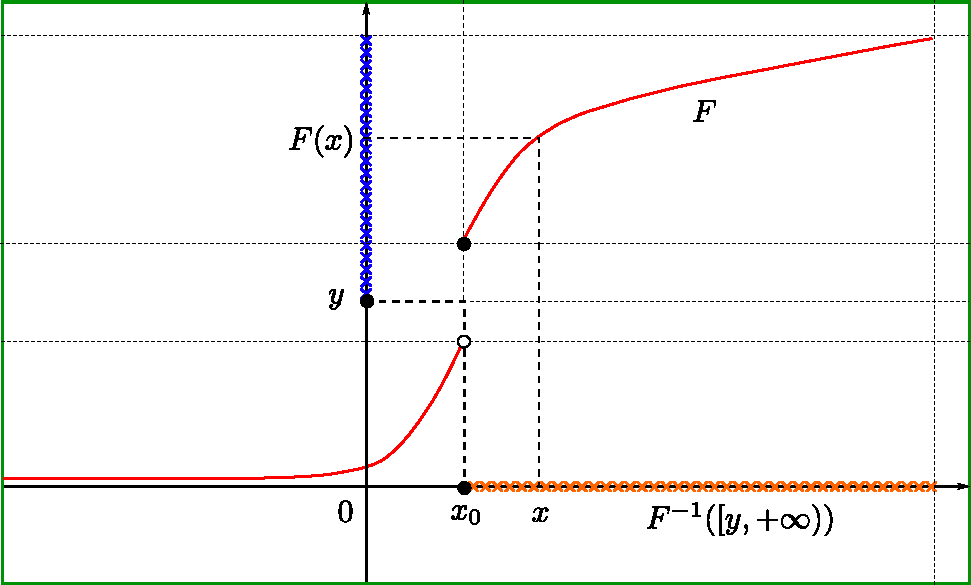
\includegraphics[width=0.8\textwidth]{Figuras/inversa-gen.pdf}
\caption{Esboço do gráfico de uma função distribuição $F$ descontínua.}
\label{Rotulo}
\end{figure}
\end{center}
%%%
\end{observacao}

\begin{proposicao}\label{prop-propriedades-G}
	Para todo $y\in (0,1)$ o conjunto $A(y)$ definido acima 
	tem as seguintes propriedades:
	\begin{enumerate}
		\item 
		$A(y)$ é um conjunto fechado.
		
		\item
		$\inf A(y) \in A(y)$, ou seja, $y\leq F(G(y))$.
		
		\item 
		$t<G(y)$ se, e somente se, $F(t)<y$.
		
		\item 
		$G(y)\leq t$ se, e somente se, $y\leq F(t)$.
	\end{enumerate}
\end{proposicao}


\begin{proof}
	{\bf Prova do item 1.} 
	Seja $\{s_n\}$ uma sequência em $A(y)$ tal que $s_n\to s$. 
	Note que $\{s_n\}$ possui pelo menos uma subsequência 
	monótona, não-crescente ou não-decrescente $\{s_{n_{k}}\}$ 
	que converge para $s$. Vamos considerar primeiro o caso 
	em que existe uma subsequência $s_{n_k}\downarrow s$. 
	Já que $s_{n_k}\in A(y)$ então 
	é válida a seguinte desigualdade $y\leq F(s_{n_k})$.
	Tomando nesta desigualdade o limite, quando $k\to\infty$, 
	obtemos da continuidade a direita de $F$ que 
		\[ 
			y \leq 
			\lim_{k\to\infty} F(s_{n_k}) 
			= 
			F(s).
		\]
	O que mostra que $s\in A(y)$.
	Por outro lado, se $\{s_n\}$ não possui uma subsequência 
	$s_{n_k}\downarrow s$, então existe no máximo uma quantidade
	finita de pontos da sequência $\{s_n\}$ 
	que é maior ou igual a $s$.
	Assim podemos afirmar que existe pelo menos 
	uma subsequência $s_{n_k}\uparrow s$
	tal que $s_{n_k} < s$. Usando  
	a definição de $A(y)$ e a monotonicidade de $F$ 
	temos que 
		\[
			y\leq F(s_{n_k})\leq F(s).
		\]
	Logo $s\in A(y)$ e isto conclui a prova de que $A(y)$ é 
	um subconjunto fechado da reta.
	
	{\bf Prova do item 2.} Segue diretamente da definição $\inf A(y)$,
	que 	existe uma sequência $\{s_n\}\subset A(y)$ tal que $s_n\to \inf A(y)$.
	Uma vez que o item 1 garante que $A(y)$ é fechado, temos que 
		\[G(y)=\inf A(y) \in A(y).\]
	 Segue então da definição de $A(y)$ que $y\leq F(G(y))$.


	{\bf Prova do item 3.} Note que $t<G(y)$ é equivalente a
	$t<\inf A(y)$. Esta desigualdade é equivalente a 
	$t\in A(y)^c$, isto é, $t\in\{s\in\R: F(s)<y\}$. 
	Como a última afirmação é equivalente a $F(t)<y$ a
	prova deste item está completa.
	
	
	{\bf Prova do item 4.} Se $G(y)\leq t$ então 
	segue do item 3 que 	$y\leq F(t)$. A recíproca é 
	também uma aplicação direta do item 3.  
	Isto completa a prova da proposição.
\end{proof}

\bigskip

Para cada $A\subset \R$ definimos agora o seguinte conjunto:
	\begin{equation}\label{def-xi-F}
		\xi_F(A) \equiv \{ x\in (0,1]: G(x)\in A \} = G^{-1}(A)\cap (0,1].
	\end{equation}
No lema seguinte mostramos que se $A$ 
é um boreliano de $\R$ (notação $A\in\mathscr{B}(\R)$)  
então 
$\xi_F(A)$ é um boreliano de $(0,1]$ 
(notação $\xi_F(A) \in\mathscr{B}((0,1])$).

\begin{lema}
	Se $A\in\mathscr{B}(\R)$ então $\xi_F(A) \in\mathscr{B}((0,1])$, onde
	$\xi_F(A)$ é definido como em \eqref{def-xi-F}.
\end{lema}



\begin{proof}
Considere a seguinte coleção 
	\[
		\mathscr{C} 
		=
		\{ A\subset\R: \xi_F(A) \in \mathscr{B}((0,1])\}.
	\]
Afirmamos que $\mathscr{C}$ contém qualquer intervalo finito da forma
$(a,b]\subset \R$. De fato, segue dos itens 3 e 4 
da Proposição \ref{prop-propriedades-G} que 
para todo $x\in (0,1)$ satisfazendo 
$a<G(x)$ temos $F(a)<x$ e por outro lado, se $G(x)\leq b$ temos 
$x\leq F(b)$. Da definição de $\xi_{F}(A)$ e 
das duas observações anteriores temos que
%
%
\begin{align*}
	\xi_F((a,b]) 
	&= 
	\{ x\in (0,1]: G(x) \in (a,b] \}
	\\
	&=	
	\{ x\in (0,1]: a<G(x)\leq b  \}
	\\
	&=
	\{ x\in (0,1]:F(a) <x \leq F(b) \}
	\\
	&=
	(F(a),F(b)].
\end{align*}
Como o lado direito acima pertence a $\mathscr{B}((0,1])$
segue que todo intervalo finito $(a,b]\in \mathscr{C}$.
Em outras palavras, a coleção $\mathscr{C}$ 
contém o $\pi$-sistema $\mathcal{G}=\{ (a,b]: a,b\in\R\}$.


Vamos mostrar agora que $\mathscr{C}$ é um $\lambda$-sistema. 
Para provar que $\R\in \mathscr{C}$, basta 
notar que
$
	\xi_F(\R)
	= G^{-1}(\mathbb{R})\cap (0,1] 
	= (0,1)\cap (0,1]
	\in \mathscr{B}((0,1]). 
$
Suponha que $A\in\mathscr{C}$, então 
$\xi_F(A)=G^{-1}(A)\cap (0,1]\in \mathscr{B}((0,1])$.
Pela propriedades de imagem inversa temos que 
\[
	G^{-1}(A^c)= \Big(G^{-1}(A)\Big)^c
\]
e como $\xi_F(A)$ é um boreliano de $(0,1]$, segue da definição 
de topologia induzida que 
	\[
		\xi_F(A^c)
		=
		G^{-1}(A^c)\cap (0,1]
		= 
		\Big(G^{-1}(A)\Big)^c\cap (0,1]		
	\]
é um boreliano de $(0,1]$, mostrando que $A^c\in\mathscr{C}$.

Se $\{A_n\}$ é uma família de 
conjuntos mutuamente disjuntos em $\mathscr{C}$,
então 
	\begin{align*}
	\xi_F\left( \bigcup_{n=1}^{\infty} A_n\right)
	=&
	G^{-1}\left( \bigcup_{n=1}^{\infty} A_n\right)\cap (0,1]
	\\
	=&
	\bigcup_{n=1}^{\infty} G^{-1}\left(A_n \right)\cap (0,1]
	\end{align*}
pertence a $\mathscr{B}((0,1])$. Logo $\cup_{n\geq 1} A_n\in \mathscr{C}$
o que prova encerra a prova de que $\mathscr{C}$ é um $\lambda$-sistema.

Pelo Teorema $\pi-\lambda$ de Dynkin $\mathscr{C}$ contém a $\sigma$-álgebra
gerada por $\mathcal{G}$ que é $\mathscr{B}(\R)$. Este fato 
completa a prova do lema.
\end{proof}

Finalmente podemos apresentar a definição de $\P_F$.
Para cada $A\in \mathscr{B}(\R)$ definimos 
	\[
		\P_{F}(A) =\lambda(\xi_{F}(A)),
	\]
onde $\lambda$ é a medida de Lebesgue em $(0,1]$.
É simples verificar que $\P_F$ é de fato uma medida
de probabilidade sobre $\mathbb{R}$ 
e que a função distribuição que ela induz é dada por
%
\begin{align*}
	\P_F((-\infty,x]) 
	&=
	\lambda \Big(\xi_{F}((-\infty,x])\Big)
	\\
	&=
	\lambda\Big( \{ y\in (0,1]: G(y)\in (-\infty,x] \} \Big)
	\\
	&=
	\lambda\Big( \{ y\in (0,1]: G(y)\leq x \} \Big)
	\\
	&=
	\lambda\Big( \{ y\in (0,1]: y\leq F(x) \} \Big)
	\qquad
	(\text{item 4 Proposição \ref{prop-propriedades-G}})
	\\
	&=
	\lambda\Big( (0,F(x)] \Big)
	\\
	&=
	F(x).
\end{align*}
















% Aula 5
\chapter[Aula 5]{Funções Mensuráveis Reais e Complexas}
\chaptermark{}

\section{Funções Mensuráveis}

A partir de agora usamos a notação $\overline{\R}$ 
para denotar a reta estendida, isto é, o conjunto
$\overline{\R} = \R\cup\{-\infty,+\infty\}$. 
Observe que podemos estender naturalmente conceito 
de soma e produto  de números reais
para os seguintes pares de elementos 
de $\overline{\R}$:
\begin{enumerate}
	\item 
	para quaisquer $x,y\in \R$ a soma é a soma usual 
	e o mesmo para o produto. 
	
	\item para todo $x\in \overline{\R}$ temos 
	$0\cdot x=0$.
	
	\item Para todo $x\in \overline{\R}$ diferente de 
	$-\infty$ definimos $x+(+\infty)=+\infty$.

	\item Para todo $x\in \overline{\R}$ diferente de 
	$+\infty$ definimos $x+(-\infty)=-\infty$.
	
	\item 
	$\pm \infty \cdot \pm \infty = +\infty$ 
	e
	$\pm \infty \cdot \mp \infty = -\infty$.
	
\end{enumerate}

Não vamos nos preocupar, neste momento, em munir $\overline{\R}$ 
de uma topologia, mas vamos definir a $\sigma$-álgebra
de Borel de $\overline{\R}$,
como sendo a coleção formada pela reunião da
coleção $\mathscr{B}(\R)$ 
e de todos conjuntos da forma 
$B\cup\{-\infty\}$, $B\cup\{+\infty\}$ e $B\cup\{-\infty,+\infty\}$,
onde $B$ varia sobre todos os elementos de $\mathscr{B}(\R)$.
Esta coleção que acabamos de definir
é de fato uma $\sigma$-álgebra e será chamada de $\sigma$-álgebra
de borel de $\overline{\R}$ e denotada por $\mathscr{B}(\overline{\R})$.

\begin{exercicio}
	Mostre que a coleção $\mathscr{B}(\overline{\R})$ 
	é uma $\sigma$-álgebra.
\end{exercicio}

\begin{exercicio}
	Podemos ver $\overline{\R}$ como um conjunto totalmente ordenado se 
	consideramos a relação de ordem ``$<$'' obtida pela extensão natural 
	da relação de ordem em $\R$.
	Seja $\tau$ a topologia da ordem definida por ``$<$'' 
	em $\overline{\R}$. Mostre que a $\sigma$-álgebra gerada pelos 
	abertos de $\tau$ coincide com a coleção $\mathscr{B}(\overline{\R})$
	definida acima. 
	
\end{exercicio}










\subsection*{Funções a Valores Reais Mensuráveis}

Nesta subseção vamos considerar funções que
saem de um espaço mensurável $(\Omega,\F)$ e tomam 
valores em $\mathbb{R}$. O caso mais geral, onde
as funções assumem valores em $\overline{\mathbb{R}}$ será
tratado na subseção seguinte.


\begin{definicao} 
Seja $(\Omega,\F)$ um espaço mensurável. 
Uma função $f:\Omega\to\R$ é dita $\F$-mensurável
se para todo número real $\alpha$ temos que
\[
	\{\omega \in\Omega : f(\omega)>\alpha \} \in \F.
\]
\end{definicao}

O próximo lema fornece três maneira alternativas de
definir funções mensuráveis. 

\begin{lema}\label{lema-equiv-mensuravel-borel}
As seguintes afirmações são equivalentes para uma função 
$f:\Omega\to\R$.
\begin{enumerate}
	\item 
	Para todo $\alpha\in\R$ o conjunto 
	$A_{\alpha}\equiv\{\omega\in\Omega : f(\omega)>\alpha \} \in \F$.

	\item 
	Para todo $\alpha\in\R$ o conjunto 
	$B_{\alpha}\equiv\{\omega\in\Omega : f(\omega)\leq \alpha \} \in \F$.

	\item 
	Para todo $\alpha\in\R$ o conjunto 
	$C_{\alpha}\equiv\{\omega\in\Omega : f(\omega)\geq\alpha \} \in \F$.

	\item 
	Para todo $\alpha\in\R$ o conjunto 
	$D_{\alpha}\equiv\{\omega\in\Omega : f(\omega)<\alpha \} \in \F$.
	
\end{enumerate}
\end{lema}


\begin{proof}
	Já que $A_{\alpha}$ e $B_{\alpha}$ são complementares um do outro
	temos imediatamente que 1 e 2 são equivalentes. Pelo mesmo 
	motivo segue que 3 e 4 são equivalentes. Vamos assumir agora que 
	1 seja válido. Então temos que $A_{\alpha-1/n}\in \F$ para todo
	$n\in\N$. Já que 
	\[ 
		C_{\alpha} = \bigcap_{n=1}^{\infty} A_{\alpha-1/n} 
	\]
	temos que 1 implica 3. Por outro lado, a igualdade
	\[
		A_{\alpha} = \bigcup_{n=1}^{\infty} C_{\alpha+1/n}
	\]
	mostra que 3 implica 1.
\end{proof}






\begin{exercicio}
Seja $f:\Omega\to\mathbb{R}$ uma função definida
em um espaço mensurável $(\Omega,\F)$.
Mostre que $f$ é uma função $\F$-mensurável
se, e somente se, a coleção 
\[
f^{-1}(\mathscr{B}(\mathbb{R}))
\equiv
\{
f^{-1}(B):\ B\ \mathrm{\acute{e} \ um\ boreliano\ de}\ \mathbb{R}
\}.
\]
é uma sub-$\sigma$-álgebra de $\F$.
\end{exercicio}














\begin{exemplo}\label{exemplo-func-const.mensuravel}
	Toda função constante $f:\Omega\to\R$ é mensurável.
	De fato, se $f(\omega)=c$ para todo $\omega\in\Omega$ 
	então temos que se $\alpha\geq c$ então 
	$\{\omega\in\Omega: f(\omega)>\alpha\} =\emptyset$.
	Por outro lado, se $\alpha<c$ então 
	$\{\omega\in\Omega: f(\omega)>\alpha\} =\Omega$.
\end{exemplo}





\begin{exemplo}
	Seja $(\Omega,\F)$ um espaço mensurável. 
	Se $E\in\F$ então a função $1_E:\Omega\to\R$, a função indicadora de $E$,
	é mensurável e vice-versa.
	Para ver que a afirmação é verdadeira basta notar que 
	$\{\omega\in\Omega: 1_{E}(\omega)>\alpha \}$ é igual $\Omega, E$
	ou $\emptyset$.
\end{exemplo}



\begin{exemplo}
	Considere o espaço mensurável $(\R,\mathscr{B}(\R))$. 
	Então qualquer função $f:\R\to\R$ contínua é 
	$\mathscr{B}(\R)$-mensurável.
	Basta notar que para todo $\alpha\in \R$ temos
	por continuidade que $\{x\in\R: f(x)>\alpha\}$ é 
	um aberto da reta e portanto pertence a $\sigma$-álgebra
	de borel de $\R$.
\end{exemplo}




\begin{exemplo}
	Considere o espaço mensurável $(\R,\mathscr{B}(\R))$ e 
	seja $f:\R\to\R$ uma função monótona não-decrescente.
	Para qualquer $\alpha\in\R$, 
	temos que $\{x\in\R: f(x)<\alpha\}$ ou é uma semi-reta
	da forma $(-\infty,a)$ ou $(-\infty,a]$ ou $\R$ ou $\emptyset$.
	Portanto toda função monótona não-decrescente é borel 
	mensurável, isto é, $\mathscr{B}(\R)$-mensurável.
\end{exemplo}


Vamos mostrar na sequência que algumas operações algébricas
entre funções mensuráveis fornece também uma função mensurável.

\begin{lema}\label{lema-operacoes-alg-com-func-mensuraveis}
	Sejam $(\Omega,\F)$ um espaço de medida e 
	$f,g:\Omega\to\R$ funções $\F$-mensuráveis 
	e $c$ uma constante real. Então as funções 
	\[
		cf,\ f^2,\ f+g,\ fg,\ |f|
	\]
 	são também funções $\F$-mensuráveis.
\end{lema} 


\begin{proof}
Vamos mostrar primeiro que $cf$ é mensurável. 
Se $c=0$ então $cf\equiv 0$ e a mensurabilidade de $cf$
segue do Exemplo \ref{exemplo-func-const.mensuravel}.
Se $c>0$, para todo $\alpha\in\R$ temos que
\[ 
	\{ \omega\in \Omega: cf(\omega)>\alpha\}
	=
	\left\{ \omega\in \Omega: f(\omega)>\frac{\alpha}{c} \right\}
	\in \F.
\]
O caso $\alpha<0$ é análogo.

Vamos provar agora que $f^2$ é $\F$-mensurável. 
Vamos dividir o argumento em 
dois casos, $\alpha<0$ e $\alpha \geq 0$.
No primeiro caso $\alpha<0$, temos que 
$\{ \omega\in \Omega: f^2(\omega)>\alpha\} = \Omega$
Se $\alpha\geq 0$ então 
\[ 
	\{ \omega\in \Omega: f^2(\omega)>\alpha\} 
	=
	\{ \omega\in \Omega: f(\omega)>\sqrt{\alpha}\} 
	\cup
	\{ \omega\in \Omega: f(\omega)<-\sqrt{\alpha}\}
	\in 
	\F. 
\]

Passamos agora para a mensurabilidade da soma. 
Por hipótese para qualquer número racional $r$
e qualquer que seja $\alpha\in\R$, temos que 
\[
	S_r
	\equiv 
	\{ \omega\in\Omega: f(\omega)>r \} 
		\cap 
		\{ \omega\in\Omega: g(\omega)>\alpha-r \}
	\in 
	\F.
\]
Já que 
\[
	\{ \omega\in\Omega: (f+g)(\omega)>\alpha \}
	=
	\bigcup_{r\in \Q} S_r
\]
é um conjunto $\F$-mensurável, segue que $f+g$ é mensurável.

Para mostrar que o produto $fg$ é mensurável, basta 
notar que 
\[ fg = \frac{1}{4}[(f+g)^2-(f-g)^2] \]
e usar o resultados provados acima.

Resta mostrar que $|f|$ é mensurável.
Novamente consideramos dois casos, $\alpha<0$ e 
$\alpha\geq 0$. No primeiro caso, $\alpha<0$, temos que 
$\{\omega\in\Omega: |f(\omega)|>\alpha\} = \Omega$.
Por outro lado, se $\alpha\geq 0$ então 
\[ 
	\{\omega\in\Omega: |f(\omega)|>\alpha\} 
	= 
	\{\omega\in\Omega: f(\omega)>\alpha\} 
	\cup
	\{\omega\in\Omega: f(\omega)<-\alpha\} .
\]
como ambos conjuntos do lado direito da igualdade 
acima pertencem a $\F$, segue que 
$\{\omega\in\Omega: |f(\omega)|>\alpha\} \in \F$ o que 
encerra a prova do lema.
\end{proof}


\subsection*{Partes Positiva e Negativa de Funções a Valores Reais}

A cada função $f:\Omega\to\mathbb{R}$ podemos associar duas funções 
{\bf não-negativas} denotadas por $f^+$ e $f^-$ ambas definidas em $\Omega$
por 
	\[
		f^+(\omega)= \sup\{f(\omega),0\} 
		\qquad
		\text{e}
		\qquad
		f^-(\omega)= \sup\{-f(\omega),0\} 
	\]
As funções $f^+$ e $f^-$ são chamadas, respectivamente 
de {\bf parte positiva} e {\bf parte negativa} de $f$.

Note que para qualquer que seja $\omega\in\Omega$, sempre temos
	\[
		f(\omega) = f^+(\omega)-f^{-}(\omega)
		\qquad
		\text{e}
		\qquad
		|f(\omega)| = f^+(\omega)+f^{-}(\omega).
	\]
	
	
\begin{lema}
	Seja $(\Omega,\F)$ um espaço de medida. Uma função 
	$f:\Omega\to\R$, é $\F$-mensurável se, e somente se,
	$f^+$ e $f^-$ são $\F$-mensuráveis.
\end{lema}

\begin{proof}
A prova deste lema é consequência direta das seguintes identidades:
\[
	f^{+} = \frac{1}{2}(|f|+f)
	\qquad
	\text{e}
	\qquad
	f^{-} = \frac{1}{2}(|f|-f).
\]
\end{proof}


Até o momento trabalhamos com o conceito de mensurabilidade em 
$\R$. Como frequentemente iremos trabalhar com sequências de 
funções e estaremos interessados em tomar, supremos, ínfimos,
limites e etc... é tecnicamente conveniente trabalhar com o 
conjunto $\overline{\R}$. Esta é a razão de introduzirmos 
na seção seguinte o conceito de mensurabilidade de uma função 
tomando valores na reta estendida. 






\section{Funções a Valores em $\overline{\R}$ Mensuráveis}

\begin{definicao}[Função Mensurável em $\overline{\R}$]
Seja $(\Omega,\F)$ um espaço de mensurável. Uma função 
$f:\Omega\to\overline{\R}$ é dita $\F$-mensurável, se para todo
$\alpha\in\R$ temos que 
$\{\omega\in\Omega:f(\omega)>\alpha\}\in\F$.
\end{definicao}


A coleção de todas as funções $\F$-mensuráveis 
tomando valores em $\overline{\R}$ é denotada por
$M(\Omega,\F)$. Observe que se $f\in M(\Omega,\F)$
então 
%
\[
\begin{array}{c}
	\displaystyle
	\{ \omega\in\Omega: f(\omega)=+\infty \}
	=
	\bigcap_{n=1}^{\infty} \{x\in\Omega: f(x)>n\}
	\\[0.3cm]
	\text{e}
	\\[0.3cm]
	\displaystyle
	\{ \omega\in\Omega: f(\omega)=-\infty \}
	=
	\left( 
		\bigcup_{n=1}^{\infty} \{x\in\Omega: f(x)>-n\}
	\right)^c
\end{array}
\]
são conjuntos $\F$-mensuráveis.



O próximo lema apresenta uma caracterização 
do conceito de mensurabilidade que acabamos de introduzir.
Ele será muito útil para provar mensurabilidade de funções
tomando valores em $\overline{\R}$. 


\begin{lema}\label{lema-truncamento-func-mensuravel-eh-mensuravel}
	Seja $(\Omega,\F)$ um espaço de medida. 
	Uma função $f:\Omega\to\overline{\mathbb{R}}$ é 
	mensurável se, e somente se, os conjuntos 
	\[
	A=\{ \omega\in\Omega: f(\omega)=+\infty \}
	\quad
	\mathrm{e}
	\quad
	B=\{ \omega\in\Omega: f(\omega)=-\infty \}	
	\]
	são $\F$-mensuráveis e a função  
	$f_{1}:\Omega\to\R$ dada por 
	\[
	f_1(\omega)=
		\begin{cases}
			f(x),&\text{se}\ x\notin A\cup B;
			\\
			0,&\text{se}\ x\in A\cup B.
		\end{cases}
	\]
	é $\F$-mensurável.
\end{lema}



\begin{proof}
Suponha que a função $f$ seja $\F$ mensurável. 
Como já observamos, se $f\in M(\Omega,\F)$ então $A$ e $B$ 
são $\F$-mensuráveis. Seja $\alpha\in \R$. Se $\alpha\geq 0$
então temos que 
\[
	\{\omega\in\Omega:f_1(\omega)>\alpha\}
	=
	\{\omega\in\Omega:f(\omega)>\alpha\}
	\setminus A.	
\] 
Se $\alpha<0$ então 
\[	
	\{\omega\in\Omega:f_1(\omega)>\alpha\}
	=
	\{\omega\in\Omega:f(\omega)>\alpha\}
	\cup B.	
\]
Portanto podemos concluir que $f_1$ é $\F$-mensurável.


Reciprocamente, suponha que $f_1\in M(\Omega,\F)$ e $A,B\in\F$.
Então para $\alpha\geq 0$ temos
\[
	\{\omega\in\Omega:f(\omega)>\alpha\}
	=
	\{\omega\in\Omega:f_1(\omega)>\alpha\}
	\cup A	
\] 
e se $\alpha<0$ temos que
\[
	\{\omega\in\Omega:f(\omega)>\alpha\}
	=
	\{\omega\in\Omega:f_1(\omega)>\alpha\}
	\setminus B,	
\] 
o que mostra que $f\in M(\Omega,\F)$.
\end{proof}



\begin{corolario}
	Seja $(\Omega,\F)$ um espaço de medida. Se $f\in M(\Omega,\F)$
	então para toda constante $c\in \R$ temos que 
	as funções $cf,\ f^2,\ |f|,\ f^{+}$ e $f^{-}\in M(\Omega,\F)$. 
\end{corolario} 

\begin{proof}
A prova é uma aplicação dos Lemas 
\ref{lema-operacoes-alg-com-func-mensuraveis} 
e
\ref{lema-truncamento-func-mensuravel-eh-mensuravel}.
Para exemplificar vamos mostrar que $f^2\in M(\Omega,\F)$. 
Vamos mostrar primeiro que $(f^2)_1=f_1f_1$.
Sejam $A$ e $B$ os conjuntos definidos no Lema 
\ref{lema-truncamento-func-mensuravel-eh-mensuravel}
com respeito a função $f$.
Se $\omega \notin A\cup B$, então 
$f(\omega)\in\R$ e assim $(f^2)_1(\omega)=f^2(\omega) = f_1(\omega)f_1(\omega)$.
Por outro lado, se $\omega\in A\cup B$ então temos que 
$(f^2)_1(\omega)= 0\cdot 0 = f_1(\omega)f_1(\omega)$.
Já que $(f^2)_1=f_1f_1$ segue do 
Lema \ref{lema-operacoes-alg-com-func-mensuraveis} 
que $(f^2)_1$ é mensurável. Observando que os conjuntos 
$A$ e $B$ para $f^2$ são $\F$-mensuráveis segue do 
Lema \ref{lema-truncamento-func-mensuravel-eh-mensuravel}
que $f^2$ é $\F$-mensurável.
\end{proof}



\begin{observacao}
Se $f$ e $g$ pertencem a $M(\Omega,\F)$, então a função 
soma $(f+g)(\omega)$ não está bem definida pela fórmula 
$(f+g)(\omega)=f(\omega)+g(\omega)$ nos seguintes conjuntos:
\[
\begin{array}{c}
	E_1=\{\omega\in\Omega: f(\omega)=+\infty\ \text{e}\ g(\omega)=-\infty\}
	\\
	\text{e}
	\\
	E_2=\{\omega\in\Omega: f(\omega)=-\infty\ \text{e}\ g(\omega)=+\infty\}.
\end{array}
\] 
Note que $E_1$ e $E_2\in \F$. Assim se definimos $(f+g)$ 
sobre a união destes conjuntos como sendo zero, 
então a função resultante é $\F$-mensurável. 
Após o lema seguinte vamos discutir sobre a mensurabilidade
de $fg$.
\end{observacao}



\begin{lema}\label{inf-sup-func-mensuraval-eh-mensuravel}
	Seja $\{f_n\}$ uma sequência de funções em $M(\Omega,\F)$.
	Defina as seguintes funções:
	\[	
	\begin{array}{cc}
	\displaystyle
	f(\omega) = \inf_{n\to\infty}f_n(\omega), & 	
	\displaystyle
	F(\omega) = \sup_{n\to\infty}f_n(\omega),
	%
	\\[0.5cm]
	\displaystyle
	f^*(\omega) = \liminf_{n\to\infty}f_n(\omega), & 	
	\displaystyle
	F^*(\omega) = \limsup_{n\to\infty}f_n(\omega).	
	\end{array}
	\]
Então $f,F,f^*$ e $F^*$ pertencem a $M(\Omega,\F)$.
\end{lema}


\begin{proof}
Para cada $n\in\N$ fixado, segue da 
hipótese de mensurabilidade de $f_n$ que 
o seguinte conjunto é $\F$-mensurável
\[
\{\omega\in\Omega: f_n(\omega)\geq \alpha\}
=
\bigcap_{k=1}^{\infty}
\left\{
	\omega\in\Omega: f_n(\omega)>\alpha-\frac{1}{k} 
\right\}. 
\]
Como as seguinte igualdade são válidas:
	\[	
	\{\omega\in\Omega: f(\omega)\geq \alpha\} 
	=
	\bigcap_{n=1}^{\infty}
	\left\{
		\omega\in\Omega: f_n(\omega)\geq \alpha 
	\right\}
	\]
e
 	\[
 	\{\omega\in\Omega: F(\omega)> \alpha\} 
	=
	\bigcup_{n=1}^{\infty}
	\left\{
		\omega\in\Omega: f_n(\omega)> \alpha 
	\right\}
	\]
temos que $f$ e $F$ são mensuráveis sempre que $f_n$
é mensurável para todo $n\in\N$.
Já que 
	\[	
	f^*(\omega)
	=
	\sup_{n\geq 1}
	\left\{ \inf_{m\geq n} f_{m}(\omega) \right\}
	\quad
	\text{e}
	\quad
	F^*(\omega)
	=
	\inf_{n\geq 1}
	\left\{ \sup_{m\geq n} f_{m}(\omega) \right\}
	\]
basta aplicar duas vezes consecutivas o resultado que acabamos 
de provar para concluir que ambas $f^*$ e $F^*$ são $\F$-mensuráveis.
\end{proof}




\begin{corolario}\label{cor-lim-mensuravel-eh-mensuravel}
Se $\{f_n\}$ é uma sequência em $M(\Omega,\F)$ tal que
$f_n(\omega)\to f(\omega)$ para todo $\omega\in\Omega$,
então $f\in M(\Omega,\F)$.
\end{corolario} 

\begin{proof}
	Basta observar que 
		\[
			f(\omega) 
			=\limsup_{n\to\infty} f_n(\omega)
			=\liminf_{n\to\infty} f_n(\omega).
		\]
\end{proof}


Voltamos a questão da mensurabilidade do produto $fg$,
quando ambas $f$ e $g\in M(\Omega,\F)$. Para isto 
vamos introduzir a noção de truncamento de uma função em 
$M(\Omega,\F)$. Para cada $n\in\N$ considere a função 
$f_n$ que é chamada de um truncamento de $f$, definida por 
	\[
		f_n(\omega)
		=
		\begin{cases}
			f(\omega),&\text{se}\ |f(\omega)|\leq n;
			\\
			n,&\text{se}\ f(\omega)>n;
			\\
			-n,&\text{se}\ f(\omega)<-n.
		\end{cases}
	\]
\begin{exercicio}
	Sejam $f\in M(\Omega,\F)$ e $n\in\N$. 
	Mostre que se $f_n$ é um truncamento de $f$, 
	como definido acima, então $f_n\in M(\Omega,\F)$. 
\end{exercicio}

Se $f_n$ e $g_m$ são truncamentos de $f$ e $g$, respectivamente
segue do Lema \ref{lema-operacoes-alg-com-func-mensuraveis}
que o produto $f_n\cdot g_m$ é mensurável. Já que 
para todo $\omega\in \Omega$ temos 
	\[
		f(\omega)g_m(\omega) 
		=
		\lim_{n\to\infty} f_n(\omega)g_m(\omega)
	\]
segue do Corolário \ref{cor-lim-mensuravel-eh-mensuravel}
que $fg_m \in M(\Omega,\F)$. Observando que
	\[
		(fg)(\omega) 
		=
		f(\omega)g(\omega)
		=
		\lim_{m\to\infty} f(\omega)g_m(\omega)
	\]	
outra aplicação do Corolário \ref{cor-lim-mensuravel-eh-mensuravel}
mostra finalmente que $fg\in M(\Omega,\F)$.




\begin{definicao}[Sequência Monótona de Funções]
 Uma sequência $\{f_n\}$ em $M(\Omega,\F)$ é dita
 monótona não-decrescente, se para todo $\omega\in\Omega$
 fixado, temos que 
 	\[
 		f_n(\omega)\leq f_{n+1}(\omega)
 		\quad
 		\forall n\in\N.
 	\]
Analogamente definimos sequências monótonas não-crescentes.
\end{definicao}




\begin{definicao}[Função Simples]
Seja $(\Omega,\F)$ um espaço mensurável. 
Uma função $f:\Omega\to\overline{\mathbb{R}}$ é dita 
simples se assume no máximo uma quantidade
finita de valores, isto é, $\# f(\Omega)<\infty$.

\end{definicao}



O Corolário \ref{cor-lim-mensuravel-eh-mensuravel} afirma que 
limite pontual de funções em $M(\Omega,\F)$ é uma função em 
$M(\Omega,\F)$.
Assumindo apenas que $f$ é não-negativa e mensurável
mostramos no próximo lema um fato ainda mais
forte. Sob estas condições vamos ver que  
$f$ é limite pontual de alguma sequência 
monótona não-decrescente de funções 
simples $f_n$ em $M(\Omega,\F)$,
além do mais a demostração fornece uma maneira de construir
tal sequência.

\begin{teorema}\label{teo:aproximacao-monotona-por-func-simples}
	Seja $(\Omega,\F)$ um espaço de medida. 
	Se $f:\Omega\to [0,+\infty]$
	é uma função mensurável, 
	existe uma sequência de funções 
	simples $f_n:\Omega\to[0,\infty]$ tal que
	para todo $\omega\in\Omega$ temos
	$0\leq f_1(\omega)\leq f_2(\omega)\leq \ldots\leq f(\omega)$ 
	e 
	$f_n(\omega)\to f(\omega)$.
\end{teorema}


\begin{proof} 
Fixe $n\in\mathbb{N}$ e considere uma partição do 
intervalo $[0,n)$ em intervalos semi-abertos de
mesmo comprimento igual a $1/2^n$, da seguinte 
forma:
\[
[0,n)
=
\left[ 0,\frac{1}{2^n} \right) 
\cup
\left[ \frac{1}{2^n},\frac{2}{2^n} \right) 
\cup
\ldots
\cup 
\left[ \frac{k}{2^n},\frac{k+1}{2^n} \right) 
\cup
\ldots
\cup
\left[ \frac{n2^n-1}{2^n}, \frac{n2^n}{2^n} \right).
\]
Estes $n2^n$ intervalos 
junto com o intervalo $[n,+\infty]$ formam uma partição 
de $[0,+\infty]$. 
%
Esta partição induz uma partição em $\Omega$
que é determinada pelas pré-imagens destes conjuntos 
por $f$, isto é, para $k\in\mathbb{N}$ satisfazendo 
$0\leq k\leq n2^{n}-1$, defina
\[
E_{n}^{k}=
f^{-1}\left( \left[\frac{k}{2^n},\frac{k+1}{2^n} \right) \right)
\qquad \text{e} \qquad
E_n^{n2^n}=f^{-1}\big( [n,+\infty]\big).
\]
Com auxilio desta partição, 
definimos uma sequência de funções simples
não-negativas $\{f_n\}$, onde 
\[
f_n =\sum_{k=0}^{n2^n-1} \frac{k}{2^n} 1_{E_{n}^{k}} + n 1_{E_n^{n2^n}}.
\]

Segue diretamente da definição dos conjuntos 
$E_{n}^{k}$ que $f_n(\omega)\leq f_{n+1}(\omega)$ 
para todo $\omega\in\Omega$.
Note também que se $f(\omega)<n$ 
então $0\leq f(\omega)-f_n(\omega)<\frac{1}{2^n}$. 
Por outro lado, se 
$f(\omega)=+\infty$ temos que $f_n(\omega)= n$,
logo $f_n(\omega)\to+\infty$.
Portanto para todo $\omega\in\Omega$ temos que 
$f_n(\omega)\to f(\omega)$, quando $n\to\infty$.
\end{proof}

\begin{observacao} 
O leitor mais atento deve ter notado que 
a última estimativa apresentada na demonstração acima 
implica que a convergência das funções simples $f_n$ 
para $f$ é uniforme nos conjuntos 
onde $f$ é limitada, isto é, dado $M>0$ 
seja $\Omega_M=\{\omega\in\Omega; f(\omega)\leq M\}$ então a sequência 
$f_n|_{\Omega_M}\to f|_{\Omega_M}$ uniformemente.
\end{observacao}

 







\section{Funções Mensuráveis a Valores Complexos}

É de grande importância na Teoria da Probabilidade 
o estudo de algumas funções a valores complexos
como, por exemplo, as chamadas funções 
características. 
Por isto, vamos introduzir nesta pequena seção a noção
de mensurabilidade para tais funções. Observe que 
se $f$ é uma função complexa definida em $\Omega$,
isto é, $f:\Omega\to\C$ é uma função, então existem
duas outras funções reais unicamente determinadas
chamadas respectivamente, de partes real e imaginária
denotadas por $u,v:\Omega\to\R$ tais que 
	\[
	f(\omega) =u(\omega)+iv(\omega),
	\]
onde $u(\omega)=\text{Re}(f(\omega))$ e
$v(\omega)=\text{Im}(f(\omega))$.
\begin{definicao}
[Função Complexa Mensurável]
Seja $(\Omega,\F)$ um espaço de medida. 
Uma função complexa $f:\Omega\to\C$ é dita 
mensurável se, e somente se, suas partes 
real e imaginária são funções mensuráveis.
\end{definicao} 

\begin{exercicio}
Mostre que somas, produtos e limites de funções complexas 
mensuráveis é uma função complexa mensurável.
\end{exercicio}










% Lista 1
\chapter*{Lista 1}
\addcontentsline{toc}{chapter}{Lista 1}
\chaptermark{}
%%%%%%%%%%%%%%%%%%%%%%%%%%%%%%%%%%%%%%%%%%%%%%%%

% Inicio da Lista de Exercícios 
\begin{enumerate}[leftmargin=*]


\item 
Seja $\Omega$ um espaço não vazio. 
Seja $\F_0$ a coleção de todos os 
subconjuntos $E\subset\Omega$ 
tais que $E$ ou $E^c$ é vazio.
Considere a função de conjuntos $P:\F_0\to [0,1]$
definida por 
	\[
		P(E) =
		\begin{cases}
		0,&\text{se}\ E \ \text{é finito};
		\\
		1,&\text{se}\ E^c \ \text{é finito}.
		\end{cases}
	\]
	\begin{itemize}
		\item[a)]
		Mostre que $\F_0$ é uma álgebra de conjuntos.
		
		\item[b)] 
		Assumindo que $\Omega$ é um conjunto infinito enumerável,
		mostre que $P$ é finitamente aditiva, mas não é $\sigma$-aditiva.
		
		\item[c)]
		Assumindo que $\Omega$ é não-enumerável, mostre que $P$ 
		é $\sigma$-aditiva em $\F_0$.
		
	\end{itemize}





\item 
Seja $(\Omega,\F,\P)$ um espaço de probabilidade.
Se para todo $n\in\N$ o evento 
$B_n\subset A_n$ então mostre que 
	\[
		\P\left( \bigcup_{n=1}^{\infty} A_n \right)
		-\P\left( \bigcup_{n=1}^{\infty} B_n  \right)	
		\leq 
		\sum_{n=1}^{\infty} \Big( \P(A_n)-\P(B_n) \Big)	
	\]





\item 
Seja $(\Omega,\F)$ um espaço de mensurável. 
Suponha que $\P$ é uma medida de probabilidade
definida em $\F$ e que existe um conjunto $A\subset\Omega$
tal que $A\notin\F$. Considere a $\sigma$-álgebra 
$\F_1 = \sigma(\F,A)$. Mostre que $\P$ admite uma extensão 
a uma medida de probabilidade $\P_1$ definida em $\F_1$. 





\item 
Seja $\P$ uma medida de probabilidade em $\mathscr{B}(\R)$.
Mostre que para qualquer $B\in \mathscr{B}(\R)$ e $\varepsilon>0$ 
dado, existe uma união finita de intervalos $A$ tal que 
	\[
		\P(A\bigtriangleup B) < \varepsilon.
	\]
\noindent{ Dica.} Defina a seguinte coleção:
\[ 
	\mathscr{C}
	=
	\{
		B\in\mathscr{B}(\R): \forall \varepsilon>0,
		\exists A_{\varepsilon} (\text{união finita de interv.})
		\ \text{tal que} \P(A_{\varepsilon} \bigtriangleup B)<\varepsilon
	\}
\]



\item 
Dizemos uma sequência de eventos $\{A_n\}$ 
em um espaço de probabilidade
$(\Omega,\F,\P)$ é quase disjunta se 
$\P(A_i\cap A_j)=0$ se $i\neq j$. 
Para tais eventos mostre que 
\[
	\P\left( \bigcup_{n=1}^{\infty} A_n \right)
	=
	\sum_{n=1}^{\infty} \P(A_n).
\]







\item Sabemos que $\P_1=\P_2$ em $\F$ dado que $\P_1=\P_2$
em $\mathcal{C}$ e $\mathcal{C}$ é $\pi$-sistema 
que gera $\F$. 
Mostre que a hipótese de $\mathcal{C}$ ser um $\pi$-sistema
não pode ser removida, através do seguinte exemplo:
considere $\Omega=\{a,b,c,d\}$ e que 
\[
	\P_1(\{a\}) = \P_1(\{d\}) = \P_2(\{b\}) = \P_2(\{c\}) = \frac{1}{6}
\]
e
\[
	\P_1(\{b\}) = \P_1(\{c\}) = \P_2(\{a\}) = \P_2(\{d\}) = \frac{1}{3}.
\]
Tome $\mathcal{C}=\{ \{a,b\}, \{d,c\}, \{a,c\}, \{b,d\} \}$.












\item 
{\bf Definição.} \index{Conjuntos!$\P$ equivalentes}
Seja $(\Omega,\F,\P)$ um espaço de probabilidade. 
Dizemos que dois conjuntos $A,B\in \F$ são equivalentes
se $\P(A\bigtriangleup B)=0$. A classe de equivalência
do envento $A$ é dada por 
\[ 
	[A] = \{B\in \F: \P(A \bigtriangleup B)=0 \}.
\]
Desta forma podemos decompor $\F$ em classes de equivalência.
\\
{\bf Definição.} Um átomo \index{Átomo} em um espaço 
de probabilidade $(\Omega,\F,\P)$ é definido como sendo
um conjunto $A\in\F$ tal que $P(A)>0$ e se 
$B\subset A$ e $B\in \F$, então $\P(B)=0$ ou 
$P(A\setminus B)=0$. 
Além do mais o espaço de probabilidade é dito não-atômico
se ele não possui átomos, isto é, se $A\in F$ e 
$P(A)>0$ então existe pelo menos um evento $B\in \F$ tal que
$B\subset A$ e $0<P(B)<P(A)$.

	\begin{itemize}
		\item[a)]
		Se $\Omega=\R$ e $\P$ é determinada por uma 
		função distribuição $F$, mostre que os átomos
		são $\{x\in\R: F(x)-F(x-)>0\}$.
				
		\item[b)]
		Mostre que o espaço de probabilidade  
		$(\Omega,\F,\P)=((0,1],\mathscr{B}((0,1]),\lambda)$,
		onde $\lambda$ é a medida de Lebesgue, é não-atômico. 

		\item[c)]
		Mostre que se $A$ e $B$ são átomos tais que
		$\P(A\bigtriangleup B)>0$ então temos que
		$\P((A\cap B) \bigtriangleup \emptyset)=0$.


		\item[d)] 
		Um espaço de probabilidade contém no máximo 
		uma quantidade enumerável de átomos. 
		\\
		(Dica. Qual é o número máximo de átomos que o
		espaço pode conter tendo probabilidade pelo menos $1/n$\ ?)
		
		
		\item[e)]
		Se um espaço de probabilidade $(\Omega,\F,\P)$
		não contém átomos, então para todo $a\in (0,1]$
		existe pelo menos um conjunto $A\in\F$ tal que 
		$\P(A)=a$. 
		\\
		(Uma maneira de provar este fato é usando o Lema de Zorn.)
	\end{itemize}






\item
Suponha que $\{E_n\}$ é uma sequência de eventos tal que
para todo $n\in\mathbb{N}$ temos $\P(E_n)=1$. Mostre que 
\[	
	\P\left(  \bigcap_{n=1}^{\infty} E_n\right) =1 
\]






\item
Suponha que $\mathcal{C}$ seja uma coleção de subconjuntos de 
$\Omega$ e que $B\subset \Omega$ é um evento satisfazendo
$B\in\sigma(\mathcal{C})$.
Mostre que existe uma coleção enumerável $\mathcal{C}_{B}$
tal que $B\in \sigma(\mathcal{C}_{B})$.
\\
(Dica. Considere o conjunto 
$\mathcal{G}=\{ B\subset\Omega: \exists\ \text{uma coleção enumerável}\ 
\mathcal{C}_B\subset \mathcal{C}\ 
\text{tal que}\ B\in\sigma(\mathcal{C}_{B}) \}
$
e mostre que $\mathcal{G}$ é uma $\sigma$-álgebra contendo
$\mathcal{C}$.)







\item 
Se $\{E_k\}$ é uma coleção de eventos tal que 
	\[
		\sum_{k=1}^{n} \P(E_k) > n-1
	\]
então 
\[	
	\P\left(  \bigcap_{n=1}^{n} E_n\right) >0. 
\]	






\item 
Mostre que se $F$ é uma função distribuição, 
então $F$ tem no máximo uma quantidade enumerável 
de descontinuidades.






\item 
Seja $F$ uma função distribuição e considere as seguintes
funções $G,H:(0,1)\to \mathbb{R}$ dadas por 
	\[
		G(y)= \inf\{t\in\mathbb{R}: y\leq F(t) \}
		\quad
		\text{e}
		\quad
		H(y)= \inf\{t\in\mathbb{R}: y < F(t) \}
	\]
	\begin{itemize}
		\item[a)	]
		Mostre que $G$ é contínua a esquerda e que $H$
		é contínua a direita.  

		\item[b)] 
		$\lambda \{t\in (0,1]: G(t)\neq H(t) \} =0$, 
		onde $\lambda$ é a medida de Lebesgue. 
	\end{itemize}







\item 
Suponha que $F$ é uma função distribuição contínua 
em $R$. Mostre que $F$ é uniformemente contínua.




\item 
Seja $\{E_n\}$ uma sequência de eventos e defina
\[
\begin{array}{c}
	\displaystyle \mathcal{S}_{1} 
	= \sum_{i=1}^{n} \P(E_i) 
	\\[0.5cm]
	%
	\displaystyle \mathcal{S}_{2} 
	= \sum_{1\leq i<j\leq n} \P(E_i\cap E_j) 
	\\[0.5cm]
	%
	\displaystyle\mathcal{S}_{3} 
	= \sum_{1\leq i<j<k\leq n} \P(E_i\cap E_j\cap E_k ) 
	\\[0.3cm]
	\vdots
\end{array}
\]
	Mostre que a probabilidade $(1\leq m\leq n)$
		\[
			p(m) = \P\left( \sum_{i=1}^n 1_{A_i} = m \right)
		\]
	de $m$ eventos ocorrerem é dada por 
		\[
			\begin{array}{rcl}
			p(m) 
			&=&\displaystyle
			\mathcal{S}_{m+1} 
			- 
			\binom{m+1}{m}\mathcal{S}_{m+1}
			+
			\binom{m+2}{m}\mathcal{S}_{m+2}
			-
			\ldots
			\\[0.7cm]
			&&\displaystyle
			+ (-1)^{n-m} \binom{n}{m}\mathcal{S}_{m+2}			
			\end{array}
		\]






\item 
{\bf Medidas Regulares}. \index{Medida!Regular}
Considere o espaço de probabilidade
$(\R^k,\mathscr{B}(\R^k),\P)$, onde 
$\mathscr{B}(\R^k)$ é a $\sigma$-álgebra de Borel 
de $\R^k$, isto é, a $\sigma$-álgebra gerada pelos 
abertos de $\R^k$.
Um boreliano $E$ é dito regular se satisfaz as seguintes
condições:
\[
\begin{array}{c}
\P(E) = \inf\{P(A): E\subset A,\ A\ \text{aberto} \}
\\
\text{e}
\\
\P(E) = \sup\{P(F): F\subset E,\ F\ \text{fechado} \}.
\end{array}
\]
Dizemos que $\P$ é regular se todos os borelianos são 
regulares. Seja $\mathcal{C}$ a coleção de todos os
conjuntos regulares.
	\begin{itemize}
	\item[a)]
	Mostre que $\R^k,\emptyset\in \mathcal{C}$.
	
	\item[b)]
	Mostre que a coleção $\mathcal{C}$ é fechada 
	para complementação e união enumerável.
	
	\item[c)]
	Seja $\mathscr{F}(\R^k)$ a coleção de todos os 
	subconjuntos fechados de $\R^k$. Mostre que 
	$\mathscr{F}(\R^k)\subset \mathcal{C}$.
	
	\item[d)]
	Mostre que $\mathscr{B}(\R^k)\subset \mathcal{C}$, em outras palavras,
	mostre que $\P$ é regular.
	
	\item[e)] 
	Mostre que $\forall E\in\mathscr{B}(\R^k)$, temos
	$\P(E) = \sup\{ \P(K): K\subset E,\ K\ \text{compacto}\}$.
	\end{itemize}








\item Sejam $(\Omega,\F,\P)$ um espaço de probabilidade
e $A\in\F$ um conjunto fixado. Mostre que a função 
definida em $\F$ dada por $E\mapsto \P(A\cap E)$ é uma medida.


\item Seja $(\Omega,\F)$ um espaço mensurável. 
Suponha que $\P_1,\ldots, \P_n$ seja uma família 
de medidas de probabilidade definidas em $\F$ e 
$\lambda_1,\ldots,\lambda_n$ números reais tais que 
$0\leq \lambda_i\leq 1$ e $\lambda_1+\ldots+\lambda_n=1$.
Mostre que 
	\[
		\P\equiv \lambda_1\P_1+\ldots +\lambda_n\P_n
	\]
é uma medida de probabilidade.






\item 
Sejam $\Omega=\N$, $\F=\mathcal{P}(\N)$ e
$\{a_n\}$ é uma sequência em $[0,+\infty]$. 
Defina $\mu:\F\to [0,+\infty]$ por 
\[
	\mu(E)
	=
	\begin{cases}
	0,&\text{se}\ E=\emptyset;
	\\[0.4cm]
	\displaystyle
	\sum_{n\in E} a_n,&\text{se}\ E\neq\emptyset.
	\end{cases}
\]
Mostre que $\mu$ é uma medida.
Reciprocamente, mostre que toda medida 
$\mu$ definida em $\mathcal{P}(\N)$ pode 
ser obtida desta maneira para alguma sequência
$\{a_n\}$ em $[0,+\infty]$. 




\item 
Sejam $\Omega=\N$, $\F=\mathcal{P}(\N)$. 
Se $E$ é finito seja $\mu(E)=0$ e se $E$ é
infinito seja $\mu(E)=+\infty$. 
A função $\mu$ definida desta maneira é uma 
medida em $\F$ ?



\item 
Seja $\lambda$ a medida de Lebesgue em $\R$
definida sobre $\mathscr{B}(\R)$.
	\begin{itemize}
		\item[a)]
		Se $\# E<+\infty$(cardinalidade de $E$), 
		mostre que $E\in \mathscr{B}(\R)$ e $\lambda(E)=0$.
		
		\item[b)]
		Se $E$ é um conjunto enumerável, 
		mostre que $E\in \mathscr{B}(\R)$ e $\lambda(E)=0$.
		
		\item[c)]
		Seja $A$ é um aberto de $\R$. Mostre que $A$ é 
		não-vazio se, e somente se, $\lambda(E)>0$.
		
		\item[d)]
		Mostre que se $K\subset\R$ é compacto então 
		$\lambda(K)<+\infty$.
	\end{itemize}








\item
Mostre que o conjunto de Cantor, do terço médio, pertence a 
$\sigma$-álgebra de Borel e que sua medida de Lebesgue é
nula.



\item 
Fazendo uma adaptação na construção do conjunto de Cantor,
obtenha um conjunto de medida de Lebesgue positiva que 
não possui intervalos abertos.




\item 
Seja $(\Omega,\F,\P)$ um espaço de probabilidade. 
Sejam $E,N\subset \Omega$ tais que 
$E\notin \F$, $N\in\F$, $E\subset N$  e $\P(N)=0$.
Mostre que a sequência de funções $f_n:\Omega\to\R$
dada por $f_n\equiv 0$, converge $\P$-quase certamente
para $1_{E}$. Assim limite quase certo de uma sequência
de funções mensuráveis pode não ser mensurável.












\end{enumerate}
%  Fim da Lista de Exercícios





% Aula 6
\chapter[Aula 6]{Variáveis Aleatórias e Independência}
\chaptermark{}

\section{Variáveis Aleatórias}

\begin{definicao}[Variável Aleatória]\label{def-var-aleatoria}
Seja $(\Omega,\F)$ um espaço de medida e $\Lambda\in\F$.
Uma função $X:\Lambda\to\overline{\R}$ tal que para todo 
$B\in\mathscr{B}(\overline{\R})$ temos 
	\[
		\{\omega \in\Lambda: X(\omega)\in B\} 
		\in \Lambda\cap\F,
	\]
onde $\Lambda\cap \F$ denota a coleção de todos os 
subconjuntos de $\Omega$ da forma $\Lambda\cap F$
com $F\in\F$.
\end{definicao}

\begin{observacao}
Esta definição nesta generalidade é necessária por razões
lógicas em algumas aplicações, mas para a discussão das
propriedades básicas de variáveis aleatórias, podemos 
supor que $\Lambda =\Omega$.
\end{observacao}


\begin{exercicio}
Suponha que $\Lambda=\Omega$ na Definição \ref{def-var-aleatoria}.
Mostre que uma variável aleatória é uma função $\F$-mensurável
tomando valores em $\overline{\R}$ no sentido da seção anterior.  
\end{exercicio}

Seja $(\Omega,\F,\P)$ um espaço de probabilidade. 
Se $X:\Omega\to\overline{\R}$ é uma variável aleatória então vamos 
usar a notação
	\[
		\P(X\in B) \equiv \P(\{\omega\in\Omega: X(\omega)\in B\}).
	\]
Vamos usar a abreviação v.a. para nos referir a uma variável aleatória
e ao invés de escrever $X:\Omega\to \overline{\R}$ é uma 
v.a., vamos escrever simplesmente $X$ é uma v.a..
Quando $X(\Omega)\subset \R$ vamos dizer que $X$ é uma 
v.a. real.





\begin{proposicao}
	Se $X$ uma v.a. real em $(\Omega,\F,\P)$ então 
	$\mu:\F\to [0,1]$ dada por 
		\[
			\mu(B)\equiv \P(X^{-1}(B))=\P(X\in B)
		\]
	é uma medida de probabilidade em 
	$(\R,\mathscr{B}(\R))$.
\end{proposicao}

\begin{proof}
Claramente $\mu(B)\geq 0$ para todo $B\in \mathscr{B}(\R)$. 
Se $\{A_n\}$ é uma sequência de conjuntos 
mutuamente disjunta em $\mathscr{B}(\R)$ então 
$\{X^{-1}(A_n)\}$ é uma sequência mutuamente disjunta em $\Omega$, 
portanto 
\begin{align*}
	\mu \left( \bigcup_{n=1}^{\infty} A_n   \right)
	=
	\P \left( X^{-1}\left(\bigcup_{n=1}^{\infty} A_n \right) \right)
	=
	\P \left( \bigcup_{n=1}^{\infty} X^{-1}(A_n) \right)
	=&
	\sum_{n=1}^{\infty}\P(X^{-1}(A_n))
	\\
	=&
	\sum_{n=1}^{\infty}\mu(A_n)
\end{align*}
Já que $X^{-1}(\R)=\Omega$, temos que $\mu(\R)=1$ e
isto encerra a prova de que $\mu$ é uma medida de probabilidade.
\end{proof}

A medida de probabilidade $\mu$ induzida pela v.a. real $X$, 
definida na proposição acima, é frequentemente denotada por 
	\[
		\mu = \P\circ X^{-1}.
	\]
Neste caso, a função distribuição $F$ associada 
a medida $\mu$ é chamada 
{\bf função distribuição de $X$}, 
\index{Função!Distribuição de $X$}
mais especificamente 
	\[
		F(x) = \mu((-\infty,x]) = \P(X\leq x).
	\] 
Quando estivermos lidando com mais de uma v.a. usamos 
a notação $F_X$ para indicar que estamos falando da 
função distribuição de $X$.


\begin{teorema}
	Seja $(\Omega,\F)$ um espaço mensurável. 
	Se $X$ é uma v.a. real e $f:\R\to\R$ é uma 
	função mensurável (com respeito a $\sigma$-álgebra de Borel), 
	então $f(X)$ é uma v.a. real.
\end{teorema}

\begin{proof}
 Segue das propriedades elementares de composição de função que 
 $(f(X))^{-1}(A) = (f\circ X)^{-1}(A) = X^{-1}(f^{-1}(A))$.
 Logo 
 \[
 	(f\circ X)^{-1}(\mathscr{B}(\R))
 	=
 	X^{-1}(f^{-1}(\mathscr{B}(\R)))
 	=
 	X^{-1}(\mathscr{B}(\R))
 	\subset 
 	\F.
 \]
O que completa a demostração.
\end{proof}









\section{Independência}

Independência é uma propriedade básica de eventos e variáveis 
aleatórias em vários modelos de probabilidade. A definição deste
conceito é motivada pelo raciocínio intuitivo de que a ocorrência 
ou não de um evento não afeta nossa estimativa da probabilidade 
que um evento independente ocorra ou não. 
Apesar deste conceito ter um  apelo 
intuitivo é importante entender que independência em Teoria 
da Probabilidade é um conceito técnico com uma definição 
precisa e que deve ser verificada em cada modelo específico
que estiver sendo estudado.
 
Certamente existem exemplos de eventos dependentes que nossa 
intuição nos diz que eles devem ser dependentes e exemplos que 
nossa intuição diz que não devem ser independentes, mas que 
satisfazem a definição. Assim devemos recorrer sempre a definição 
para termos certeza sobre a independência de determinados eventos.  


\begin{definicao}
\label{def-2-eventos-independentes}
\index{Eventos!Independentes}
%
	Seja $(\Omega,\F,\P)$ um espaço de probabilidade fixado. 
	Os eventos $A$ e $B$ são ditos independentes  se 
		\[
			\P(A\cap B) = \P(A) \P(B).
		\]
%
\end{definicao}
%
%
%
%
%
\begin{definicao}{def-n-eventos-independentes}
Seja $(\Omega,\F,\P)$ um espaço de probabilidade fixado.
Dizemos que os eventos $A_1,\ldots,A_n$ são independentes
se 
	\[
		\P\left( \bigcap_{i\in I} A_i \right)
		=
		\prod_{i\in I} \P(A_i),
		\qquad
		\forall I\subset \{1,\ldots,n\}.
	\]	
\end{definicao}

Deve se observar que a condição de independência 
de eventos $A_1,\ldots,A_n$ envolve a verificação de 
	\[
		\sum_{k=2}^n \binom{n}{k} = 2^n-n-1
	\]
equações. 

Definimos em seguida, o conceito de independência de uma 
quantidade finita de coleções de subconjuntos de um espaço
de probabilidade. Em grande parte das aplicações vamos usar
este conceito com cada coleção sendo uma $sigma$-álgebra 
de conjuntos de $\Omega$. 


\begin{definicao}
\label{def-n-colecoes-independentes}
Sejam $(\Omega,\F,\P)$ um espaço de probabilidade fixado
e $\mathcal{C}_i\subset \F$,  $i=1,\ldots,n$ 
coleções de eventos. 
Dizemos que as coleções $\mathcal{C}_i$'s são independentes
se para qualquer escolha de $A_1,\ldots,A_n$, 
com $A_i\in \mathcal{C}_i$, $i=1,\ldots,n$, temos que 
os eventos $A_1,\ldots,A_n$ são eventos independentes.
\end{definicao}

Prosseguimos apresentando um critério bastante útil
para provar independência de uma 
quantidade finita de sub-$\sigma$-álgebras de $\F$.
Devido a sua importância nesta seção, vamos apresentá-lo
na forma de um teorema.

\begin{teorema}\label{teo-criterio-basico-independencia}
Seja $(\Omega,\F,\P)$ um espaço de probabilidade fixado.
Se $\mathcal{C}_i$ para $i=1,\ldots,n$ é uma 
coleção (não vazia) de {\bf eventos} tais que 
	\begin{enumerate}
		\item $\mathcal{C}_i	$ é um $\pi$-sistema;
		\item $\mathcal{C}_i,\ i=1,\ldots, n$ são independentes,
	\end{enumerate}	 	
então $\sigma(\mathcal{C}_1),\ldots, \sigma(\mathcal{C}_n)$ são 
independentes.
\end{teorema}




\begin{proof}
A prova deste teorema será feita por indução 
no número de coleções. 
Primeiro mostramos que a tese do teorema se 
verifica para o caso $n=2$. 
Fixe $A_2\in\mathcal{C}_2$ e defina
	\[
		\mathcal{L}
		=
		\{ A\in \F: \P(A\cap A_2) = \P(A)\P(A_2)\}.
	\]
Afirmamos que $\mathcal{L}$ é um $\lambda$-sistema.
De fato, primeiramente temos que $\Omega\in \mathcal{L}$ pois, 
$\P(\Omega\cap A_2)=\P(A_2)=\P(\Omega)\P(A_2)$.
A coleção $\mathcal{L}$ é fechada para complementação pois, 
para qualquer $A\in\mathcal{L}$, temos que
	\begin{align*}
	\P(A^c\cap A_2) 
	&=
	\P((\Omega\setminus A)\cap A_2)
	\\
	&=
	\P( A_2\setminus (A\cap A_2))
	\\
	&=
	\P( A_2) -\P(A\cap A_2)
	\\
	&=
	\P( A_2) -\P(A)\P(A_2)
	\\
	&=
	\P( A_2) (1-\P(A))
	\\
	&=
	\P(A_2)\P(A^c).
	\end{align*}
O que mostra que $A^c\in\mathcal{L}$. 
Para encerrar a prova da afimarção resta
mostrar que se $\{B_n\}$ uma coleção dois a dois disjunta 
em $\mathcal{L}$ então $\cup_{i=1}^{\infty} B_n\in\mathcal{L}$.
Este fato segue das seguintes igualdades
	\begin{align*}
	\P \left( A_2 \cap \bigcup_{n=1}^{\infty} B_n \right) 
	&=
	\P \left( \bigcup_{n=1}^{\infty} (A_2 \cap B_n) \right) 
	\\
	&=
	\sum_{n=1}^{\infty}\P \left( A_2 \cap B_n \right) 
	\\
	&=
	\sum_{n=1}^{\infty}\P(A_2)\P(B_n)
	\\
	&=
	\P(A_2)\sum_{n=1}^{\infty}\P(B_n)
	\\
	&=
	\P(A_2) \P \left( \bigcup_{n=1}^{\infty} B_n \right). 
	\end{align*}
%
%
%
Por hipótese $\mathcal{C}_1\subset \mathcal{L}$ 
e é um $\pi$-sistema.
Como mostramos que $\mathcal{L}$ é um 
$\lambda$-sistema podemos 
aplicar o Teorema de Dynkin para concluir que 
$\sigma(\mathcal{C}_1)\subset \mathcal{L}$.
Como $A_2$ é arbitrário em $\mathcal{C}_2$ 
temos mostrado neste momento que as coleções 
$\sigma(\mathcal{C}_1)$ e $\mathcal{C}_2$ 
são independentes.

Agora fixamos $A_1\in \sigma(\mathcal{C}_1)$ e
de maneira análoga definimos 
	\[
	\mathcal{K}=
	\{ A\in \F: \P(A\cap A_1) = \P(A)\P(A_1)\}
	\]
e verificamos que está coleção é um $\lambda$-sistema.
Como vimos acima, $\sigma(\mathcal{C}_1)$ e $\mathcal{C}_2$ 
são independentes logo $\mathcal{C}_2 \subset \mathcal{K}$.
Usando novamente o Teorema de Dynkin completamos a prova
do caso $n=2$. 

Claramente o passo de indução pode 
ser feito utilizando a técnica apresentada acima e 
assim o teorema está provado.
\end{proof}






\begin{definicao}[Coleções Independentes]
Sejam $(\Omega,\F,\P)$ um espaço de probabilidade e 
$I$ um conjunto de índices arbitrário.  
As coleções (de eventos) $\{\mathcal{C}_i\}_{i\in I}$
são independentes se para todo $J\subset I$ finito,
temos que as coleções $\{\mathcal{C}\}_{j\in J}$
são independentes.
\end{definicao}




\begin{corolario}
	Se $\{\mathcal{C}_i\}_{i\in I}$ é uma coleção 
	de $\pi$-sistemas não-vazios e independentes, 
	então $\{\sigma(\mathcal{C}_i)\}_{i\in I}$ são
	$\sigma$-álgebras independentes.
\end{corolario}









\section{Variáveis Aleatórias Independentes}

Nesta seção apresentamos um dos conceitos mais 
importantes deste curso que é o de v.a.'s independentes.
Também apresentamos nesta seção alguns critérios para
independência de v.a.'s.


\begin{definicao}[Variáveis Aleatórias Independentes]
\label{def-v.a.'s-independentes}
Sejam $(\Omega,\F,\P)$ um espaço de probabilidade fixado 
e $T$ um conjunto arbitrário de índices.
Uma coleção de variáveis aleatórias $\{X_t\}_{t\in T}$ 
é dita independente se a coleção de $\sigma$-álgebras 
$\{\sigma(X_t)\}_{t\in T}$ é independente.
\end{definicao}



Segundo nossa definição uma coleção de v.a.'s é 
independente se as $\sigma$-álgebras induzidas por
elas são independentes. Um caso particular interessante
é dado pela função indicadora de um evento. Neste 
caso, temos para todo evento $A$ que 
	\[
		\sigma(1_{A})=\{\emptyset, A,A^c,\Omega\}.
	\]
Assim as v.a.'s $1_{A_1},\ldots,1_{A_n}$ são 
independentes, se e somente se, $A_1,\ldots,A_n$ 
são eventos independentes. 

Apresentamos abaixo um critério para independência 
de v.a.'s em termos de suas funções distribuição.
Antes porém, vamos introduzir algumas notações.



Fixe um espaço de probabilidade $(\Omega,\F,\P)$,
um conjunto de índices $T$ e uma família de v.a.'s   
$\{X_t\}_{t\in T}$. Para cada $J\subset T$ finito
definimos  
	\[
		F_J(x_j, j\in J) 
		\equiv 
		\P \left(\, \bigcap_{j\in J} \{X_j\leq x_j\} \right).
	\]

\begin{teorema}
	Fixe um espaço de probabilidade $(\Omega,\F,\P)$ e
	um conjunto arbitrário de índices $T$.
	Uma família de v.a.'s $\{X_t\}_{t\in T}$ é independente
	se, e somente se, para todo subconjunto $J\subset T$ 
	finito temos que 
		\begin{equation}\label{eq-teo-fatorizacao-funcao-distribuicao}
			F_{J}(x_j,j\in J) = \prod_{j\in J}\P(X_j\leq x_j)
			\qquad
			\forall x_j\in \R.		
		\end{equation}
\end{teorema}


\begin{proof}
Para demonstrar o teorema é suficiente provar que 
para todo subconjunto {\bf finito} $J\subset T$ temos que 
as v.a.'s $\{X_j\}_{j\in J}$ são independentes
se, e somente se, vale a condição 
\eqref{eq-teo-fatorizacao-funcao-distribuicao}.

Para cada $j\in J$, defina 
	\[
		\mathcal{C}_j
		=
		\bigcup_{x\in\R} \{X_j\leq x\}.
	\]
É imediato verificar que $\mathcal{C}_j$	é 
um $\pi$-sistema e que 
$\sigma(\mathcal{C}_j)=\sigma(X_j)$.
Observe que a condição 
\eqref{eq-teo-fatorizacao-funcao-distribuicao}
diz que $\mathcal{C}_j$ é uma coleção de eventos
independentes e portanto segue do 
Teorema \ref{teo-criterio-basico-independencia}
que as $\sigma$-álgebras 
$\{ \sigma(\mathcal{C}_j)=\sigma(X_j)\}_{j\in J}$
são independentes. 	
\end{proof}





\begin{corolario}
	Uma coleção finita de v.a.'s $X_1,\ldots,X_n$
	em um espaço de probabilidade $(\Omega,\F,\P)$ é
	independente se, e somente se, 
		\[
			\P(X_1\leq x_1,\ldots, X_n\leq x_n)
			=
			\prod_{i=1}^n \P(X_i\leq x_i)
			\qquad
			\forall\ (x_1,\ldots,x_n)\in\R^n.
		\]
\end{corolario}


\begin{definicao}[Variável Aleatória Discreta]
\label{def-var-aleatoria-discreta}
\index{Variável Aleatória!Discreta}
Seja $(\Omega,\F,\P)$ um espaço de probabilidade.
Dizemos que uma v.a. $X$ é discreta se $X(\Omega)$ 
é um subconjunto enumerável de $\R$.
\end{definicao}


\begin{corolario}\label{cor-criterio-independencia-v.a.-discreta}
Seja $(\Omega,\F,\P)$ um espaço de probabilidade.
Suponha que $X_1,\ldots,X_n$ seja uma coleção de 
v.a.'s {\bf discretas} com conjunto imagem comum igual 
a $\mathcal{R}\subset \R$. Sob estas condições 
a coleção $X_1,\ldots,X_n$ é independente 
se, e somente se,  
	 	\begin{equation}\label{eq-fatorizacao-func-distribuicao-v.a.-discretas}
			\P(X_1= x_1,\ldots, X_n=x_n)
			=
			\prod_{i=1}^n \P(X_i = x_i)
			\qquad
			\forall\ (x_1,\ldots,x_n)\in\mathcal{R}^n.
		\end{equation}
\end{corolario}


\begin{proof}
Supondo que $X_1,\ldots,X_n$ é uma família de v.a.'s independentes
temos que $\sigma(X_i), i=1,\ldots,n$ é uma coleção
de $\sigma$-álgebras independentes.
Já que $\{X_i=x_i\}\in \sigma(X_i)$ temos que 
$\{X_i=x_i\}, i=1,\ldots, n$ são eventos independentes e assim a 
condição \ref{eq-fatorizacao-func-distribuicao-v.a.-discretas}
é satisfeita.

Por questão de simplicidade vamos 
mostrar a recíproca para o caso $n=2$. 
A prova para o caso geral é obtida
de maneira análoga. 
%
Sejam $(z_1,z_2)$ e $(x_1,x_2)$ vetores em $\R^2$. 
Considere a seguinte relação de ordem parcial em $\R^2$, 
$(z_1,z_2)\preceq (x_1,x_2)$ se $z_1\leq x_1$ e $z_2\leq x_2$.
Usando a condição \ref{eq-fatorizacao-func-distribuicao-v.a.-discretas}
temos para qualquer $(x_1,x_2)\in\R^2$ a seguintes igualdades:
\begin{align*}
\P(X_1\leq x_1,\, X_2\leq x_2)
&=
	\sum_{
		\substack {(z_1,z_2)\preceq (x_1,x_2) 
					\\ (z_1,z_2)\in\mathcal{R}^2 }  
	} 
	\P(X_1= z_1,\, X_2= z_2)
\\[0.3cm]
&=
	\sum_{
		\substack {(z_1,z_2)\preceq (x_1,x_2) 
					\\ (z_1,z_2)\in\mathcal{R}^2 }  
	} 
	\P(X_1= z_1) \P(X_2= z_2)
\\[0.3cm]
&=
	\sum_{\substack {z_1\leq x_1 \\ z_1\in\mathcal{R} } } 
	\sum_{\substack {z_2\leq x_2 \\ z_2\in\mathcal{R} } }
	\P(X_1= z_1) \P(X_2= z_2)
\\[0.3cm]
&=
	\sum_{\substack {z_1\leq x_1 \\ z_1\in\mathcal{R} } } 
	\P(X_1= z_1)
	\sum_{\substack {z_2\leq x_2 \\ z_2\in\mathcal{R} } }
	\P(X_2= z_2)
\\[0.3cm]
&=
	\P(X_1\leq x_1)\P(X_2\leq x_2).
\end{align*}
Usando o corolário anterior segue que $X_1$ e $X_2$
são independentes.
\end{proof}











\section{O Teorema de Renyi}\label{sec-teo-Renyi}

O objetivo desta seção é apresentar um exemplo 
interessante onde aparecem variáveis aleatórias 
independentes bem como alguns cálculos explícitos de eventos 
associados a elas. Este exemplo é conhecido como 
Teorema de Renyi e antes de passarmos à sua prova
vamos provar um lema sobre v.a.'s iid com distribuição 
contínua, em seguida introduzimos algumas notações e 
depois enunciamos e provamos o Teorema de Renyi




\begin{lema}\label{lema-P(X_i-dif-X_j)=1}
Sejam $(\Omega,\F,\P)$ um espaço de probabilidade e 
$\{X_n\}$ uma sequência de variáveis aleatórias
iid com função distribuição {\bf contínua} comum 
dada por $F$. Então para todo $i\neq j$ temos que
	\[
		\P(X_i=X_j)=0.
	\]
\end{lema}


\begin{proof}
Para fixar as ideias vamos provar o lema para 
o caso $i=1$ e $j=2$, isto é, $\P(X_1=X_2)=0$.
Primeiro observe que temos para todo $n\in\N$ 
a seguinte continência de conjuntos 
	\[
	\{X_1=X_2\}
	\subset
	\bigcup_{k=-\infty}^{\infty}
	\left\{
		\frac{k-1}{2^n}<X_1\leq \frac{k}{2^n}
	\right\}
	\cap
	\left\{
		\frac{k-1}{2^n}<X_2\leq \frac{k}{2^n}
	\right\}
	\]
Usando a monotonicidade e subaditividade da medida
de probabilidade $\P$ e a independência de 
$X_1$ e $X_2$ temos a seguinte estimativa
	\begin{align*}
	\P(X_1=X_2)
	&\leq
	\sum_{k=-\infty}^{\infty}
	\P \left(
		\left\{
			\frac{k-1}{2^n}<X_1\leq \frac{k}{2^n}
		\right\}
		\cap
		\left\{
			\frac{k-1}{2^n}<X_2\leq \frac{k}{2^n}
		\right\}
	\right)
	\\[0.4cm]
	&=
	\sum_{k=-\infty}^{\infty}
	\P \left(
		\left\{
			\frac{k-1}{2^n}<X_1\leq \frac{k}{2^n}
		\right\}
	\right)^2.
	\end{align*}
%
%
%
Como $X_1$ tem função distribuição $F$ o lado 
direito da desigualdade acima é igual 
	\begin{align*}
	\sum_{k=-\infty}^{\infty}
	\left(
		F\left(\frac{k}{2^n}\right)
		-
		F\left(\frac{k-1}{2^n}\right)
	\right)^2
	\end{align*}
que por sua vez é cotado superiormente por 
	\begin{align*}
	\sup_{k\in\Z}
		\left(
			F\left(\frac{k}{2^n}\right)
			-
			F\left(\frac{k-1}{2^n}\right)
		\right)
	\sum_{k=-\infty}^{\infty}
	\left(
		F\left(\frac{k}{2^n}\right)
		-
		F\left(\frac{k-1}{2^n}\right)
	\right)	
	\end{align*}
Usando um argumento telescópico e que $F$ é uma 
função de distribuição podemos verificar que a soma
acima é majorada por 1. Juntando todas estas estimativas
temos
	\begin{align*}
	\P(X_1=X_2)
	\leq 
	\sup_{k\in\Z}
		\left(
			F\left(\frac{k}{2^n}\right)
			-
			F\left(\frac{k-1}{2^n}\right)
		\right).
	\end{align*}
 Usando novamente que $F$ é uma função distribuição podemos
 afirmar que $F$ é uniformemente contínua em $\R$, daí dado 
 $\varepsilon>0$ para todo $n\geq n_0(\varepsilon)$ temos que 
	\[
			F\left(\frac{k}{2^n}\right)
			-
			F\left(\frac{k-1}{2^n}\right)
			< 
			\varepsilon
			\qquad
			\forall k\in\Z
	\]  
e portanto segue que $\P(X_1=X_2)< \varepsilon$. 
Como $\varepsilon>0$ é arbitrário, 
o lema está provado.
\end{proof}



\bigskip

Considere uma sequência $\{X_n\}$ de v.a.'s iid 
com distribuição contínua $F$ em um espaço de probabilidade
$(\Omega,\F,\P)$. 
Dizemos que há um ``empate'' entre estas v.a.'s  se
para algum $\omega\in\Omega$ temos que
$X_i(\omega)=X_j(\omega)$ para todo $i,j\in\N$.
Vamos usar a notação simplificada 
	\[
		\{ \text{Empate} \}
		=
		\bigcup_{i\neq j} \{X_i=X_j\}	
	\]
Pelo lema anterior temos que
$\P(\{\text{Empate}\})=0$.
Vamos dizer que $X_n$ é um recorde (entre $X_1,\ldots,X_{n-1}$)
se 
	\[ 
	X_n>\max\{X_1,\ldots,X_{n-1}\}.
	\]
Para simplificar a notação vamos denotar por 
$A_n = \{X_n \ \text{é um recorde}\ \}$.
O Teorema de Renyi entre outras coisas afirma que
os eventos $\{A_n\}$ são independentes e também que 
	\[
		\P(A_j)=\frac{1}{j}
		\qquad 
		\forall\ j\geq 2.
	\]
Isto é na verdade um caso particular de ``{\it ranks}''
relativos de $X_n$ que é v.a.'s definida da seguinte maneira:
	\[
		R_n = \sum_{i=1}^n 1_{\{X_j\geq X_n\}}.
	\]
Note que $R_n=1$ se, e somente se, $X_n$ é um recorde.
Quando $R_n=2$ temos que $X_n$ é o segundo maior 
valor entre $X_1,\ldots,X_n$ e assim por diante.





%%% TEOREMA DE RENYI



\begin{teorema}
	Seja $(\Omega,\F,\P)$ um espaço de probabilidade. 
	Suponha que $\{X_n\}$ seja uma sequência iid 
	com distribuição contínua $F$. 
	\begin{itemize}
		\item[a)] 
		A sequência de v.a's $\{R_n\}$ é independente e
			\[
				\P(R_n=k) = \frac{1}{n},
				\qquad \forall n\geq 2 \ \text{e}\ 
				k=1,\ldots,n.
			\]
		
		\item[b)]
		A sequência de eventos $\{A_n\}$ é 
		independente e 
			\[
				\P(A_n) = \frac{1}{n},\qquad \forall n\geq 2.
			\]
	\end{itemize}
\end{teorema} 







\begin{proof}
	Observe que o item $b)$ é uma consequência imediata do 
	item $a)$ já que $A_n=\{R_n=1\}$. 
	
	Seguimos com a prova do item a). 
	Usando o Lema \ref{lema-P(X_i-dif-X_j)=1}	
	temos, com probabilidade um, que 
	existem exatamente $n!$ ordenamentos das v.a.'s 
	$X_1,\ldots,X_n$, isto é, se 	$\omega\in\Omega$ é
	escolhido no conjunto de probabilidade um dado pelo 
	Lema \ref{lema-P(X_i-dif-X_j)=1} então  
    uma das $n!$ alternativas ocorrem 
    $X_{\sigma(1)}(\omega)<X_{\sigma(2)}(\omega)<\ldots <X_{\sigma(n)}(\omega)$,
    onde $\sigma$ é uma permutação arbitrária do conjunto $\{1,\ldots,n\}$.
	

\begin{exercicio}
	Sob as hipóteses do teorema prove que
		\[
			\P(X_{\sigma(1)}<X_{\sigma(2)}<\ldots <X_{\sigma(n)})=\frac{1}{n!}
			\qquad \forall \sigma\in \mathbb{S}_n,
		\]
onde $\mathbb{S}_n$ é o grupo de permutações de $n$ símbolos.
\end{exercicio}


Observamos que cada realização de 
$R_1,\ldots, R_n$ determina uma ordenação,
por exemplo, se $n=3$ e $R_1(\omega)=1,\ R_2(\omega)=1$
e $R_3(\omega)=1$ temos que 
$X_1(\omega)<X_2(\omega)<X_3(\omega)$.
Se $R_1(\omega)=1,\ R_2(\omega)=2$ e $R_3(\omega)=3$,
então temos que $X_3(\omega)<X_2(\omega)<X_1(\omega)$.
Por causa da correspondência citada acima para todo
$r_i=1,\ldots,i$, com $i=1,\ldots,n$ temos 
	\[
		\P(R_1=r_1,\ldots, R_n=r_n)=\frac{1}{n!}.
	\]
Note que 
	\begin{align*}
	\P(R_n=r_n)
	&=
	\sum_{r_1,\ldots,r_{n-1}} \P(R_1=r_1,\ldots,R_n=r_n) 
	\\
	&=
	\sum_{r_1,\ldots, r_{n-1}} \frac{1}{n!}.
	\end{align*}
Já que cada $i=1,\ldots,n$ temos $1\leq r_i\leq i$,
segue que a soma acima possui exatamente 
$1\cdot 2\cdot 3\cdot\ldots\cdot n-1=(n-1)!$
termos. Logo  
	\[
		\P(R_n=r_n)=\frac{(n-1)!}{n!}=\frac{1}{n}
		\qquad
		n=1,2,\ldots
	\]
Esta igualdade juntamente com o Corolário 
\ref{cor-criterio-independencia-v.a.-discreta}
implica que as variáveis aleatórias $\{R_i\}$
são independentes, pois para todo $n\in\N$ temos
	\begin{align*}
		\P(R_1=r_1,\ldots R_n=r_n)
		&=\frac{1}{n!}
		\\
		&=\P(R_1=r_1)\P(R_2=r_2)\P(R_3=r_3)\ldots\P(R_n=r_n).
	\end{align*}
\end{proof}







\begin{center}
	{\red Em andamento.}
\end{center}





% Aula 7
\chapter[Aula 7]{Independência e Leis Zero-Um}
\chaptermark{}

\section{Variáveis Aleatórias}


\section{Expansões Diádicas de Números Aleatórios Distribuídos Uniformemente}


% Aula 8
\chapter[Aula 8]{Lei Zero-Um de Komolgorov}
\chaptermark{}

\section{Uma Propriedade de Sequências de v.a.'s Exponenciais Independentes}
\label{secao-props-va-exp-indep}

Nesta seção vamos assumir que $\{X_n\}$ é uma sequência 
de v.a.'s iid com distribuição exponencial de parâmetro 1,
isto é, $X_n\geq 0$ e  
\[
	\P(X_n>x)=e^{-x}.
\] 

O objetivo desta seção é provar que 
%
	\begin{equation}\label{exemplo-seq-exp-par-1-indep-cresce-logn}
		\P
		\left(
			\limsup_{n\to\infty}
			\frac{X_n}{\log n} 
			=1
		\right)	
		=1.
	\end{equation}

Este resultado é as vezes considerado surpreendente.
Esta tendência está associada ao erro comum que alguns
matemáticos cometem pensando que sequências iid 
são ``moralmente constantes'' e portanto a divisão 
por $\log n$ deveria fazer com que o limite fosse
zero. 
Entretanto muito frequentemente a sequência $\{X_n\}$
toma valores que vão aumentando com o índice e 
este aumento é aproximadamente dado por $\log n$.

Para provar este resultado vamos precisar de um fato 
bastante simples que se $\{A_n\}$ é uma sequência 
de eventos em um espaço de probabilidade $(\Omega,\F,\P)$
tal que $\P(A_n)=1$ então $\P(\cap_{n=1}^{\infty} A_n)=1$,
veja Lista 1 de exercícios.


\medskip

\noindent
{\bf Prova de \eqref{exemplo-seq-exp-par-1-indep-cresce-logn} }.
Se $\omega\in \Omega$ é tal que 
	\[
		\limsup_{n\to\infty}
		\frac{X_n(\omega)}{\log n} 
		=1,
	\]
isto significa que 
\begin{itemize}
	\item[a)]
	para todo $\varepsilon>0$ temos que se $n\geq n_0\equiv n_0(\omega)$ então
	$\displaystyle\frac{X_n(\omega)}{\log n}\leq 1+\varepsilon$.
	
	
	\item[b)]
	para todo $\varepsilon>0$ para infinitos valores de $n$ 
	temos que 	
	$1-\varepsilon<\displaystyle\frac{X_n(\omega)}{\log n}$.
		
\end{itemize}




Observe que o item a) diz que não existe nenhuma 
subsequência com limite maior que $1+\varepsilon$ enquanto
b) diz que sempre existe uma subsequência limitada inferiormente
por $1-\varepsilon$. 




Para qualquer sequência $\varepsilon_k\downarrow 0$, 
note que temos a seguinte igualdade
de conjuntos
\begin{align*}
\left\{ \limsup_{n\to\infty} \frac{X_n}{\log n} =1  \right\}
&
\\[0.3cm]
&
\hspace*{-2cm}
=\bigcap_{k=1}^{\infty}
\left[ 
	\liminf_{n\to\infty} 
		\left\{ 
			\frac{X_n}{\log n} \leq 1+\varepsilon_k 
		\right\}  
\right]
\quad
\bigcap
\quad
\bigcap_{k=1}^{\infty}
\left[ 
	\limsup_{n\to\infty} 
		\left\{ 
			\frac{X_n}{\log n} > 1-\varepsilon_k  
		\right\}  
\right].
\end{align*}
%
%
%
%
Para provar que o lado direito acima tem probabilidade
um, basta mostrar que cada um dos eventos 
entre colchetes tem probabilidade um. 

Para todo $k\in\N$ fixado temos 
\begin{align*}
\sum_{n=1}^{\infty} 
\P\left(  
	\frac{X_n}{\log n} > 1-\varepsilon_k 
\right)
&=
\sum_{n=1}^{\infty} 
\P\left(  
	X_n > (1-\varepsilon_k)\log n  
\right)
\\
&=
\sum_{n=1}^{\infty} 
\exp\left(  
	 -(1-\varepsilon_k)\log n  
\right)
\\
&=
\sum_{n=1}^{\infty} 
\frac{1}{n^{1-\varepsilon_k}}
\\
&=
\infty,
\end{align*}
onde na última desigualdade usamos que $k$ 
está fixado. Assim segue da Lei Zero-Um de Borel
que 
	\[
		\P\left( 
			\limsup_{n\to\infty} 
			\left\{ 
				\frac{X_n}{\log n} > 1-\varepsilon_k  
			\right\}  
		\right)
		=
		1.
	\]

De maneira análoga podemos verificar que
\begin{align*}
\sum_{n=1}^{\infty} 
\P\left(  
	\frac{X_n}{\log n} > 1+\varepsilon_k 
\right)
&=
\sum_{n=1}^{\infty} 
\P\left(  
	X_n > (1+\varepsilon_k)\log n  
\right)
\\
&=
\sum_{n=1}^{\infty} 
\exp\left(  
	 -(1+\varepsilon_k)\log n  
\right)
\\
&=
\sum_{n=1}^{\infty} 
\frac{1}{n^{1+\varepsilon_k}}
\\
&<
\infty.
\end{align*}
Aplicando novamente a Lei Zero-Um de Borel
temos que 
	\[
		\P\left( 
			\limsup_{n\to\infty} 
			\left\{ 
				\frac{X_n}{\log n} > 1+\varepsilon_k  
			\right\}  
		\right)
		=
		0.
	\]
Tomando complementar obtemos 
	\[
		\P\left( 
			\liminf_{n\to\infty} 
			\left\{ 
				\frac{X_n}{\log n} \leq 1+\varepsilon_k  
			\right\}  
		\right)
		=1.
	\]
O que encerra a demonstração.















\section{Vetores Aleatórios em $\R^n$}

Se consideramos $\R^n$ como um espaço munido de uma 
topologia $\tau$ então a $\sigma$-álgebra de Borel 
é a $\sigma$-álgebra gerada pelos conjuntos abertos,
isto é, $\sigma(\tau)$.
Nos interessa apenas o caso onde $\tau$ é induzida 
pela métrica euclidiana e neste caso a 
$\sigma$-álgebra de Borel em $\R^n$ é 
$\sigma$-álgebra gerada pela coleção 
dos retângulos da forma 
	\[
		(a_1,b_1) \times\ldots\times (a_n,b_n)
		\equiv
		\{
		(x_1,\ldots,x_n)\in\R^n\ ; a_i<x_i<b_i,\ i=1,\ldots,n
		\},
	\]
onde $a_i,b_i\in \R$. Esta $\sigma$-álgebra será denotada
por $\mathscr{B}(\R^n)$.



\begin{definicao}[Vetor Aleatório]
	Seja $(\Omega,\F,\P)$ um espaço de probabilidade.
	Um vetor aleatório é uma aplicação $\mathbf{X}:\Omega\to\R^n$,
	tal que para todo boreliano $E\in \R^n$ temos que 
	$\mathbf{X}^{-1}(E)\in \F$.
\end{definicao}


\begin{exercicio}
Seja $(\Omega,\F,\P)$ um espaço de probabilidade e 
$\mathbf{X}$ um vetor aleatório em $\R^n$.  
Mostre que para qualquer coleção 
$\mathcal{C}$ de subconjuntos de $\Omega$ que 
$
\mathbf{X}^{-1}(\sigma(\mathcal{C}))
=
\sigma(\mathbf{X}^{-1}(\mathcal{C}))
$
\end{exercicio}


Segue do exercício acima que uma
aplicação $\mathbf{X}:\Omega\to\R^n$ é um vetor aleatório
em $(\Omega,\F,\P)$ se, e somente se, 
$\mathbf{X}^{-1}(R)\in \F$ para todo retângulo $R\subset \R^n$.   



\begin{proposicao}\label{prop-caracterizacao-vetor-aleatorio}
Seja $(\Omega,\F,\P)$ um espaço de probabilidade.
Uma aplicação $\mathbf{X}:\Omega\to\R^n$ 
dada por $\mathbf{X}(\omega)=(X_1(\omega),\ldots,X_n(\omega))$
é um vetor aleatório, se e somente se, $X_i:\Omega\to\R$ 
para todo $i=1,\ldots n$ é uma v.a. real.
\end{proposicao}


\begin{proof}
Vamos supor que $\mathbf{X}$ é um vetor aleatório.
Considere as projeções $\pi_i:\R^n\to \R$ dadas por 
$\pi_i(x_1,\ldots,x_n)=x_i$ e seja $I=(-\infty,a)$,
onde $a\in\R$. Já que $X_i = \pi_i\circ \mathbf{X}$,
temos que 
\[
	X_i^{-1}\big((-\infty,a)\big) 
	= 
	\mathbf{X}^{-1}\Big( \pi_i^{-1}\big( (-\infty,a)\big)\Big).
\]
Já que 
$\pi_i^{-1}\big( (-\infty,a)\big)
 = 
 \R\times\ldots\times\R\times (-\infty,a)\times\R\times\ldots\times\R
 \in
 \mathscr{B}(\R^n)
$
e $\mathbf{X}^{-1}(\mathscr{B}(\R^n))\subset \F$ temos que 
que $X_i$ é variável aleatória.

Para provar a recíproca primeiro lembramos que
a $\sigma$-álgebra dos gerada pelos 
retângulos abertos é igual a $\mathscr{B}(\R^n)$. Portanto 
segue do comentário que está logo acima do enunciado
desta proposição que é suficiente provar que 
$\mathbf{X}^{-1}(R)\in F$ para todo retângulo $R$ em 
$\R^n$. 

Supondo que $X_1,\ldots,X_n$ são variáveis aleatórias e 
fixando um retângulo aberto $R$ da forma 
$R=I_1\times\ldots\times I_n$, onde $I_j=(a_j,b_j)$ com $a_j<b_j$
temos que 
	\[
	\mathbf{X}^{-1}(R) 
	= 
	\bigcap_{j=1}^n X_j^{-1}(I_j).
	\]	
Já que estamos assumindo que 
$X_j$ para todo $j=1,\ldots,n$ é v.a.
então $X_j^{-1}(I_j)\in \F$, logo $\mathbf{X}^{-1}(R)\in \F$,
como $R$ é um retângulo arbitrário segue da observação feita 
acima que a prova está concluída.
\end{proof}





\begin{teorema}
Sejam $(\Omega,\F,\P)$ um espaço de probabilidade
e $X_1,\ldots,X_n$ variáveis aleatórias {\bf simples}. Então
\begin{itemize}
	\item[a)]
	A $\sigma$-álgebra $\sigma(X_1,\ldots,X_n)$ 
	consiste exatamente dos conjuntos da forma
	\[
		\{(X_1,\ldots,X_n)\in H\} 
		\equiv
		\{\omega\in\Omega; (X_1(\omega),\ldots,X_n(\omega))\in H\},
	\]
	onde $H\subset \R^n$. 
	Observamos que nesta representação, 
	podemos considerar apenas $H$'s finitos.
	
	\item[b)]
	Uma variável aleatória $Y$ é mensurável segundo 
	$\sigma(X_1,\ldots,X_n)$ se, e somente se,
	$Y=f(X_1,\ldots,X_n)$ para alguma função 
	$f:\R^n\to\R$.	
\end{itemize}
\end{teorema}


\begin{proof}
Prova do item a). Seja $\mathcal{C}$ a coleção de todos os conjuntos da forma 
$\{(X_1,\ldots,X_n)\in H\}$, quando $H$ varia sobre todos os 
subconjuntos de $\R^n$. 
Dentre este subconjuntos estão todos da forma 
$\{(X_1,\ldots,X_n)=(x_1,\ldots,x_n)\}=\cap_{i=1}^n \{X_i=x_i\}$,
que certamente pertencem a $\sigma(X_1,\ldots,X_n)$.
Como $X_1,\ldots,X_n$ são v.a.'s simples, segue que os conjuntos da 
forma $\{(X_1,\ldots,X_n)\in H\}$, com $H\in \R^n$ são uniões 
finitas de elementos de $\sigma(X_1,\ldots,X_n)$.
Portanto $\mathcal{C}\subset \sigma(X_1,\ldots,X_n)$.


Por outro lado, temos que $\mathcal{C}$ é uma $\sigma$-álgebra,
pois: 
\begin{itemize}
\item
$\{(X_1,\ldots,X_n)\in \R^n\}=\Omega$; 

\item
$\{(X_1,\ldots,X_n)\in H\}^c = \{(X_1,\ldots,X_n)\in H^c\}$;

\item 
$
\left\{ (X_1,\ldots,X_n)\in \bigcup_{n\in \N} H_n \right\} 
=
\bigcup_{n\in \N}\{(X_1,\ldots,X_n)\in H_n\}.
$
\end{itemize}
Observamos que cada $X_i$ é mensurável com respeito a
$\mathcal{C}$. De fato, $\{X_i=x\}$ pode ser expresso 
como uma união finita de conjuntos da forma 
$\{(X_1,\ldots,X_n)=(x_1,\ldots,x_n)\}$, com $x_i=x$.
Logo $\sigma(X_1,\ldots,X_n)\subset \mathcal{C}$, 
o que junto com a continência demonstrada acima
implica que $\sigma(X_1,\ldots,X_n)= \mathcal{C}$.

Já que a interceptar $H$ com a imagem do 
vetor $(X_1,\ldots,X_n)$ (que é composta por um número 
finito de pontos de $\R^n$) não modifica a coleção 
$\{(X_1,\ldots,X_n)\in H\}$, podemos considerar 
que $H$ é finto.  



Prova do item b). Suponha, para todo $\omega\in\Omega$, que
$Y(\omega)=f(X_1(\omega),\ldots,X_n(\omega))$ para
alguma função $f:\R^n\to\R$. 
Já $\{Y=y\}$ pode ser escrito na forma $\{(X_1,\ldots,X_n)\in H\}$,
onde $H=\{(x_1,\ldots,x_n)\in \R^n ;\ f(x_1,\ldots,x_n)=y\}$
segue que $Y$ é mensurável segundo $\sigma(X_1,\ldots,X_n)$.


Reciprocamente, assuma que $Y$ é $\sigma(X_1,\ldots,X_n)$-mensurável.
Seja $y_1,\ldots,y_r$ todos os valores que a variável aleatória 
$Y$ assume. Pelo item a) podemos afirmar que existem 
$H_1,\ldots,H_r\subset \R^n$ tais que 
	\[
	\{\omega\in\Omega;\ Y(\omega)=y_i\}
	=
	\{\omega\in\Omega;\ (X_1(\omega),\ldots,X_n(\omega))\in H_i\}.
	\]
Agora defina a seguinte função $f:\R^n\to\R$
	\[
		f(x_1,\ldots,x_n)=\sum_{i=1}^r y_i 1_{H_i}(x_1,\ldots,x_n).
	\] 
Embora {\it a priori} não seja sempre verdadeiro que $H_1,\ldots,H_r$
são mutuamente disjuntos, temos que se 
$(X_1(\omega),\ldots,X_n(\omega))\in H_i\cap H_j$,
então $Y(\omega)=y_i$ e $Y(\omega)=y_j$ o que é impossível.
Portanto cada ponto da forma $(X_1(\omega),\ldots,X_n(\omega))$
pertence a exatamente um dos conjuntos $H_i$ e deste fato segue 
que $f(X_1(\omega),\ldots,X_n(\omega)=Y(\omega)$.
\end{proof}






















\begin{teorema}\label{teo-f(X1,...,X_n)-sigma(X1,...,X_n)}
	Sejam $(\Omega,\F,\P)$ um espaço de probabilidade,
	$X_1,\ldots,X_n$ variáveis aleatórias, então 
\begin{itemize}
	\item[a)]
	A $\sigma$-álgebra $\sigma(X_1,\ldots,X_n)$ 
	consiste exatamente dos conjuntos da forma
	\[
		\{(X_1,\ldots,X_n)\in E\} 
		\equiv
		\{\omega\in\Omega; (X_1(\omega),\ldots,X_n(\omega))\in E\},
	\]
	onde $E\in \mathscr{B}(\R^n)$.
	
	\item[b)]
	Uma variável aleatória $Y$ é mensurável segundo 
	$\sigma(X_1,\ldots,X_n)$ se, e somente se,
	$Y=f(X_1,\ldots,X_n)$ para alguma função 
	$f:\R^n\to\R$ borel mensurável,
	isto é, $f^{-1}(B)\in\mathscr{B}(\R^n)$ para todo
	$B\in\mathscr{B}(\R)$.
\end{itemize}
\end{teorema}


\begin{proof}
Prova do item a). 
A coleção $\mathcal{C}$ de todos os subconjuntos 
de $\Omega$ da forma 
$\{(X_1,\ldots,X_n)\in E\}$, onde $E\in\mathscr{B}(\R^n)$
é uma $\sigma$-álgebra. 
Pela Proposição \ref{prop-caracterizacao-vetor-aleatorio}
temos que a aplicação $\omega\mapsto (X_1(\omega),\ldots,X_n(\omega))$
é mensurável segundo a $\sigma$-álgebra $\sigma(X_1,\ldots,X_n)$.
Logo $\mathcal{C}\subset \sigma(X_1,\ldots,X_n)$. 
Como $\omega\mapsto (X_1(\omega),\ldots,X_n(\omega))$ é claramente 
mensurável segundo $\mathcal{C}$ segue que 
$\sigma(X_1,\ldots,X_n)\subset\mathcal{C}$ e portanto o 
item a) está provado.


Prova do item b).
Se $Y=f(X_1,\ldots,X_n)$ então $Y=f\circ \mathbf{X}$,
onde $\mathbf{X}(\omega)=(X_1(\omega),\ldots,X_n(\omega))$.
Logo para todo $B\in\mathscr{B}(\R)$ temos que 
$Y^{-1}(B)= \mathbf{X}^{-1}(f^{-1}(B))= \mathbf{X}^{-1}(E)$
que pelo item a) implica que $Y$ 
é $\sigma(X_1,\ldots,X_n)$-mensurável.


Para provar a recíproca, suponha inicialmente 
que $Y$ é uma variável aleatória simples assumindo 
os valores $y_1,\ldots,y_m$. Por hipótese temos que 
$
A_i
=
\{\omega\in\Omega: Y(\omega)=y_i\}
\in 
\sigma(X_1,\ldots,X_n).
$
Pelo item a) temos que $A_i=\{(X_1,\ldots,X_n)\in E_i\}$ 
para algum boreliano $E_i$ de $\R^n$. Defina a função 
$f:\R^n\to\R$ dada por 
	\[
	f(x_1,\ldots,x_n)=\sum_{i=1}^r y_i 1_{E_i}(x_1,\ldots,x_n).
	\]
Note que $f$ é Borel mensurável. 
Já que os conjuntos $A_i$'s são disjuntos nenhum ponto 
de $\R^n$ da forma $\mathbf{X}(\omega)$ pertence a mais 
de um $E_i$ 
(observe que não estamos afirmando que os conjuntos 
$E_i$'s são mutuamente disjuntos)
e portanto temos $f(\mathbf{X}(\omega))=Y(\omega)$.


Para provar o teorema no caso geral lembramos que 
se $Y$ é uma v.a. então 
existe uma sequência de v.a.'s $\{Y_n\}$ simples
tal que $Y_n(\omega)\to Y(\omega)$, 
para todo $\omega\in\Omega$
(para provar este fato basta aplicar 
o Teorema \ref{teo:aproximacao-monotona-por-func-simples}
às partes positiva e negativa de $Y$).
Para cada $n\in\N$ segue do argumento acima que 
existe $f_n:\R^n\to\R$ tal que $Y_n=f_n(\mathbf{X})$.
Seja $M\subset \R^n$ o conjunto dos pontos $x\in\R^n$ 
tais que a sequência $\{f_n(x)\}$ converge.
Uma vez que 
 \[
 	M
 	=
 	\left\{
 		x\in\R^n:\ \limsup_{n\to\infty}f_n(x)=\liminf_{n\to\infty}f_n(x)
 	\right\}\in \mathscr{B}(\R^n).
 \]
a seguinte função  
	\[
	f(x_1,\ldots,x_n)
	=
	\begin{cases}
	\displaystyle
	\lim_{n\to\infty} f_n(x_1,\ldots,x_n),& \text{se}\ (x_1,\ldots,x_n)\in M;
	\\[0.3cm]
	0,&\text{se}\ (x_1,\ldots,x_n)\in \R^n\setminus M.
	\end{cases}
	\]
é Borel mensurável pois $\lim_{n\to\infty} f_n1_{M}$ e $f_n1_{M}$ são 
Borel mensuráveis.
Observe que para cada $\omega\in\Omega$ temos que 
$Y(\omega)=\lim_{n\to\infty} f_n(\mathbf{X}(\omega))$.
Logo $\mathbf{X}(\omega)\in M$ e portanto temos finalmente
que 
	\[
	Y(\omega) 
	=
	\lim_{n\to\infty} f_n(\mathbf{X}(\omega))
	=
	f(\mathbf{X}(\omega)).
	\] 
\end{proof}





















\section{Lei Zero-Um de Komolgorov}

Seja $(\Omega,\F,\P)$ um espaço de probabilidade e 
$\{X_n\}$ uma sequência de v.a.'s. 
Para cada $n\in\N$ defina
	\[
		\F_n' = \sigma( X_{n+1},X_{n+2},\ldots).
	\] 
A $\sigma$-álgebra caudal $\mathcal{T}$
é definida como sendo 
	\[
		\mathcal{T}
		=
		\bigcap_{n=1}^{\infty}
		\F_n'
		=
		\lim_{n\to\infty} \sigma(X_n,X_{n+1},\ldots).
	\]
Um evento $A\in\mathcal{T}$ é chamado de evento caudal.
Uma variável aleatória mensurável com respeito a $\mathcal{T}$
é chamada de variável aleatória caudal. 
No que segue apresentamos
alguns exemplos de eventos e v.a.'s caudais.

\begin{exemplo}
	Sejam $(\Omega,\F,\P)$ um espaço de probabilidade e
	$\{X_n\}$ uma sequência de v.a.'s. Então o evento 
		\[
			\left\{
			\omega\in \Omega: \sum_{n=1}^{\infty} X_n(\omega)<\infty
			\right\}
		\]
	é um evento caudal.
	Para prova este fato primeiro observamos 
	que para todo $m\in\N$ temos a seguinte 
	igualdade de conjuntos 
		\[
			\left\{
			\omega\in \Omega: \sum_{n=1}^{\infty} X_n(\omega)<\infty
			\right\}
			=
			\left\{
			\omega\in \Omega: \sum_{n=m}^{\infty} X_n(\omega)<\infty
			\right\}.
		\]
	Fixado $m\in \N$ temos que 
		\[
		\sum_{n=m}^{\infty} X_n(\omega)
		=
		\lim_{k\to\infty} \sum_{n=m}^{m+k} X_n(\omega).
		\]
	Pelo Teorema \ref{teo-f(X1,...,X_n)-sigma(X1,...,X_n)}
	para qualquer $m\in\N$ 
	temos que $\sum_{n=m}^{m+k} X_n \in \sigma(X_{m},\ldots,X_{m+k})
	\subset \sigma(X_{m},X_{m+1},\ldots)$. 
	Logo
	$
	\lim_{k\to\infty}\sum_{n=m}^{m+k} X_n
	\in
	\sigma(X_{m},X_{m+1},\ldots),
	$
	para todo $m\in \N$. 
	Daí segue que 
		\[
			\left\{
			\omega\in \Omega: \sum_{n=1}^{\infty} X_n(\omega)<\infty
			\right\}
			\in
			\mathcal{F}_m'
			\qquad
			\forall m\in\N.			
		\]
	O que implica imediatamente pela definição que o evento acima
	é um evento caudal.
\end{exemplo}


\begin{exemplo}
	Sejam $(\Omega,\F,\P)$ um espaço de probabilidade e
	$\{X_n\}$ uma sequência de v.a.'s. Então as seguintes
	v.a.'s são mensuráveis segundo a $\sigma$-álgebra caudal. 
		\begin{itemize}
			\item 
			$\displaystyle \limsup_{n\to\infty} X_n$.
			
			\item
			$\displaystyle \liminf_{n\to\infty} X_n$.
		\end{itemize}		 

A prova de ambos os itens são semelhantes, portanto vamos 
mostrar apenas o argumento no primeiro caso.  
Pela definição de $\limsup$ temos que 
		\[
			\limsup_{n\to\infty} X_n
			=
			\inf_{n\geq 1} \sup_{k\geq n} X_k.
		\]
Para todo $n\geq 2$ fixado, 
afirmamos que $\sup_{k\geq n} X_k\in \mathcal{F}_{n-1}'$.
De fato,  
\[
	\sup_{k\geq n} X_k  
	= 
	\lim_{m\to\infty} \sup_{n\leq k\leq m} X_k.
\]
Pelo Teorema \ref{teo-f(X1,...,X_n)-sigma(X1,...,X_n)} 
temos que  
$\sup_{n\leq k\leq m} X_k
\in 
\sigma(X_n,X_{n+1},\ldots,X_{m})
\subset
\mathcal{F}_{n-1}'$.
Tomando o limite quando $m\to\infty$ a afirmação está provada. 
Defina 
	\[
		Y_{n} = \sup_{k\geq n} X_k.
	\]
Pela afirmação acima temos que $Y_n$ é $\mathcal{F}_{n-1}'$ mensurável.
Já que  $Y_{n+r}\leq Y_n$, para todo $r\in\N$ temos que 
$\inf_{n} Y_{n} = \inf_{n} Y_{n+r}$. Escrevendo o ínfimo 
a direita novamente como limite é fácil ver que 
$\inf_{n} Y_{n+r}\in \mathcal{F}_{n+r-1}'$ para todo 
$r\in\N$. Portanto 
	\[
		\inf_{n} Y_{n}\in 
		\bigcap_{n=1}^{\infty}
		\mathcal{F}_{n}'.
	\]
\end{exemplo}







\begin{exemplo}
	Seja $(\Omega,\F,\P)$ um espaço de probabilidade e
	$\{X_n\}$ uma sequência de v.a.'s. Então 
		\[
			\left\{
				\omega\in \Omega: 
				\exists \lim_{n\to\infty} X_n
			\right\}
			\in
			\mathcal{T}.
		\]
	Para provar este fato vamos usar o exemplo anterior.
	Pela definição de limite temos que 
	\begin{align*}
		\left\{
			\omega\in \Omega: 
			\exists \lim_{n\to\infty} X_n
		\right\}^c
		&=
		\left\{
			\omega\in \Omega: 
			\liminf_{n\to\infty} X_n 
			< 
			\limsup_{n\to\infty} X_n
		\right\}
		\\[0.3cm]
		&\hspace*{-1cm}=
		\bigcup_{r\in \Q}
		\left(		
		\left\{
			\omega\in \Omega: 
			\liminf_{n\to\infty} X_n 
			\leq r 
		\right\}
		\cap
		\left\{
			\omega\in \Omega: 
			\limsup_{n\to\infty} X_n 
			> r 
		\right\}
		\right).
	\end{align*}
Como ambas v.a.'s $\limsup$ e $\liminf$ são $\mathcal{T}$-mensuráveis
segue que o lado esquerdo da igualdade acima é um evento pertencente 
a $\sigma$-álgebra caudal e portanto seu complementar, o que desejamos,
também é um evento caudal.
\end{exemplo}





\begin{exemplo}
	Sejam $(\Omega,\F,\P)$ um espaço de probabilidade,
	$\{X_n\}$ uma sequência de v.a.'s. e $S_n=X_1+\ldots+X_n$.
	Então 
	\[
		\left\{
			\omega\in \Omega: 
			\lim_{n\to\infty} \frac{S_n}{n}=0
		\right\}
		\in
		\mathcal{T}.
	\]
	De fato, para qualquer $m\in\N$ temos que
		\[
			\limsup_{n\to\infty} \frac{S_n}{n}
			=
			\limsup_{n\to\infty} \frac{\sum_{i=1}^n X_i}{n}
			=
			\limsup_{n\to\infty} \frac{\sum_{i=m+1}^n X_i}{n}
			\in
			\mathcal{F}_{m}'.
		\]
	Segue do exemplos anteriores que os conjunto de pontos 
	de $\Omega$ para o qual existe $\lim_{n\to\infty} S_n/n$ 
	é mensurável segundo $\mathcal{T}$. Portanto
	\[
		\left\{
			\omega\in \Omega: 
			\lim_{n\to\infty} \frac{S_n}{n}=0
		\right\}
		=
		\left\{
			\omega\in \Omega: 
			\limsup_{n\to\infty} \frac{S_n}{n}=0
		\right\}
		\cap
		\left\{
			\omega\in \Omega: 
			\exists \lim_{n\to\infty} \frac{S_n}{n}
		\right\}
		\in
		\mathcal{T}.
	\]
\end{exemplo}





Seja $(\Omega,\F,\P)$ um espaço de probabilidade.
Chamamos uma sub-$\sigma$-álgebra $\mathcal{B}$ de
{\bf quase trivial} se todos seus eventos têm probabilidade
zero ou um. Um exemplo de sub-$\sigma$-álgebra 
quase trivial é $\mathcal{B}=\{\emptyset,\Omega\}$.




\begin{lema}[$\sigma$-Álgebras quase-triviais]
\label{lema-sigma-algebras-quase-triviais}
Sejam $(\Omega,\F,\P)$ um espaço de probabilidade,
$\mathcal{B}$ uma sub-$\sigma$-álgebra de $\F$
quase-trivial e $X$ uma v.a. $\mathcal{B}$-mensurável.
Então existe uma constante $c\in\R$ tal que 
$\P(X=c)=1$.
\end{lema}



\begin{proof}
Seja $F(x)=\P(X\leq x)$. Como já sabemos $F$ é uma 
função monótona não-decrescente e já que 
$\{X\leq x\}\in\sigma(X)\subset \mathcal{B}$ 
temos que $F(x)\in\{0,1\}$, para qualquer 
que seja $x\in\R$. Seja $c =\sup\{x\in\R: F(x)=0\}$.
Pelas propriedades de função distribuição segue que 
$c<\infty$. Pela definição de $c$ e pelo fato de 
$F(x)$ assumir apenas os valores $0$ ou $1$
temos para todo $\varepsilon>0$ que
$F(c+\varepsilon)=\P(X\leq c+\varepsilon)=1$.
Tomando o limite quando $\varepsilon\to 0$ segue da 
continuidade a direita de $F$ que $F(c)=1$.
Já que $1=F(c)= \P(X<c)+\P(X=c)$ e $P(X<c)=0$
temos que $\P(X=c)=1$.
\end{proof}















\begin{teorema}
[Lei Zero-Um de Kolmogorov]
\label{teo-lei-zero-um-kolmogorov}
Sejam $(\Omega,\F,\P)$ um espaço de probabilidade
e $\{X_n\}$ é uma sequência de v.a.'s independentes
com $\sigma$-álgebra caudal $\mathcal{T}$, então 
para todo evento $E\in\mathcal{T}$ temos que 
$\P(E)=0$ ou $1$, isto é, $\mathcal{T}$ 
é uma $\sigma$-álgebra quase-trivial.
\end{teorema}


\begin{proof}
A ideia da prova é mostrar que se $E\in\mathcal{T}$
então $E$ é independente de si mesmo, ou seja,
$\P(E)=\P(E\cap E)=\P(E)\P(E)$. Desta igualdade 
temos que $\P(E)=\P(E)^2$ e logo $\P(E)$ é solução 
da equação quadrática $x=x^2$ e portanto só pode 
assumir os valores zero ou um.   


Para cada $n\in\N$ defina $\mathcal{F}_n=\sigma(X_1,\ldots,X_n)$.
Como $\mathcal{F}_n\subset \mathcal{F}_{n+1}$ temos que  
\[
	\mathcal{F}_{\infty}
	\equiv
	\sigma(X_1,X_2,\ldots)
	=
	\sigma\left( \bigcup_{n\in\N} \sigma(X_n) \right)
	=
	\sigma\left( \bigcup_{n\in\N} \mathcal{F}_n \right).
\]
Observamos que
\begin{equation}\label{eq-aux1-teo-lei-zero-um-kolmogorov}
	E\in \mathcal{T}\subset \mathcal{F}_n'
	=
	\sigma(X_{n+1},X_{n+2},\ldots)
	\subset 
	\mathcal{F}_{\infty}.
\end{equation}
Em particular, $E\in \mathcal{F}_n,\ \forall n\in\N$.
Já que a sequência $\{X_n\}$ é independente temos que
as $\sigma$-álgebras $\mathcal{F}_n$ e $\mathcal{F}_n'$
são claramente independentes e assim $E$ é independente
de qualquer evento em $\mathcal{F}_n$ para qualquer 
que seja $n\in\N$. Isto implica que $E$ é independente
de $\cup_{n\in\N} \mathcal{F}_n$.
Considere as seguintes coleções $\mathcal{C}_1=\{E\}$ 
e $\mathcal{C}_2=\cup_{n\in\N} \mathcal{F}_n$. Claramente
$\mathcal{C}_1$ e $\mathcal{C}_2$ são $\pi$-sistemas e 
além do mais este $\pi$-sistemas são independentes,
então pelo Teorema \ref{teo-criterio-basico-independencia}
segue que as $\sigma$-álgebras
	\[
	\sigma(\mathcal{C}_1)=\{\emptyset,E,E^c,\Omega\}
	\qquad
	\text{e}
	\qquad
	\sigma(\mathcal{C}_2)
		=\sigma\left( \bigcup_{n\in\N} \mathcal{F}_n \right)
		=\mathcal{F}_{\infty}
	\]
são independentes. Da primeira 
igualdade acima temos que 
$E\in \sigma(\mathcal{C}_1)$ e de 
\eqref{eq-aux1-teo-lei-zero-um-kolmogorov} 
segue que 
$E\in \mathcal{F}_{\infty}=\sigma(\mathcal{C}_2)$, 
portanto $E$ é independente de si mesmo.
\end{proof}













\begin{corolario}
Sejam $(\Omega,\F,\P)$ um espaço de probabilidade e 
$\{X_n\}$ é uma sequência de v.a.'s independentes, 
então 
	\begin{itemize}
		\item[a)]
		O evento $\{ \sum_{n\in\N} X_n\ \text{converge}\}$ tem probabilidade
		zero ou um.		
		
		\item[b)]
		As v.a.'s $\liminf X_n$ e $\limsup X_n$ são contantes quase certamente.
		
		\item[c)]
		O evento $\{S_n/n\to 0\}$ tem probabilidade zero ou um.		
		
	\end{itemize}
\end{corolario}


\begin{proof}
Basta usar os exemplos desta seção para concluir que os eventos
em a) e c) são caudais e para b) usar também os exemplos desta
seção  junto com o Lema \ref{lema-sigma-algebras-quase-triviais}. 
\end{proof}





















% Lista 2
\chapter*{Lista 2}
\addcontentsline{toc}{chapter}{Lista 2}
\chaptermark{}


% Inicio da Lista de Exercícios 
\begin{enumerate}[leftmargin=*]


\item 
Sejam $B_1,\ldots, B_n$ eventos independentes. 
Mostre que 
	\[
		\P \left( \bigcup_{i=1}^n B_i \right)
		=
		1- \prod_{i=1}^n [1-\P(B_i)].
	\]


\item 
Qual é a quantidade mínima de pontos que um espaço de
probabilidade $(\Omega,\F,\P)$ deve ter para que possa
existir $n$ eventos independentes $B_1,\ldots,B_n$ 
que não tenham probabilidade zero ou um. 


\item Se $\{A_n\}$ é uma sequência de eventos independentes,
mostre que 
	\[
		\P \left( \bigcap_{i=1}^n A_n \right)
		=
		\prod_{n=1}^{\infty} \P(A_n).
	\]



\item 
Considere o espaço de probabilidade $([0,1],\mathscr{B}([0,1]),\lambda)$,
onde $\lambda$ é a medida de Lebesgue em $[0,1]$.
Seja $X:[0,1]\to\R$ a v.a. dada por $X(\omega)=\omega$.
	\begin{itemize}
		\item[a)]
		Existe alguma variável aleatória que é independente de 
		$X$ e não constante quase certamente ?
		
		\item[b)] Defina a v.a. $Y=X(1-X)$. Construa uma v.a.
		$Z$ tal que $Z$ e $Y$ sejam independentes.
	\end{itemize}



\item 
Suponha que $X$ seja uma variável aleatória.
	\begin{itemize}
		\item[a)] 
		Mostre que a v.a. $X$ é independente de si mesma 
		se, e somente se, existe uma constante $c$ tal que 
		$\P(X=c)=1$.
		
		\item[b)]
		Se existe uma função mensurável 
		$g:(\R,\mathscr{B}(\R))\to(\R,\mathscr{B}(\R))$
		tal que $X$ e $g(X)$ são independentes, então prove que
		existe uma constante $c$ tal que $\P(g(X)=c)= 1$. 				
	\end{itemize}	 
		
		
\item 
$^*$ Seja $\{X_k,k\in\N\}$ uma sequência de v.a's iid com distribuição
comum $F$. Seja $\pi$ uma permutação de $\{1,\ldots,n\}$. 
Mostre que 
	\[
		(X_1,\ldots,X_n) 
		\,{\buildrel d \over =}\, 
		(X_{\pi(1)},\ldots,X_{\pi(n)}),
	\]
onde ${\buildrel d \over =}$ significa que os dois vetores
têm a mesma distribuição conjunta. 



\item 
Se $A,B,C$ são eventos independentes, mostre que 
ambos $A\cup B$ e $A\setminus B$ são independentes de 
$C$.



\item Se $X$ e $Y$ são variáveis aleatórias independentes
e $f,g:\R\to\R$ são funções mensuráveis porque $f(X)$ e $g(Y)$
são independentes ?
\\
(Nenhuma conta é necessária).




\item
Suponha que $\{A_n\}$ é uma sequência de eventos independentes
satisfazendo $\P(A_n)<1$, para todo $n\in \N$. Mostre que 
	\[
		\P \left( \bigcup_{i=1}^n A_n \right) = 1
		\quad
		\Longleftrightarrow
		\quad
		\P(\limsup A_n) =1.
	\]
Dê um exemplo mostrando que a condição $\P(A_n)<1$ 
não pode ser removida.


\item 
Suponha que $\{X_n, n\in\N\}$ seja uma sequência de variáveis 
aleatórias independentes. Mostre que 
\[
	\P \left(  \sup_{n\in\N} X_n <\infty  \right)=1
	\quad
	\Longleftrightarrow
	\quad
	\sum_{n=1}^{\infty} \P(X_n>M) <\infty,\quad 
	\text{ para algum}\ M>0.
\]



\item
Use o Lema de Borel-Cantelli para mostrar que dada 
qualquer sequência de v.a.'s $\{X_n, n\in\N\}$, tomando valores 
reais, existe uma sequência 
$\{c_n\}$ (que não depende da sequência $\{X_n\}$) 
tal que 
	\[
		\P \left( \lim_{n\to\infty} \frac{X_n}{c_n}=0 \right)=1.
	\]
Dê uma descrição precisa das possíveis escolhas da sequência $c_n$.



\item 
O seguinte resultado é útil para ser usado juntamente 
com a Lei Zero-Um de Borel: suponha que $\{a_n\}$ 
e $\{b_n\}$ sejam duas sequências de números reais
não-negativos, satisfazendo $a_n \sim b_n$, 
isto é, $a_n/b_n\to 1$, quando $n\to\infty$.
Mostre que 
	\[	
		\sum_{n=1}^{\infty} a_n <\infty
		\quad
		\Longleftrightarrow
		\quad
		\sum_{n=1}^{\infty} b_n <\infty.
	\]	




\item 
Seja $\{X_n, n\in\N\}$ uma sequência de v.a.'s iid com
	\[
		\P(X_1=1)=p=1-\P(X_1=0).
	\]
Qual é a probabilidade que o padrão $1,0,1$ apareça
infinitas vezes ? 
\\
(Dica. Considere os eventos $A_k=\{X_k=1,X_{k+1}=0,X_{k+2}=1\}$ e 
olhe para a sequência $A_1,A_4,A_7,\ldots$).



\item 
Em uma sequência de v.a.'s de Bernoulli $\{X_n, n\in\N\}$
com 
	\[
		\P(X_n=1)=p=1-\P(X_n=0).
	\]
Seja $A_n$ o evento ocorrem $n$ uns consecutivos entre as 
observações $2^n$ e $2^{n+1}$. Mostre que se $p \geq 1/2$,
então $A_n$ ocorre infinitas vezes com probabilidade 1.
\\
Dica. Prove algo como 
\[
	\P(A_n) \geq 
	1-(1-p^n)^{\frac{2^n}{n}}
	>
	1-e^{-\frac{(2p)^n}{2n}}.		
\]


\item 
A probabilidade da convergência de uma sequência de 
v.a's independentes é igual a zero ou um. 
Se a sequência $\{X_n\}$ é iid e não constante 
com probabilidade 1, temos que 
	\[
		\P(X_n \ \text{converge}) =0.
	\]  








\item
Este exercício está relacionado ao Exemplo ???
{\bf (Comportamento de v.a.'s com distribuição exponencial)}.
	\begin{itemize}


		\item[a)]
		Suponha que $\{X_n,n\geq 1\}$ são v.a.'s iid e 
		suponha que $\{a_n\}$ é uma sequência de números 
		reais. Mostre que 
			\[
				\P(\limsup \{X_n>a_n\})
				=
				\begin{cases}
					0,&\text{se}\ \sum_{n=1}^{\infty} \P(X_1>a_n)<\infty;
					\\[0.3cm]
					1,&\text{se}\ \sum_{n=1}^{\infty} \P(X_1>a_n)=\infty;
				\end{cases}
			\]


		
		\item[b)] 
		Suponha que $\{X_n,n\in\N\}$ são v.a.'s iid com distribuição 
		normal padrão $N(0,1)$. Mostre que 
			\[
				\P\left( 
				\limsup_{n\to\infty} \frac{|X_n|}{\sqrt{\log n}}
				=\sqrt{2}  
				\right)
				=1
			\]
		Dica: Reveja ou prove que 
			\[
				\lim_{n\to\infty}
				\frac{\P(X_n>x)}{n(x)/x}=1,
			\]
		onde $n(x)$ denota a densidade de uma v.a. normal
		padrão.



		\item[c)]
		Suponha que $\{X_n, n\in\N\}$ seja uma sequência de v.a.'s 
		iid com distribuição de Poisson com parâmetro $\lambda$. 
		Prove que
			\[
				\frac{\lambda^n}{n!}e^{-\lambda}
				\leq
				\P(X_1\geq n)
				\leq
				\frac{\lambda^n}{n!}
			\]			
		e portanto 
			\[
				\P\left( 
				\limsup_{n\to\infty} \frac{X_n}{\log(\log n)}=1 
				\right)
				=1.
			\]
	\end{itemize}











\item 
Se um evento $A$ é independente de um $\pi$-sistema
$\mathcal{C}$ e $A\in \sigma(\mathcal{C})$, então 
$\P(A)$ é igual a zero ou um.









\item Dê um exemplo simples mostrando que duas 
variáveis aleatórias $X$ e $Y$ podem ser independentes
em $(\Omega,\F,\P_1)$, mas dependentes em $(\Omega,\F,\P_2)$.













\item Exemplos e Contra-exemplos.
	\begin{itemize}
		\item[a)]
		Seja $\Omega=\{1,2,3,4\}$ com cada um de seus pontos 
		tendo probabilidade $1/4$. Seja $A_1=\{1,2\}$, 
		$A_2=\{1,3\}$ e $A_3=\{1,4\}$. Mostre que quaisquer
		pares de eventos de $A_1,A_2$ e $A_3$ são independentes
		mas $A_1,A_2$ e $A_3$ não são independentes.
		
		\item[b)] 
		Seja $\{A_i, 1\leq i\leq 5\}$ uma partição mensurável de 
		$\Omega$ tal que $\P(A_1)=\P(A_2)=\P(A_3)=15/64$, 
		$P(A_4)=1/64$, $\P(A_5)=18/64$. Defina 
		$B=A_1\cup A_4$, $C=A_2\cup A_4$ e $D=A_3\cup A_4$. 
		Mostre que 
			\[
				\P(B\cap C\cap D) = \P(B)\P(C)\P(D)
			\] 
		mas que $B,C$ e $D$ não são independentes.
		
		\item[c)]
		Sejam $X_1,X_2$ variáveis aleatórias independentes
		assumindo apenas os valores $+1$ e $-1$ com probabilidade
		$1/2$. As variáveis aleatórias $X_1,X_2$ e $X_1X_2$ são 
		dois-a-dois independentes ? 
		A coleção $X_1,X_2, X_1X_2$ é independente ?
	\end{itemize}







\item Suponha que $\{A_n\}$ é uma sequência de eventos
	\begin{itemize}
		\item[a)]
		Se $\P(A_n)\to 1$, quando $n\to\infty$, mostre que 
		existe uma subsequência $\{n_k\}$ tendendo a infinito
		tal que $\P(\cap_{k} A_{n_k})>0$.
		\\
		(Dica. Use o Lema de Borel-Cantelli).
		
		
		\item[b)]
		Mostre que o seguinte é falso. Dado $\varepsilon>0$
		tal que $\P(A_n)\geq \varepsilon$ segue que existe uma subsequência
		$\{n_k\}$ tendendo a infinito tal que $\P(\cap_k A_{n_k})>0$.		
		
		
	\end{itemize}








\item 
Suponha que $\{A_n\}$ é uma sequência de eventos 
independentes tal que 
	\[
		\sum_{n=1}^{\infty}
		\left( 
			\min\{ \P(A_n), 1-\P(A_n) \}
		\right)	
		=\infty.
	\]
Mostre que $\P$ é uma medida de probabilidade 
não atômica.





\item Suponha que $\{A_n\}$ são eventos independentes.
	\begin{itemize}
		\item[a)]
		Se para cada $k\in\N$ temos 
			\[
				\sum_{n=k}^{\infty} 
				\P \left( A_n \left| \quad \bigcap_{i=k}^{n-1} A_i^c\right. \right)
				=\infty
			\]		
		Mostre que 
			\[
				\P(\limsup A_n) =1.
			\]
		
		\item[b)] Para o item anterior é suficiente assumir apenas que 
			\[
				\sum_{n=k}^{\infty} 
				\P \left( A_n \left| \quad  \bigcap_{i=1}^{n-1} A_i^c\right. \right)
				=\infty \ \ ?
			\]		
			
		\item[c)] 
		Mostre que 
			\[
				\P(\limsup A_n) =1
				\quad
				\Longleftrightarrow
				\quad
				\sum_{n=1}^{\infty} \P(A\cap A_n)
				=\infty,
			\]
		para todo evento $A$ tal que $\P(A)>0$.	
		
	\end{itemize}









\item Seja $(\Omega,\F,\P)$ um espaço de probabilidade e 
$\{A_n\}$ uma sequência arbitrária de eventos satisfazendo 
$\P(A_n)\geq \varepsilon>0$.
Mostre que $\P(\limsup A_n)\geq \varepsilon$.








\item 
Use o Teorema de Renyi para mostrar que se 
$\{X_n, n\geq 1\}$ é uma sequência iid com função distribuição
comum contínua então 
	\[
		\P\left( \limsup \left\{ X_n = \max_{1\leq i\leq n}\{X_i\}\right\} \right)
		=1.
	\]






\item 
(Barndorff-Nielson) Suponha que $\{A_n\}$ é uma sequência
de eventos tal que 
\[
	\lim_{n\to\infty} \P(A_n)=0,
	\qquad
	\sum_{n=1}^{\infty} \P(A_n\cap A_{n+1})<\infty.
\]
Prove que $\P(\limsup A_n)=0$. 
\\
(Dica. Decomponha $\cup_{j=n}^m A_j$ para $m>n$.)














\item 
Se $\{X_n, n\in\N\}$ são v.a.'s independentes, mostre que
o {\bf raio de convergência} de uma série de potências aleatória 
da forma 
	\[
		\sum_{n=1}^{\infty} X_n z^n
	\]
é constante (possivelmente infinito) com probabilidade um.
\\
Dica. O raio de convergência de uma série de potências 
$\sum_{n=1}^{\infty} c_nz^n$ é dado por 
	\[
		R^{-1} = \limsup_{n\to\infty} |c_n|^{\frac{1}{n}}.
	\]





\item 
Mostre que $\{X_n, n\in\N\}$ são independentes se 
$\sigma(X_1,\ldots,X_{n-1})$ 
é independente de $\sigma(X_n)$ para cada $n\geq 2$.









\item 
Seja $\Omega =\{1,\ldots, r\}^n$ o produto cartesiano de 
$n$ cópias de $\{1,\ldots, r\}$. 
Podemos pensar em $\Omega$ como 
	\[
		\Omega 
		=
		\{(x_1,\ldots,x_r): x_i\in\{1,\ldots r\}\ \forall i=1,\ldots,n\}
	\]
 Suponha que seja $\P$ seja
uma medida de probabilidade neste espaço tal que todo ponto 
de $\Omega$ tem a mesma probabilidade. 
Defina as seguintes variáveis aleatórias 
(projeção na $i$-ésima coordenada)
	\[
		X_i\Big((x_1,\ldots,x_n) \Big) = x_i,
		\qquad
		\forall i=1,\ldots,n.
	\]
Prove que as variáveis aleatórias $X_1,\ldots,X_n$
são independentes.




























\item Este exercício é sobre o Exemplo de Expansões Diádicas.
	\begin{itemize}
	\item[a)]
	Defina $A=\limsup \{d_{2n}=0 \}$ e $B=\limsup\{d_{2n+1}=1\}$.
	Mostre que $A$ e $B$ são independentes.
	
	\item[b)] 
	Denote por $l_n(\omega)$ o comprimento da sequência consecutiva
	de zeros, da expansão diádica de $\omega$, 
	começando do dígito $d_n(\omega)$, isto é,
		\[
			l_n(\omega)
			=
			\begin{cases}
				k,&\text{se}\ k\geq 1 \ \text{e}\ 
					d_n(\omega)=0,\ldots,d_{n+k}(\omega)=1.
				\\
				0,&\text{se} \ d_n(\omega)=1.
			\end{cases}
		\]
	Mostre que 
		\[
			\P(l_n=k) =\frac{1}{2^{k+1}},
			\qquad
			\P(l_n\geq r) = \frac{1}{2^r}.
		\]
		
	\item[c)] 
	Mostre que $\{l_n=0,n\geq 1\}$ são eventos independentes.
	
	\item[d)] 
	Mostre que $\P(\limsup \{l_n=0\})=1$.
	
	\item[e)]
	Mostre que os eventos $\{l_n=1, n\geq 1\}$ não são 
	independentes, mas os eventos $\{l_{2n}=1, n\geq 1\}$
	são. Em seguida, prove que  
		\[
			\P(\limsup \{l_{2n}=1\}) =1,
			\qquad
			\text{logo}
			\qquad
			\P(\limsup \{l_{n}=1\}) =1,		
		\]
	
	\item[f)]
	Seja $\log_2 n$ o logaritmo de $n$ na base 2. 
	Mostre que 
		\[
			\P\left(
				\limsup_{n\to\infty} \frac{l_n}{\log_2 n}\leq 1
			\right)
			=1.
		\]
	Dica. Mostre que 
		\[
			\sum_{n=1}^{\infty}
			\P(l_n>(1+\varepsilon)\log_2 n)<\infty
		\]
	e use o Lema de Borel-Cantelli. Então substitua $\varepsilon$ 
	por $\varepsilon_k\downarrow 0$.
	
	\item[g)] 
	Mostre que 
		\[
			\P\left(
				\limsup_{n\to\infty} \frac{l_n}{\log_2 n}\geq 1
			\right)
			=1.
		\]
	Dica. Seja $r_n =\log_2 n$ e defina uma sequência 
	de inteiros não negativos $n_k$ como segue:
	$n_1=1$, $n_2=1+r_1,\ldots, n_{k+1}=n_k+r_{n_k}$, com 
	$n_{k+1}-n_{k}=r_{n_k}$.
	Observe que 
		\[
			\{l_{n_k}\geq r_{n_k}\}\in 
			\mathscr{B}(d_i, n_k\leq i <n_{k+1})
		\]
	e assim os eventos $\{l_{n_k}\geq r_{n_k}\}$ para
	$k\geq 1$ são independentes. Use a Lei Zero-Um de Borel
	para mostrar que 
		\[
			\P(\limsup \{ l_{n_k} \geq r_{n_k} \}) = 1
		\]
	e consequentemente 
		\[
			\P(\limsup \{ l_{n} \geq r_{n} \}) = 1.
		\]
		
	\end{itemize}






























\item Suponha que $\{A_n, n\geq 1\}$ é uma sequência de eventos 
tais que para algum $\delta>0$ temos 
	\[
		\P(A_n)\geq \delta >0, \ \forall n\geq 1.
	\]
Mostre que $\limsup A_n \neq \emptyset$.
Use este fato para mostrar com poucos cálculos que em 
uma sequência infinita de experimentos de Bernoulli, 
existe um número infinito de sucessos com probabilidade
um.






\item 
Seja $(\Omega,\F,\P)$ um espaço de probabilidade e 
suponha que $A,B$ são dois eventos independentes.
Se $\P(B)\leq 1/2\leq \P(A)$ mostre que 
$\P(A\cup B)\geq 3/4$.






\item {\bf Truque da Raíz Quadrada}. 
Seja $(\Omega,\F,\P)$ um espaço de probabilidade. 
Suponha que $\preceq$ seja uma ordem parcial em $\Omega$.
Dizemos que $A\in\F$ é um evento crescente, 
se para todo par $\omega,\omega'$ tal que 
$\omega\preceq \omega'$, temos 
$1_{A}(\omega)\leq 1_{A}(\omega')$.

Assuma que a medida de probabilidade $\P$ é tal que
para todo par de eventos crescentes $A,B\in\F$ temos
	\begin{equation}\label{eq-exercicio-truque-raiz}
		\P(A\cap B) -\P(A)\P(B) \geq 0.
	\end{equation}
%
Sejam $A_1,\ldots,A_n$ eventos crescentes e equiprováveis tais que 
$A = \cup_{i=1}^n A_i$, então 
	\[
		\P(A_i)\geq 1-[1-\P(A)]^{\frac{1}{n}}.
	\]








\item {\bf Os Números de Ramsey}. 
O objetivo deste exercício é usar o ``Método Probabilístico''
para obter cotas inferior e superior dos números de Ramsey. 

{\bf Grafo.} Um grafo é um par ordenado $G=(V,E)$,
onde $V$ é um conjunto arbitrário (chamado conjunto de vértices de $G$)  
e $E$ é um conjunto formado por pares não-ordenados de $V$, 
(chamado conjunto de arestas de $G$).
Um exemplo de grafo é o grafo completo em $n$ vértices, 
chamado de $K_n$, neste grafo
$V\equiv V_n =\{1,\ldots,n\}$ e 
$E\equiv E_n =\{\{i,j\}: i,j\in \{1,\ldots,n\} \ \text{e}\ i\neq j  \}$.
Abaixo temos uma representação de $K_7$
%%%  Figura sobre Inversa Generalizada
\begin{center}
\begin{figure}[!htb]
\centering
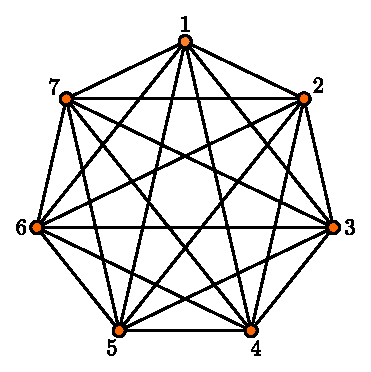
\includegraphics[width=0.4\textwidth]{Figuras/grafo-k7.pdf}
\caption{Uma representação de $K_7$.}
\label{Rotulo}
\end{figure}
\end{center}
%%%

{\bf Colorações de $K_n$.}
Uma coloração de $K_n=(V_n,E_n)$ em duas cores 
é uma função $c:E_n\to \{0,1\}$.
Seja $e\in E_n$ uma aresta de $K_n$. 
Dizemos que $e$ está colorida de azul se $c(e)=0$, 
caso $c(e)=1$ vamos dizer que $e$ está colorida de vermelho.

Fixada uma coloração $c$ de $K_n$ e um número natural $k<n$, 
dizemos que $K_n$ possui um subgrafo monocromático
{\bf azul} $K_k$, se existem $k$ vértices 
$\{v_1,\ldots,v_k\}\subset \{1,\ldots,n\}$
tais que $c(\{v_i,v_j\})=0$ para todo $i,j=1,\ldots,k$
com $i\neq k$. Analogamente definimos $K_k$ 
monocromático {\bf vermelho}.


O número de Ramsey $R(k,l)$ é o menor inteiro
$n$ tal que qualquer coloração $c:E_n\to\{0,1\}$
de $K_n$ possui pelo menos um subgrafo $K_k$ monocromático azul 
ou um subgrafo $K_l$ monocromático vermelho.

Em 1929 Ramsey mostrou que $R(k,l)$ é finito para 
quaisquer inteiros $k$ e $l$. 
Nosso objetivo neste exercício será 
exibir cotas inferior e superior para 
os números de Ramsey da diagonal, isto é, 
$R(k,k)$.

	\begin{itemize}
		\item[a)] 
		Construa um espaço de probabilidade 
		$(\Omega,\F,\P)$ e defina o que é uma coloração aleatória 
		de $K_n$. 
		
		\item[b)] Mostre que existe uma coloração aleatória de $K_n$,
		onde cada aresta de $E_n$ é colorida aleatoriamente
		de azul ou vermelho com igual probabilidade.
		
		\item[b)] Para qualquer conjunto $R$ possuindo $k$ ($k\leq n$)
		vértices em $K_n$, 
		seja $A_R$ o evento o subgrafo de $K_n$ induzido 
		por $R$ é monocromático, isto é, todas as arestas
		de vértices em $R$ estão pintadas com a mesma cor. 
		Mostre que
			\[ 
				\P(A_R) = \frac{1}{2^{\binom{n}{k}-1  }}
			\]
		
		\item[c)] Mostre que a probabilidade de pelo menos um 
		evento do tipo $A_R$ ocorrer é no máximo 
			\[
				\binom{n}{k}\frac{1}{2^{\binom{n}{k}-1  }}.
			\]
			
		\item[d)] Mostre que se $n$ e $k$ satisfazem
			\[
				\binom{n}{k}\frac{1}{2^{\binom{n}{k}-1  }} < 1
			\]
		então $R(k,k)> n$.
		
		\item[e)] Mostre que se $n=\lfloor 2^{k/2} \rfloor$ então
			\[
				\binom{n}{k}\frac{1}{2^{\binom{n}{k}-1  }} < 1.
			\]
		Conclua que $R(k,k)> \lfloor 2^{k/2} \rfloor $ para todo 
		$k\geq 3$.		
		
		\item[f)] Leia. É fácil mostrar que $R(3,3)=6$. 
		O valor de $R(4,4)=18$ foi determinado apenas em 1979 
		por 	Evans, Pulham e Sheehan. 
		O valor de $R(k,k)$ para $k\geq 5$ não é conhecido ainda.
		Em uma entrevista o famoso matemático Paul Erdös 
		explica usando a seguinte anedota,
		o grau de dificuldade de se calcular exatamente
		tais números com a tecnologia matemática disponível atualmente: \\
		`` Suponha que uma civilização alienígena muito 
		mais desenvolvida e poderosa que a nossa, 
		pouse sobre a Terra e exija que façamos o cálculo do valor
		exato de $R(5,5)$ ou caso contrário, eles destruirão nosso planeta. 
		Neste caso, 
		na minha opinião, a melhor estratégia é pegar todos os matemáticos e todos
		os computadores do mundo e tentar encontrar este valor.
		Mas, se os alienígenas exigirem o valor exato de $R(6,6)$,
		eu acredito que 	a melhor estratégia seja destruí-los.''
		 
	\end{itemize}























\end{enumerate}









%%%%%%%%%%%%%%%%%% Referências e Índice Remissivo
\backmatter
%
%\chapter{Referências}
%\include{./referencias/referencias}

%\printindex
%\chapter{Índice de Símbolos}


\end{document}
